% -----------------------------------------------------------------------------
% Master thesis in the study program computational mechanics
%
% B.Sc. Rezha Adrian Tanuharja - 03751261
% M.Sc. Felix Schneider (supervisor)
%
% main.tex
% Last edited 03 November 2023
% -----------------------------------------------------------------------------

\documentclass[%
  12pt,
  a4paper,
  twoside,
  headinclude,
  headsepline,
  plainheadsepline,
  BCOR=12mm,
  DIV=18,
  parskip=half,
  openany,
  bibliography=totoc,
  toc=listof,
  numbers=noenddot,
  captions=tableheading,
  fleqn
]{bmvorlagen/bmthesis}


% ----- Additional packages and custom settings -------------------------------

% -----------------------------------------------------------------------------
% Master thesis in the study program computational mechanics
%
% B.Sc. Rezha Adrian Tanuharja - 03751261
% M.Sc. Felix Schneider (supervisor)
%
% settings.tex
% Last edited 03 November 2023
% -----------------------------------------------------------------------------


% ----- Additional packages ---------------------------------------------------

\usepackage[utf8]{inputenc}
\usepackage[T1]{fontenc}
\usepackage[ruled]{algorithm2e}


% ----- Additional TikZ libraries for sketches and flowcharts -----------------

\usetikzlibrary{patterns,shapes,arrows,calc}


% ----- Custom column types for tables ----------------------------------------

\newcolumntype{L}[1]{
  >{\raggedright\let\newline\\\arraybackslash\hspace{0pt}}m{#1}
}
\newcolumntype{C}[1]{
  >{\centering\let\newline\\\arraybackslash\hspace{0pt}}m{#1}
}
\newcolumntype{R}[1]{
  >{\raggedleft\let\newline\\\arraybackslash\hspace{0pt}}m{#1}
}


% ----- Other settings --------------------------------------------------------

\setlength{\marginparwidth}{2cm}


% ----- Settings for flowcharts' spacing --------------------------------------

\def\chartvgap{1.5cm}
\def\charthgap{7.0cm}
\def\charttwid{6.0cm}
% -----------------------------------------------------------------------------
% Master thesis in the study program computational mechanics
%
% B.Sc. Rezha Adrian Tanuharja - 03751261
% M.Sc. Felix Schneider (supervisor)
%
% includes/algorithmFunctions.tex
% Last edited 03 November 2023
% -----------------------------------------------------------------------------


% ----- Functions for eigenproblem and eigenmodes -----------------------------

\SetKwFunction{genEigSol}{generalizedEigensolver}
\SetKwFunction{modeSelector}{modeSelector}


% ----- Functions for dynamic substructuring ----------------------------------

\SetKwFunction{craigBampton}{craigBampton}
\SetKwFunction{enhancedCB}{enhancedCraigBampton}


% ----- Functions for Message Passing Interface (MPI) -------------------------

\SetKwFunction{mpiInit}{MPI\_init}
\SetKwFunction{mpiFinalize}{MPI\_finalize}
\SetKwFunction{mpiGather}{MPI\_gather}
\SetKwFunction{mpiBroadcast}{MPI\_broadcast}


% ----- Functions for surrogate model and regression --------------------------

\SetKwFunction{lsRegression}{leastSquareRegression}
\SetKwFunction{detCoeff}{detCoeff}
\SetKwFunction{err}{err}

\SetKwFunction{trainRPCE}{trainRPCE}
\SetKwFunction{computeRPCE}{computeRPCE}
\SetKwFunction{looRPCE}{looRPCE}

\SetKwFunction{basisSelector}{basisSelector}


% ----- General functions -----------------------------------------------------

\SetKwFunction{sample}{sample}
\SetKwFunction{zeros}{zeros}

\SetKwFunction{sum}{sum}
\SetKwFunction{numel}{numel}
\SetKwFunction{len}{len}


% ----- Meta information about the thesis -------------------------------------

\newcommand{\bmtitle}{%
  Non-Intrusive Surrogate Modelling for Stochastic Linear Structural Systems Based on Collocation Using Substructuring Methods
}
\newcommand{\bmauthor}{B.Sc. Rezha Adrian Tanuharja}

\newcommand{\bmkeywords}{%
  Craig-Bampton Method,
  Linear Structural Dynamics,
  Non-Intrusive Rational Polynomial Chaos Expansion,
  Sparse Surrogate Model,
  Uncertainty Quantification
}

\newcommand{\bmstartpage}{5}


% ----- Contents --------------------------------------------------------------

\raggedbottom

\begin{document}

\frontmatter

\pagenumbering{Roman}

\begin{titlepage}
	%\layout
	
	\begin{center}
		{
			\fontsize{18}{18}\selectfont 
			
			\includegraphics*[width=3cm, keepaspectratio=true]{bmvorlagen/logos/tumlogo} \hfill \includegraphics*[width=2.5cm, keepaspectratio=true]{bmvorlagen/logos/bmlogo}
			\vspace{0.5cm}
			\hrule
			
			\vspace{1cm}
			Chair of Structural Mechanics\\
			Technical University of Munich\\
			
			\vspace{1.4cm}
			
			\vspace{2cm}
			
			
			\vspace{3mm}
			
			
			
			\bmtitle \\[5ex]
			
			
			\bmauthor \\[7ex]
			
			
			Master thesis in the study program computational mechanics\\
			Focus area Structural Dynamics\\
			
			\vspace{1.8cm}
			
			{\fontsize{12pt}{12} \selectfont%
				\begin{tabular}{rll}
					Editor&:& Univ.-Prof. Dr.-Ing. Gerhard Müller\\
					& & Dr.-Ing. Francesca Taddei\\[0.5ex]
					Supervisor&:& M.Sc. Felix Schneider\\[0.5ex]
					Handed in&:& \today
				\end{tabular}
			}
			
			
		}
	\end{center}
	
\end{titlepage}
\cleardoubleemptypage

% -----------------------------------------------------------------------------
% Master thesis in the study program computational mechanics
%
% B.Sc. Rezha Adrian Tanuharja - 03751261
% M.Sc. Felix Schneider (supervisor)
%
% decorators/abstract.tex
% Last edited 03 November 2023
% -----------------------------------------------------------------------------

\addchap{Abstract}
\label{cha:abtract} 

This thesis introduces a novel framework for uncertainty quantification in linear structural dynamics.
The framework uses the well-established Craig-Bampton (CB) method to generate the training data for a recently developed non-intrusive rational polynomial chaos expansion (NI-RPCE) model.
A modification to the CB method takes place, reducing its computational cost in a Monte Carlo simulation (MCS) for models with varying input parameters.
In addition, the author develops a new approach to building a sparse NI-RPCE model, thus reducing the required size of the training data.
As a result, the proposed framework provides an efficient and scalable means to tackle large and complex structures.
The scope covers time-invariant structures with parametric uncertainties.
The thesis includes a case study to compare the new framework with a classic uncertainty quantification approach: the direct MCS.


Keywords: 
\begin{itemize}
 \item Craig-Bampton Method
 \item Linear Structural Dynamics
 \item Non-Intrusive Rational Polynomial Chaos Expansion
 \item Sparse Surrogate Model
 \item Uncertainty Quantification
\end{itemize}
% -----------------------------------------------------------------------------
% Master thesis in the study program computational mechanics
%
% B.Sc. Rezha Adrian Tanuharja - 03751261
% M.Sc. Felix Schneider (supervisor)
%
% decorators/declaration.tex
% Last edited 03 November 2023
% -----------------------------------------------------------------------------

\addchap{Declaration}
\markboth{Declaration}{Declaration}
\label{cha:erkl}

\subsubsection{Acknowledgements}
Completing this Master's thesis would not be possible without the valuable contributions and support of numerous individuals.
The author's gratitude extends to the following:

\textbf{Thesis Supervisor, M.Sc. Felix Schneider}: The author is grateful for the expertise, guidance, support, and constructive feedback that have been instrumental in shaping this thesis.

\textbf{Computational Mechanics Students at TUM}: The author appreciates the camaraderie and intellectual discussion, which enriched the academic journey.

\textbf{Family and Friends}: A special recognition for their unwavering support and for making everything worthwhile.

\subsubsection{Declaration}
I hereby certify that I have completed this work independently and without outside help.
The literature and other resources used are listed in full.
\vfill
M\"{u}nchen, \today \\
\vspace{3cm} \\
Rezha Adrian Tanuharja
\vfill
\cleardoubleemptypage

\begin{spacing}{1.0}
  \tableofcontents
  \listoffigures
  \listoftables
\end{spacing}

% -----------------------------------------------------------------------------
% Master thesis in the study program computational mechanics
%
% B.Sc. Rezha Adrian Tanuharja - 03751261
% M.Sc. Felix Schneider (supervisor)
%
% decorators/symbols.tex
% Last edited 03 November 2023
% -----------------------------------------------------------------------------

\addchap{Symbols}
\markboth{Symbolverzeichnis}{Symbolverzeichnis}
\label{cha:symbolverzeichnis}

The addition $\hat{\medspace}$ represents an approximation.\\
The addition $\bar{\medspace}$ represents a value in a modal space.

\section*{Greek Letters}
\begin{longtable}[l]{lcp{8cm}l}
$\lambda$ & & Eigenvalue \\
$\omega$ & \einheit{\frac{rad}{s}} & Angular Frequency \\
$\Psi$ & & Multivariate Basis Function \\
$\xi$ & & Zero-Mean Random Variable \\
\\
$\mathbf{\Phi}$ & & Eigenmode Matrix \\
$\mathbf{\Xi}$ & & Vector of zero-mean random variables\\
\end{longtable}

\section*{Latin Letters}
\begin{longtable}[l]{lcp{8cm}l}
%\hspace*{2.5cm}\= \hspace*{1cm} \=  Schallschnelle senkrecht zu einer Oberfläche \= \kill
$\mathbf{C}$ & \einheit{\frac{N}{m\cdot s}} & Damping Matrix\\
$\mathbf{D}$ & \einheit{\frac{N}{m}} & Dynamic Stiffness Matrix\\
$\mathbf{F}$ & \einheit{N} & Force Vector\\
$\mathbf{G}$ & \einheit{N} & Coupling Force Vector\\
$\mathbf{H}$ & \einheit{\frac{m}{N\cdot s^{2}}} & Frequency Response Function Matrix\\
$\mathbf{I}$ & & Identity Matrix\\
$\mathbf{K}$ & \einheit{\frac{N}{m}} & Stiffness Matrix\\
$\mathbf{M}$ & \einheit{kg} & Mass Matrix\\
$\mathbf{U}$ & \einheit{m} & Generalized Displacement Vector\\
$\mathbf{X}$ & & Modal Displacement Vector\\
\end{longtable}


\cleardoubleplainpage

\mainmatter

% -----------------------------------------------------------------------------
% Master thesis in the study program computational mechanics
%
% B.Sc. Rezha Adrian Tanuharja - 03751261
% M.Sc. Felix Schneider (supervisor)
%
% chapters/introduction.tex
% Last edited 03 November 2023
% -----------------------------------------------------------------------------

\chapter{Introduction}
\label{ch: introduction}

In structural dynamics, numerical simulations play a vital role in predicting and understanding the dynamic response of engineering systems.
However, the simulation parameters are rarely, if ever, precisely known.
The development of methods to account for this uncertainty is still an active field of research.
A particular challenge is to devise strategies to cope with the computational cost associated with large and complex structures.
This thesis formulates a novel framework to tackle this challenge.

% -----------------------------------------------------------------------------
% Master thesis in the study program computational mechanics
%
% B.Sc. Rezha Adrian Tanuharja - 03751261
% M.Sc. Felix Schneider (supervisor)
%
% chapters/introduction/background.tex
% Last edited 03 November 2023
% -----------------------------------------------------------------------------

\section{Background}
\label{sec: background}

Structures can have numerous elements and interacting parts.
Each element adds to the system's degrees of freedom (DOFs).
As structures become more complex, their dynamic analysis becomes increasingly expensive because one must simultaneously compute more DOFs.
Component mode synthesis (CMS) addresses this challenge by dividing the structure into smaller components and models the dynamic behavior and interactions of these components \cite{hurty1960vibrations}\cite{hurty1965dynamic}.
This component-wise analysis is faster and more cost-effective than evaluating the complete structure simultaneously.

As the benefit of CMS became apparent, further development followed, which led to the classic Craig-Bampton (CB) method in \cite{craig1968coupling}.
The method distinguishes the components' internal dynamic responses from intercomponent interactions via a modal decomposition.
By performing mathematical reduction on the internal dynamic model, the CB method reduces the number of DOFs and, therefore, the computational cost.
However, the reduction introduces a discrepancy between the assembly of these components and the original structure.
Consequently, there have been several efforts to improve the accuracy of the CB method, such as the flexibility-based CMS (F-CMS) \cite{park2004partitioned} and the enhanced CB (ECB) method \cite{kim2015enhanced}\cite{boo2018towards}.
Regardless, the CB method is still popular because of its simplicity.

Like most available approaches, the CB method assumes that all structural parameters are precisely known.
In reality, this is seldom the case.
Therefore, uncertainty quantification due to variability in the structural parameters is necessary.
Several publications have combined CMS and the CB method with uncertainty quantification methods, such as the perturbation method \cite{hinke2009component}\cite{sarsri2016dynamic}, the stochastic reduced basis projection \cite{dohnal2009joint}, and neural networks \cite{chatterjee2021multilevel}.

In a separate context, surrogate modeling has emerged as a popular method for uncertainty quantification in structural dynamics.
An example of a surrogate model is the polynomial chaos expansion (PCE), which approximates model outputs using linear combinations of multivariate polynomials.
There are various means to obtain the polynomials' coefficients, including the stochastic Galerkin method \cite{Ghanem1991}, numerical quadrature \cite{xiu2007efficient}, interpolation \cite{babuvska2007stochastic}, and various regression techniques \cite{berveiller2006stochastic}\cite{blatman2010adaptive}\cite{blatman2011adaptive}.

Despite its popularity, PCE performs poorly in approximating frequency response functions around structures' eigenfrequencies \cite{jacquelin2015polynomial}.
Authors of \cite{jacquelin2017polynomial} proposed to approximate model outputs using ratios of PCEs (RPCE) instead, using the stochastic Galerkin method to compute the PCEs' coefficients.
The authors of the paper show that RPCE requires a lower number of basis functions to approximate highly nonlinear models compared to PCE.

Recently, the authors of \cite{schneider2020polynomial} developed the non-intrusive RPCE (NI-RPCE), using regression to compute the coefficients.
This model saw further development in \cite{schneider2023sparse}, in which sparse Bayesian learning helps to avoid overfitting.
An attractive feature of NI-RPCE is that it approximates each output independently.
Therefore, the CB method and NI-RPCE combination may be promising for uncertainty propagation as the surrogate model can approximate each component's dynamic response separately.
% -----------------------------------------------------------------------------
% Master thesis in the study program computational mechanics
%
% B.Sc. Rezha Adrian Tanuharja - 03751261
% M.Sc. Felix Schneider (supervisor)
%
% chapters/introduction/objectives.tex
% Last edited 03 November 2023
% -----------------------------------------------------------------------------

\section{Research Objectives}
\label{sec: objectives}

The primary objective of this research is to develop and demonstrate a novel framework for uncertainty quantification of large and complex structures by combining the well-established CB method with the recently developed NI-RPCE.
Specifically, this study aims to achieve the following objectives:

\begin{itemize}
    \item Modify the CB method, optimizing it to analyze structures' dynamic responses with varying simulation parameters.
    \item Modify a sparse regression technique to work with the rational form of NI-RPCE and mitigate overfitting.
    \item Integrate the modified CB method, NI-RPCE, and the modified sparse regression technique into a framework for uncertainty quantification for large and complex structures.
    \item Demonstrates the effectiveness of the developed framework using a case study.
\end{itemize}
% -----------------------------------------------------------------------------
% Master thesis in the study program computational mechanics
%
% B.Sc. Rezha Adrian Tanuharja - 03751261
% M.Sc. Felix Schneider (supervisor)
%
% chapters/introduction/significance.tex
% Last edited 03 November 2023
% -----------------------------------------------------------------------------

\section{Significance of The Study}
\label{sec: significance}

This study develops a novel framework for uncertainty quantification in structural dynamics.
By combining well-established methods with a recently developed approach, the framework provides an efficient and scalable means to evaluate large and complex structures.
Beyond its immediate application, this research advances existing knowledge and facilitates future development in the field.
% -----------------------------------------------------------------------------
% Master thesis in the study program computational mechanics
%
% B.Sc. Rezha Adrian Tanuharja - 03751261
% M.Sc. Felix Schneider (supervisor)
%
% chapters/introduction/scope.tex
% Last edited 03 November 2023
% -----------------------------------------------------------------------------

\section{Scope and Limitations}
\label{sec: scope}

This study aims to develop a new framework for uncertainty quantification of linear time-invariant structures.
The proposed framework propagates uncertainties in structural parameters to the structure's frequency response functions at discrete frequencies.
This study includes a comparative analysis between the developed framework and the direct Monte Carlo (MC) method.

While the framework is suitable for parallel computing, the focus is not on developing its high-performance implementations.
The study also uses simple numerical examples, such that the direct MC method remains feasible with the time constraints and available computational resources.
% -----------------------------------------------------------------------------
% Master thesis in the study program computational mechanics
%
% B.Sc. Rezha Adrian Tanuharja - 03751261
% M.Sc. Felix Schneider (supervisor)
%
% chapters/introduction/structure.tex
% Last edited 03 November 2023
% -----------------------------------------------------------------------------

\section{Structure of The Thesis}
\label{sec: structure}

Chapter \ref{ch: literature review} contains relevant literature studies about dynamic substructuring methods, non-intrusive surrogate models, and sparse regression.
Chapter \ref{ch: development} documents the development of the new framework.
Chapter \ref{ch: methodology} presents the methodology and performance measures used in this study, and the case study to demonstrate the effectiveness of the developed framework.
Chapter \ref{ch: discussion} discusses observations and findings made during the research.
The thesis ends in chapter \ref{ch: conclusion} with the summary and conclusion.
% -----------------------------------------------------------------------------
% Master thesis in the study program computational mechanics
%
% B.Sc. Rezha Adrian Tanuharja - 03751261
% M.Sc. Felix Schneider (supervisor)
%
% chapters/literature.tex
% Last edited 03 November 2023
% -----------------------------------------------------------------------------

\chapter{Literature Review}
\label{ch: literature review}

% -----------------------------------------------------------------------------
% Master thesis in the study program computational mechanics
%
% B.Sc. Rezha Adrian Tanuharja - 03751261
% M.Sc. Felix Schneider (supervisor)
%
% chapters/discussion/substructuring.tex
% Last edited 03 November 2023
% -----------------------------------------------------------------------------

\section{Dynamic Substructuring}
\label{sec: performance of cms}

This section reports the findings from the first half of the proposed framework: dynamic substructuring for models with parametric uncertainties. 
These findings come from observing the plate's vertical acceleration at nodes A and B when subjected to a unit vertical force at node A.
Details about the nodes are available in chapter \ref{ch: methodology}.

% -----------------------------------------------------------------------------
% Master thesis in the study program computational mechanics
%
% B.Sc. Rezha Adrian Tanuharja - 03751261
% M.Sc. Felix Schneider (supervisor)
%
% chapters/discussion/substructuring/point_A.tex
% Last edited 03 November 2023
% -----------------------------------------------------------------------------

\subsection{Vertical Acceleration at Node A}
\label{ssec: cms point A}

Figure \ref{FRF_MC_A_A_linear} shows the FRFs from direct MCS of the complete plate model.
These FRFs relate the vertical acceleration magnitude at point A to a unit force at the same point at discrete frequencies in the range $\left[9.0, 17.5\right]$ rad/s with increments of $0.5$ rad/s.
The outliers are intentionally missing to enable a clear view of the FRFs' statistics: their medians, interquartile ranges, and whiskers.
\begin{figure}[H]
    \centering
    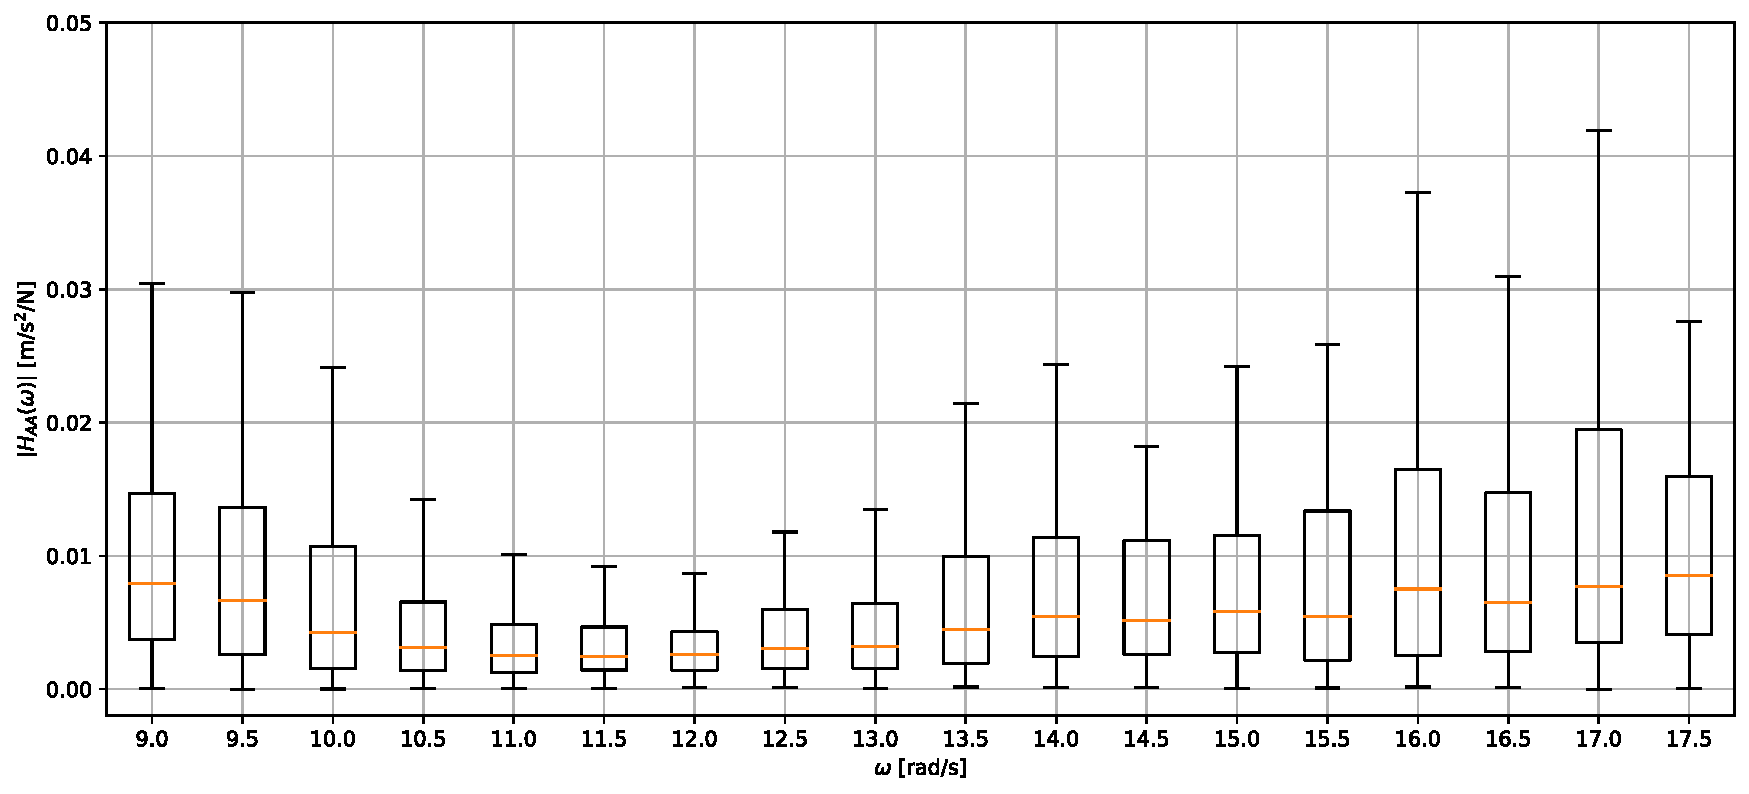
\includegraphics[width=1.0\textwidth]{
        plots/substructuring/plot_1_linear.pdf
    }
    \caption{%
        $\left|H_{AA}\right|$ from Direct MCS of The Complete Plate Model
    }
    \label{FRF_MC_A_A_linear}
\end{figure}
Figure \ref{FRF_MC_A_A_log} shows the same FRFs as figure \ref{FRF_MC_A_A_linear} with outliers.
The logarithmic scale provides a clear view of the outliers and the low whiskers of the plot.
The figure shows that the outlier values can be larger by approximately two orders of magnitudes compared to the medians.
\begin{figure}[H]
    \centering
    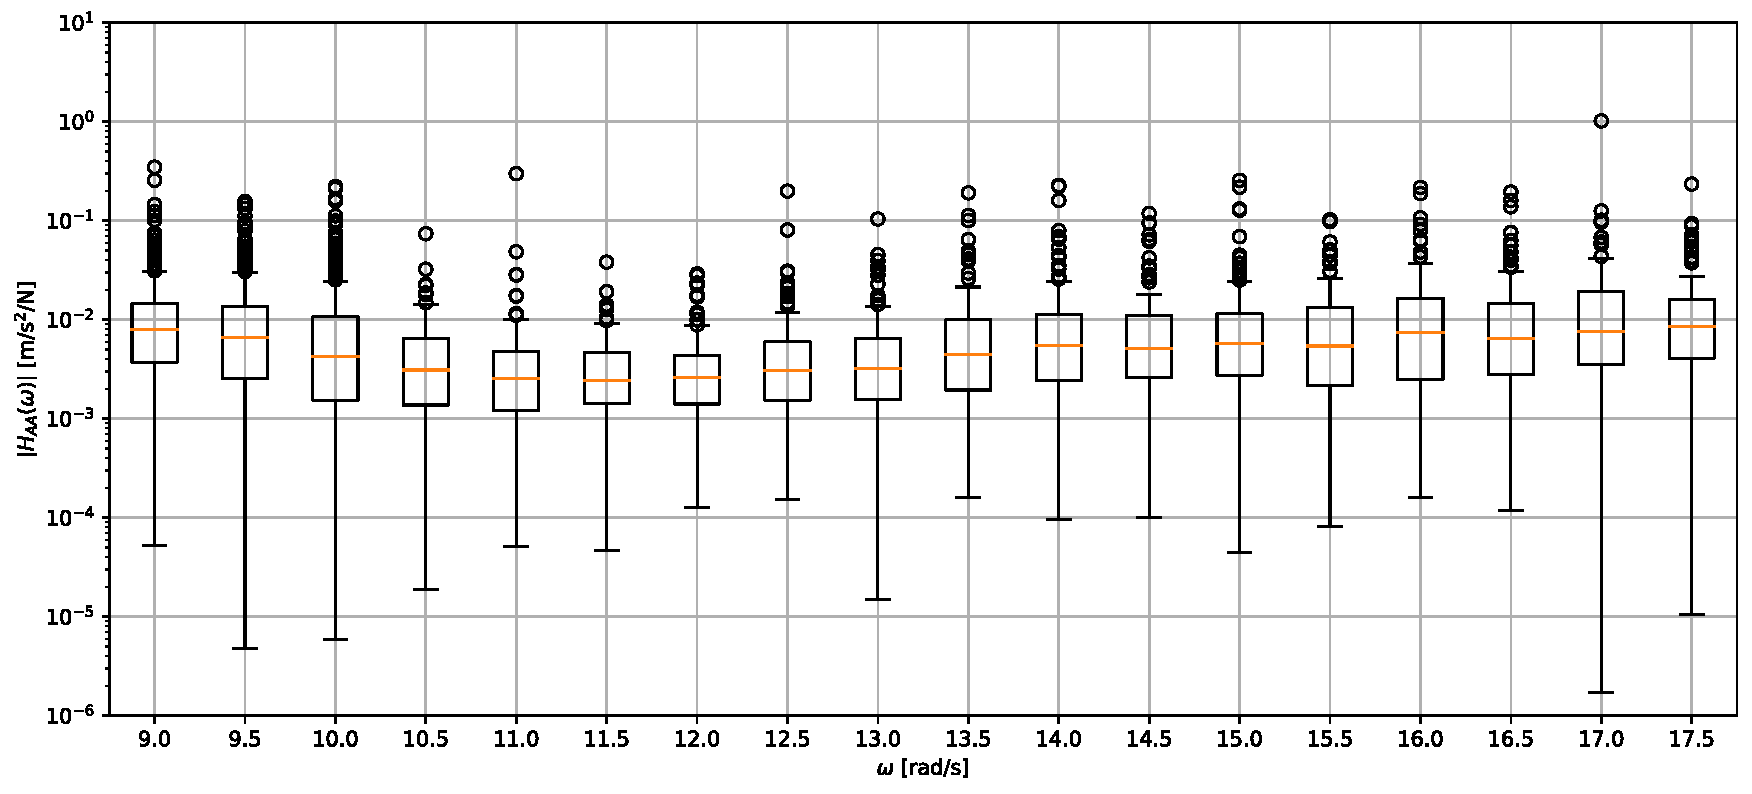
\includegraphics[width=1.0\textwidth]{
        plots/substructuring/plot_1_log.pdf
    }
    \caption{%
        $\left|H_{AA}\right|$ from Direct MCS of The Complete Plate Model with Outliers
    }
    \label{FRF_MC_A_A_log}
\end{figure}
First, the author analyzes the performance of the CUCB method.
Figure \ref{e_emp CUCB_A_A} shows the median relative empirical errors for the method in each frequency in the above range using three different numbers of internal modes.
The medians come from the bootstrapping method with a $1000$ number of resamplings.
\begin{figure}[H]
    \centering
    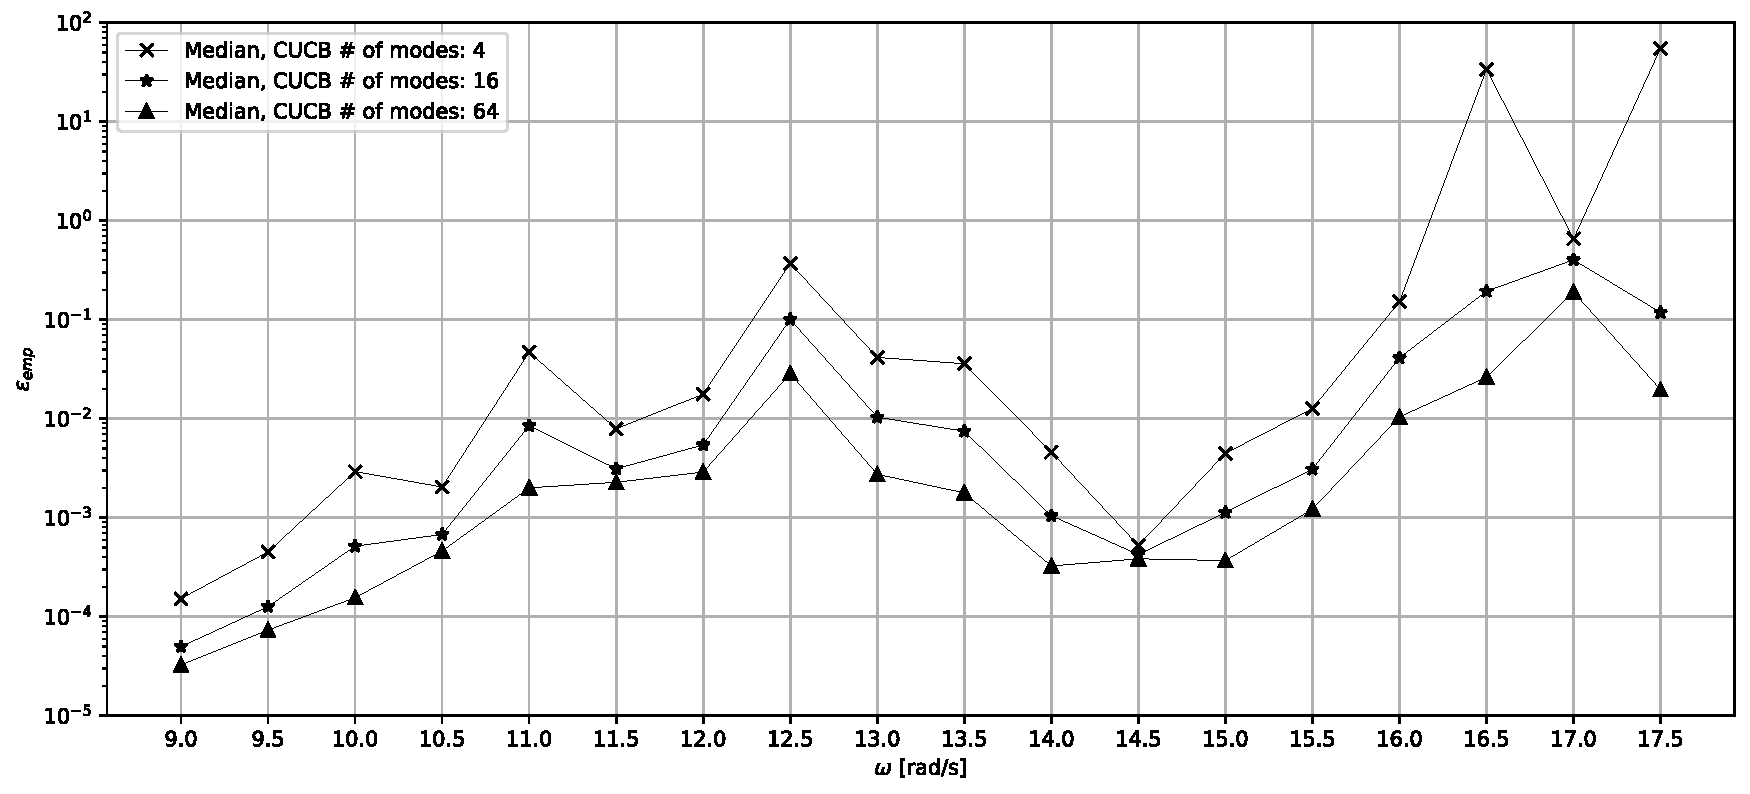
\includegraphics[width=1.0\textwidth]{
        plots/substructuring/plot_2.pdf
    }
    \caption{%
        Relative Empirical Errors of $H_{AA}$ for The CUCB Method
    }
    \label{e_emp CUCB_A_A}
\end{figure}
In deterministic dynamic substructuring, errors decrease as the number of internal modes increases.
When all internal modes are present in the model, the assembled components are equivalent to the complete structure in a mathematical sense.
Figure \ref{e_emp CUCB_A_A} exhibits the same trend for dynamic structuring using the CUCB method: as the number of internal modes increases, the relative empirical errors decrease.
However, the relative empirical errors exceeds $10^{-1}$ at $\omega=17.0$ rad/s even when using $64$ internal modes.
Therefore, the mean square errors are in the same order of magnitude as the FRFs' variance at this frequency.

Subsequently, the author analyzes the performance of the HUCB method.
Figure \ref{e_emp HUCB_A_A} shows the medians and $95\%$ confidence intervals of the relative empirical errors for the crude and hybrid UCB methods.
Figure \ref{e_emp HUCB_A_A} shows that the relative empirical errors from the HUCB method do not exceed $10^{-2}$ in this example and in most frequencies in the range lie below $10^{-3}$.
The computational cost of the HUCB method is higher than that of the CUCB method because of the evaluation of the boundary modes for each input parameter's realization.
However, it leads to lower overall relative empirical errors and, in some frequencies, reduces the errors by up to two orders of magnitudes.
\begin{figure}[H]
    \centering
    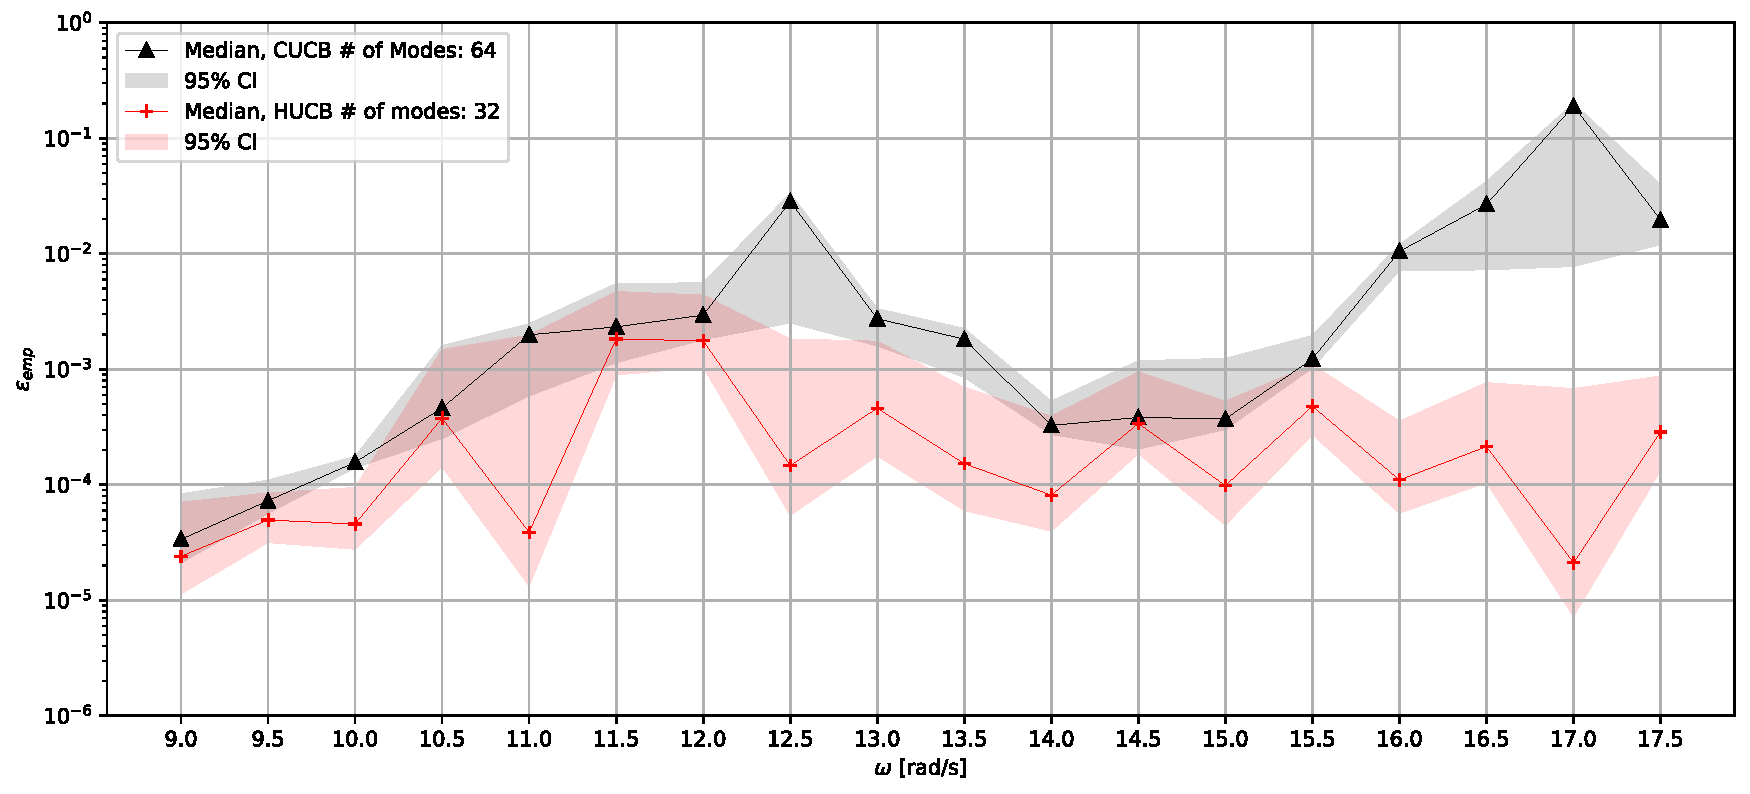
\includegraphics[width=1.0\textwidth]{
        plots/substructuring/plot_3.pdf
    }
    \caption{%
        Relative Empirical Errors of $H_{AA}$ for The CUCB and HUCB Methods
    }
    \label{e_emp HUCB_A_A}
\end{figure}

To dive deeper into the difference between the crude and hybrid UCB methods, the author evaluates the relative mean and variance errors.
Figure \ref{e_mean CUCB_A_A} shows the median relative mean errors of the FRFs' magnitudes for the CUCB method using three different numbers of internal modes.
\begin{figure}[H]
    \centering
    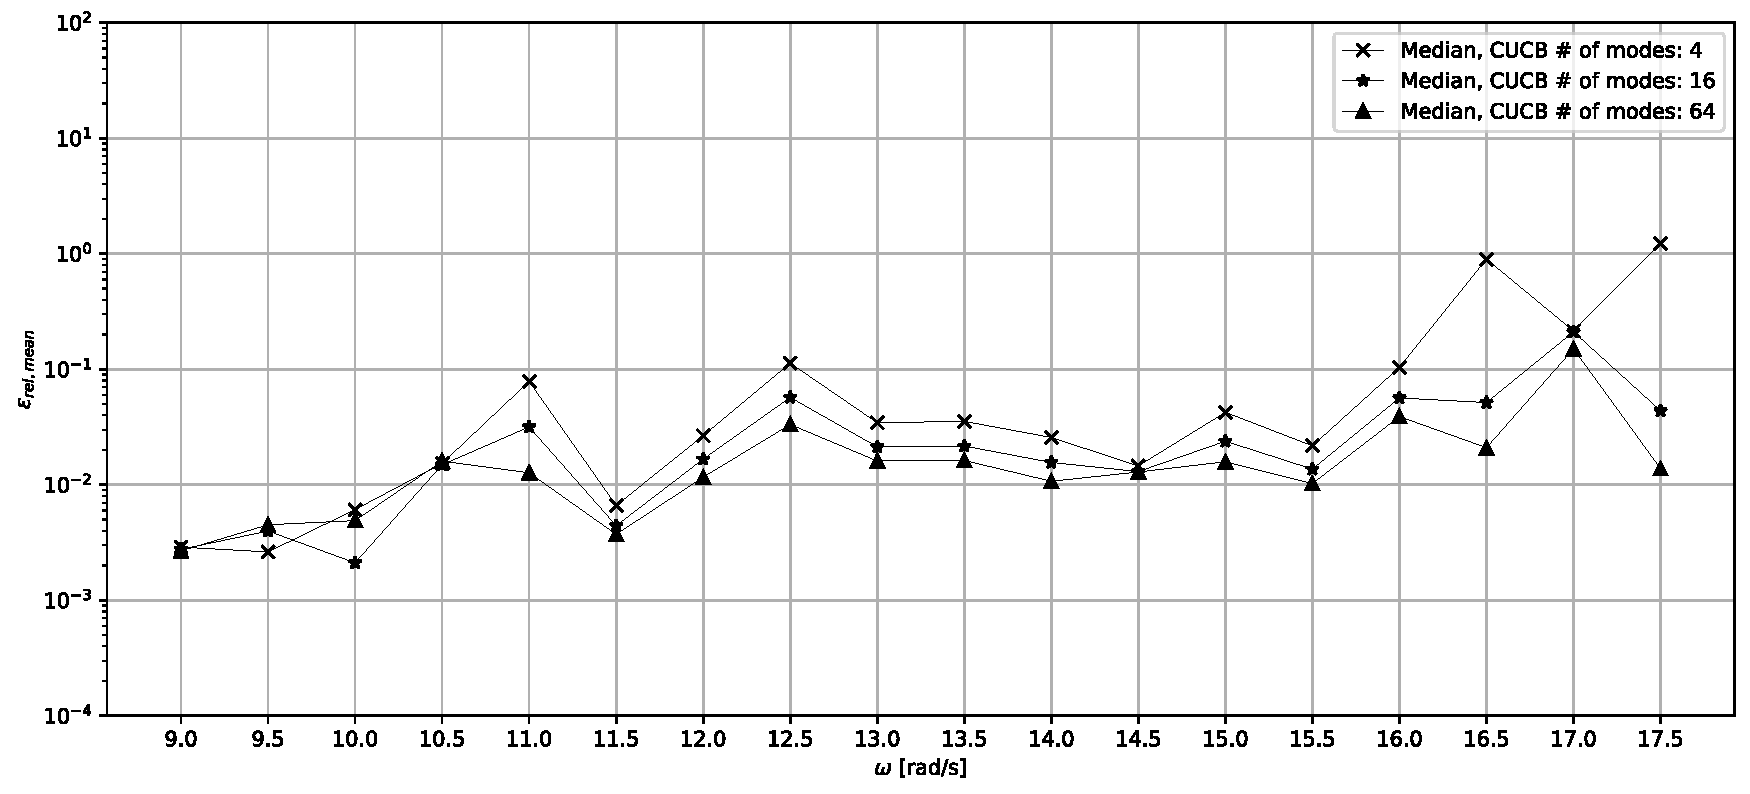
\includegraphics[width=1.0\textwidth]{
        plots/substructuring/plot_4.pdf
    }
    \caption{%
        Relative Mean Errors of $\left|H_{AA}\right|$ for The CUCB Method
    }
    \label{e_mean CUCB_A_A}
\end{figure}
Figure \ref{e_var CUCB_A_A} shows the median relative variance errors of the FRFs for the CUCB method using three different numbers of internal modes.
\begin{figure}[H]
    \centering
    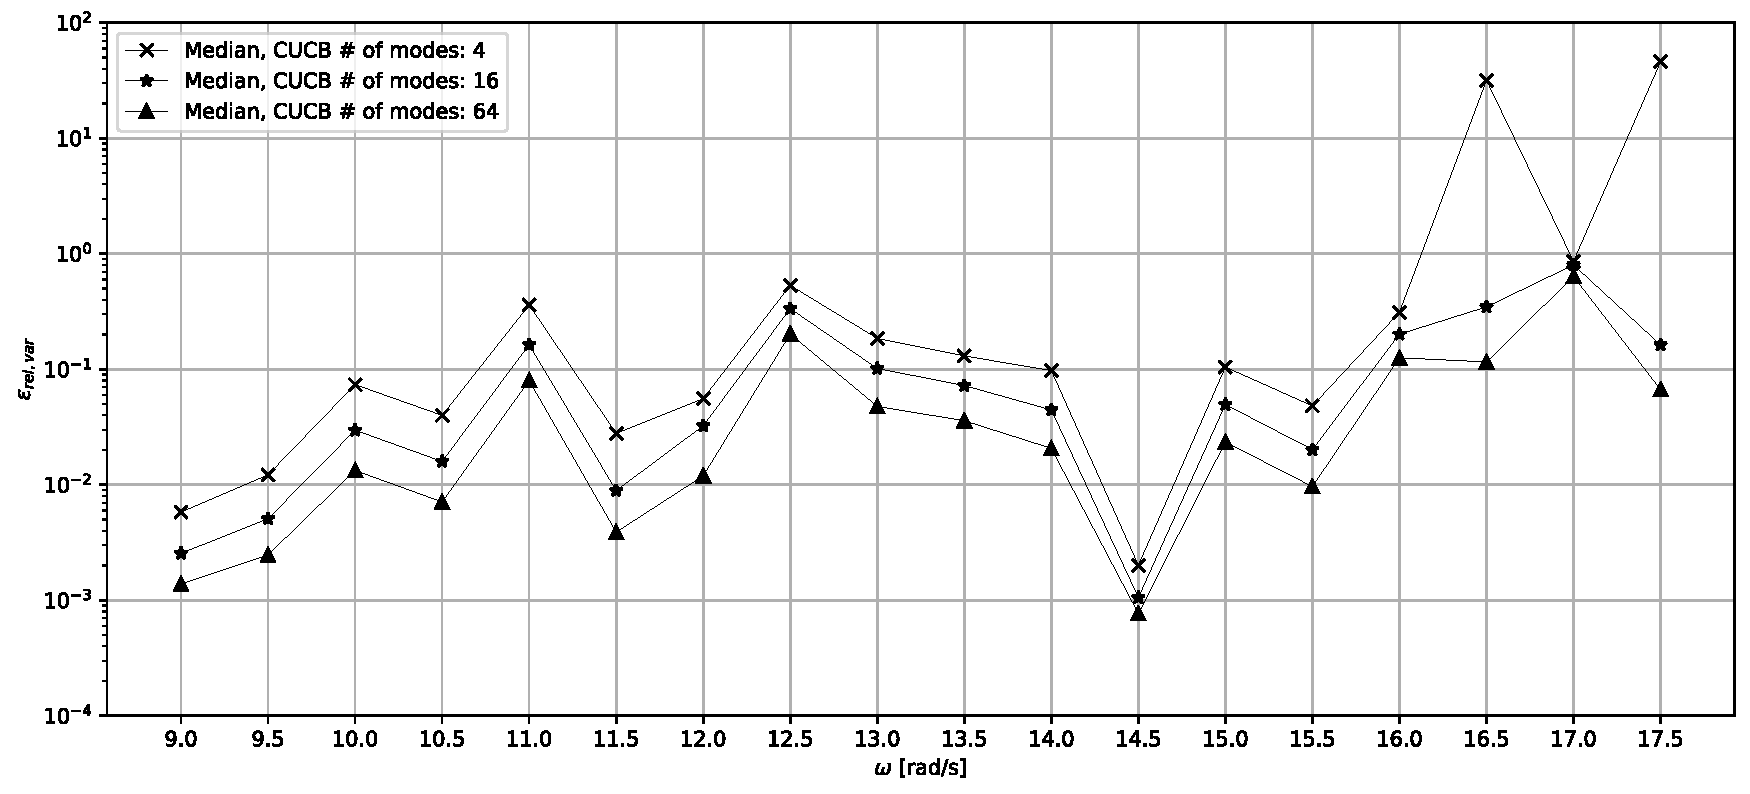
\includegraphics[width=1.0\textwidth]{
        plots/substructuring/plot_5.pdf
    }
    \caption{%
        Relative Variance Errors of $H_{AA}$ for The CUCB Method
    }
    \label{e_var CUCB_A_A}
\end{figure}
The two figures above exhibit similar trends with figure \ref{e_emp CUCB_A_A}: the relative mean errors decrease as the number of internal modes increases, with an exception at $\omega=9.5$ rad/s for the relative mean errors.
Overall, the relative mean errors and relative variance errors primarily lie between $10^{-3}$ and $10^{0}$.

Subsequently, the author compares the relative mean errors and relative variance errors for the CUCB method and the HUCB method.
Figure \ref{e_mean HUCB_A_A} shows the medians and $95\%$ confidence intervals of the relative mean errors of the FRFs' magnitudes in each frequency in the above range for the crude and hybrid UCB methods.
\begin{figure}[H]
    \centering
    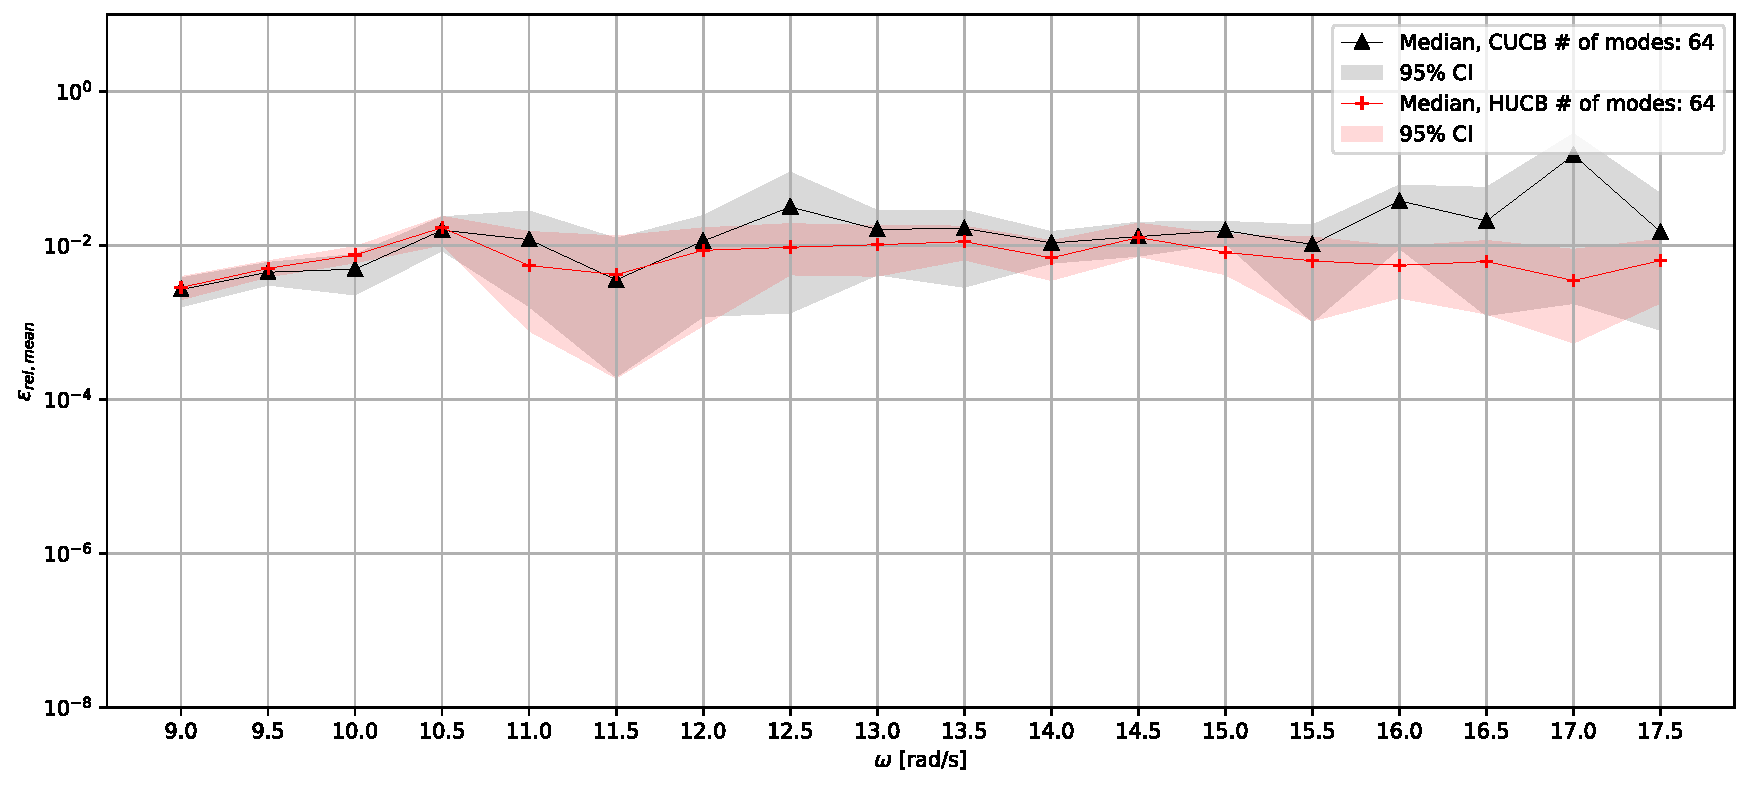
\includegraphics[width=1.0\textwidth]{
        plots/substructuring/plot_6.pdf
    }
    \caption{%
        Relative Mean Errors of $\left|H_{AA}\right|$ for The CUCB and HUCB Methods
    }
    \label{e_mean HUCB_A_A}
\end{figure}
Figure \ref{e_var HUCB_A_A} shows the median and $95\%$ confidence interval of the relative variance error for the FRFs' magnitudes in each frequency in the above range using the crude and hybrid UCB methods.
\begin{figure}[H]
    \centering
    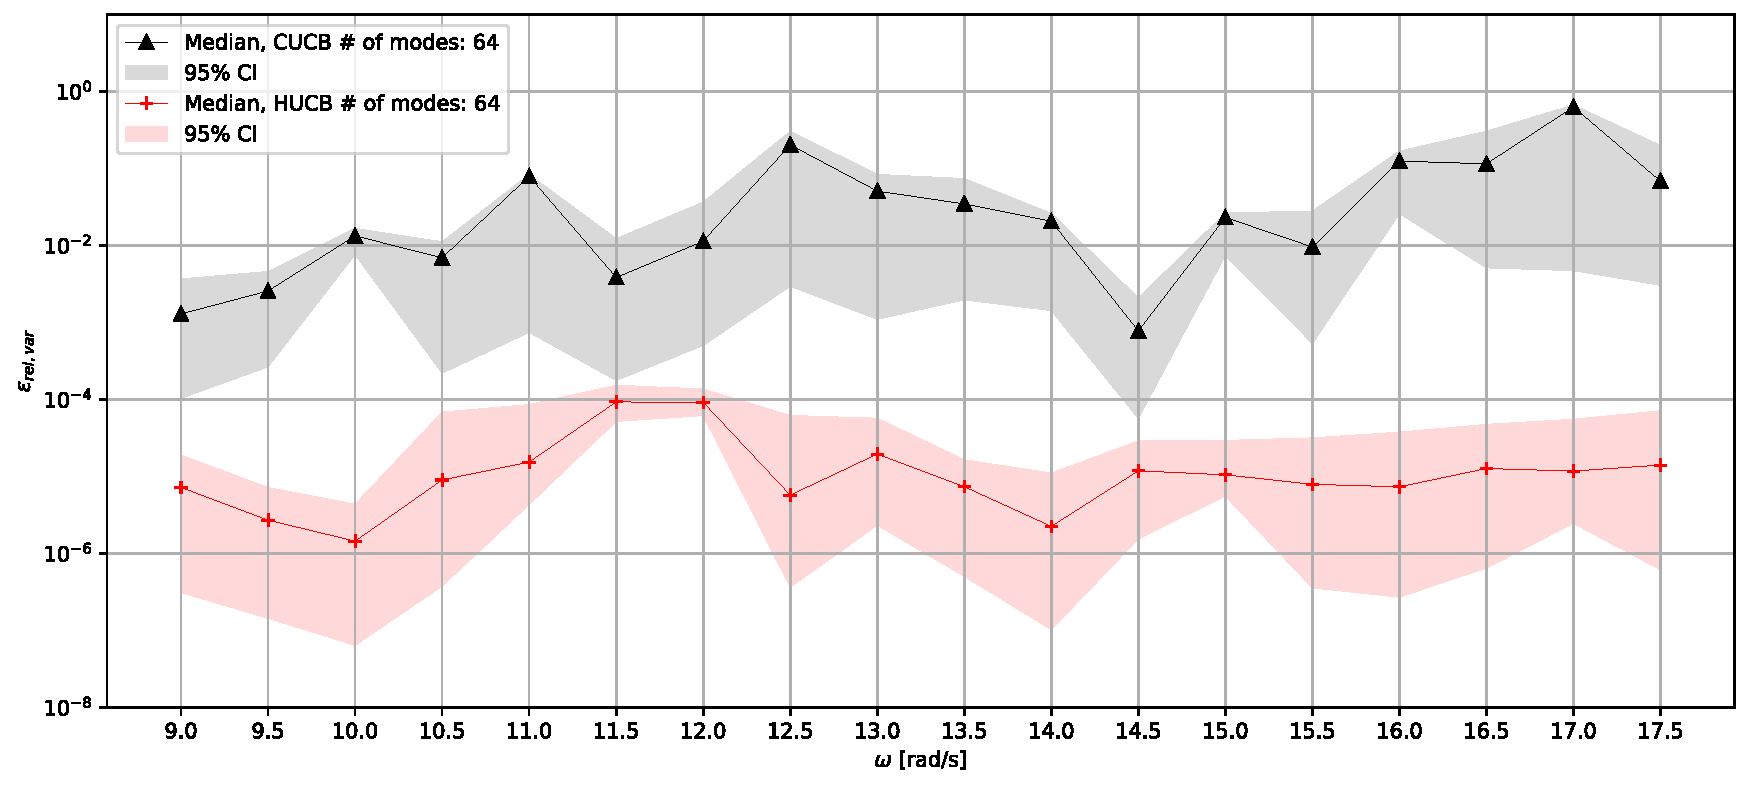
\includegraphics[width=1.0\textwidth]{
        plots/substructuring/plot_7.pdf
    }
    \caption{%
        Relative Variance Errors of $H_{AA}$ for The CUCB and HUCB Methods
    }
    \label{e_var HUCB_A_A}
\end{figure}
The two figures above show that while the relative mean errors from the two approaches are comparable, the HUCB method better approximates the FRFs' variabilities, thus leading to lower overall relative empirical error.
% -----------------------------------------------------------------------------
% Master thesis in the study program computational mechanics
%
% B.Sc. Rezha Adrian Tanuharja - 03751261
% M.Sc. Felix Schneider (supervisor)
%
% chapters/discussion/substructuring/point_B.tex
% Last edited 03 November 2023
% -----------------------------------------------------------------------------

\subsection{Vertical Acceleration at Node B}
\label{ssec: cms point B}

Figures \ref{FRF_MC_B_A_linear} and \ref{FRF_MC_B_A_log} show the vertical acceleration magnitudes at node B when a unit vertical force is present at node A.
\begin{figure}[H]
    \centering
    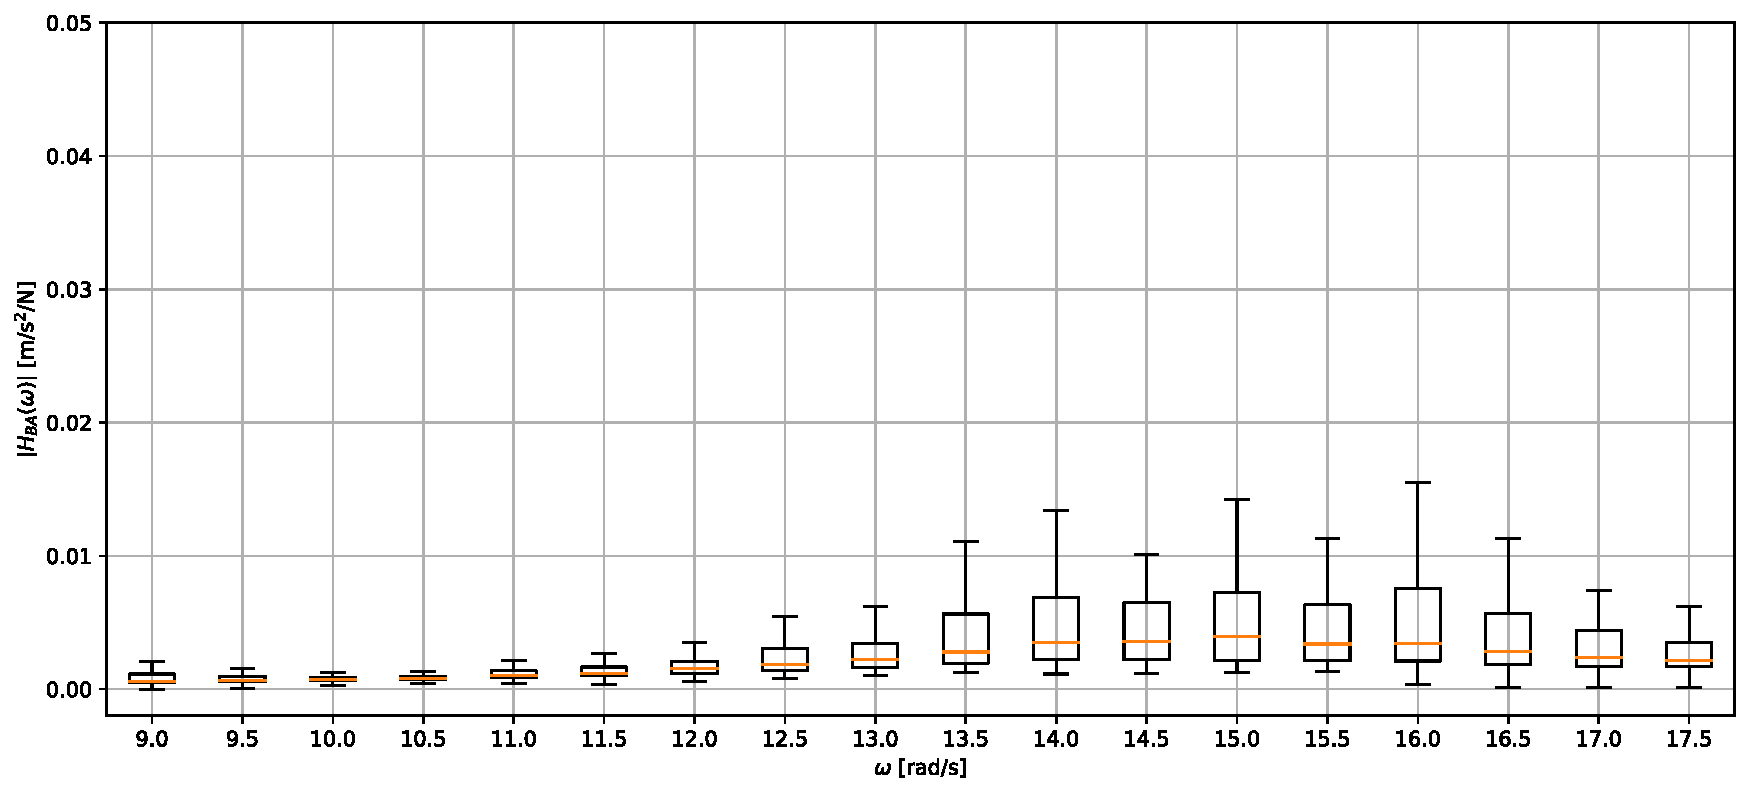
\includegraphics[width=1.0\textwidth]{
        plots/substructuring/plot_8_linear.pdf
    }
    \caption{%
        $\left|H_{BA}\right|$ from Direct MCS of The Complete Plate Model
    }
    \label{FRF_MC_B_A_linear}
\end{figure}
\begin{figure}[H]
    \centering
    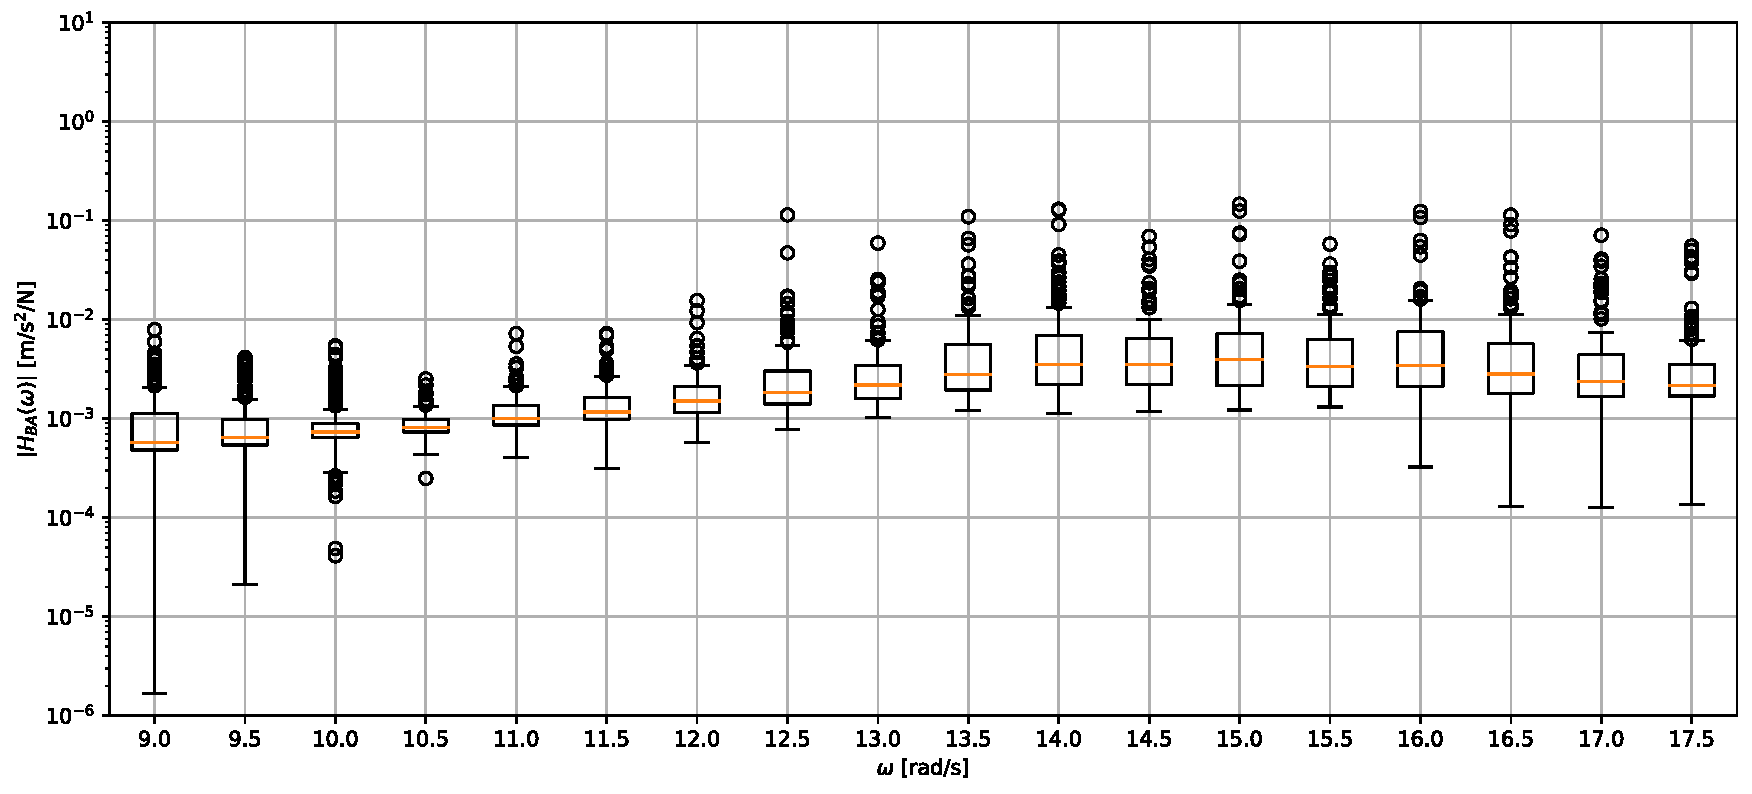
\includegraphics[width=1.0\textwidth]{
        plots/substructuring/plot_8_log.pdf
    }
    \caption{%
        $\left|H_{BA}\right|$ from Direct MCS of The Complete Plate Model with Outliers
    }
    \label{FRF_MC_B_A_log}
\end{figure}
Figure \ref{e_emp CUCB_B_A} shows the median relative empirical errors for the FRFs in each frequency in the above range using three different numbers of internal modes.
The figure exhibits a similar trend with figure \ref{e_emp CUCB_A_A}: as the number of internal modes increases, the relative empirical errors decrease.
\begin{figure}[H]
    \centering
    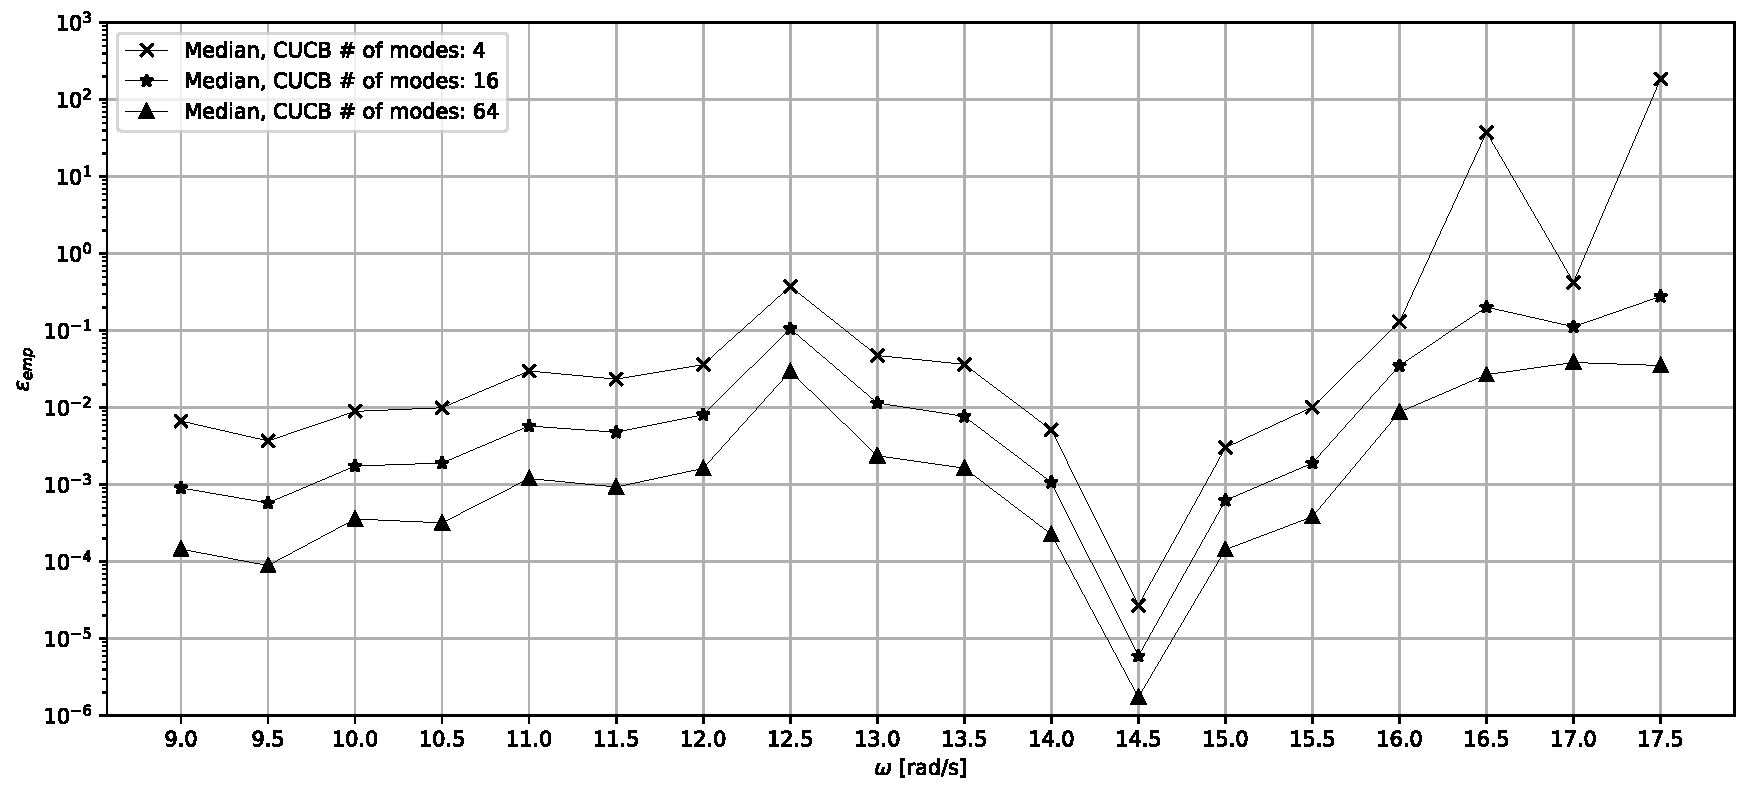
\includegraphics[width=1.0\textwidth]{
        plots/substructuring/plot_9.pdf
    }
    \caption{%
        Relative Empirical Errors of $H_{BA}$ for The CUCB Method
    }
    \label{e_emp CUCB_B_A}
\end{figure}

Figure \ref{e_emp HUCB_B_A} shows the medians and $95\%$ confidence intervals of the relative empirical errors of the FRFs' magnitudes for the crude and hybrid UCB methods.
\begin{figure}[H]
    \centering
    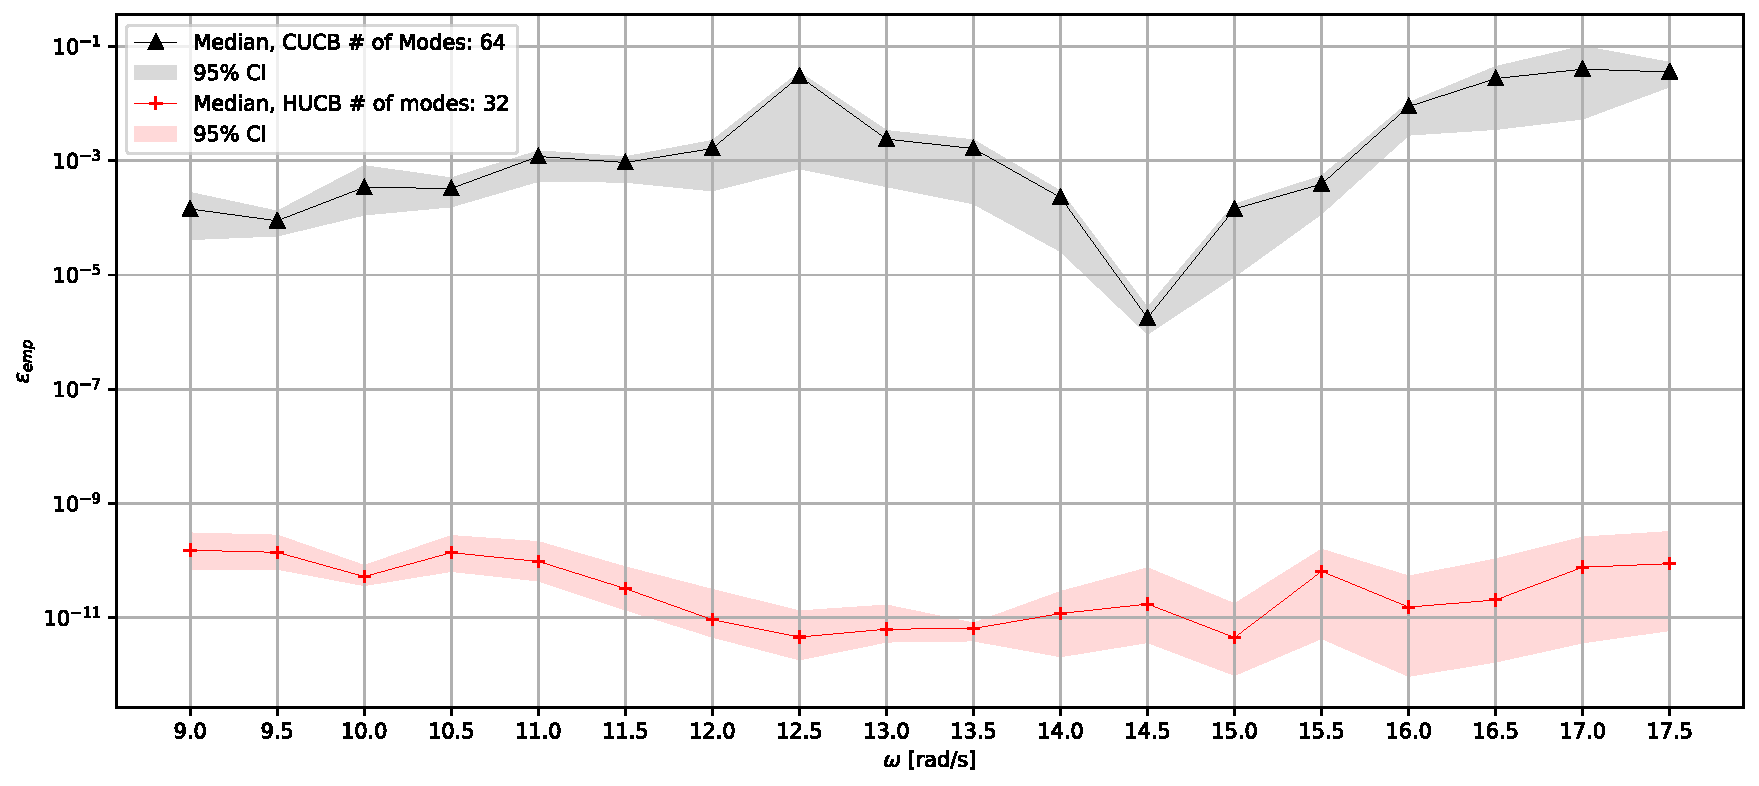
\includegraphics[width=1.0\textwidth]{
        plots/substructuring/plot_10.pdf
    }
    \caption{%
        Relative Empirical Errors of $H_{BA}$ for The CUCB and HUCB Methods
    }
    \label{e_emp HUCB_B_A}
\end{figure}
Comparing figure \ref{e_emp HUCB_A_A} with figure \ref{e_emp HUCB_B_A}, the benefit of the HUCB method over the CUCB method is more pronounced when the force and the response are at two different points or two different components.

Figure \ref{e_mean CUCB_B_A} shows the median relative mean errors of the FRFs' magnitudes for the CUCB method using three different numbers of internal modes.
\begin{figure}[H]
    \centering
    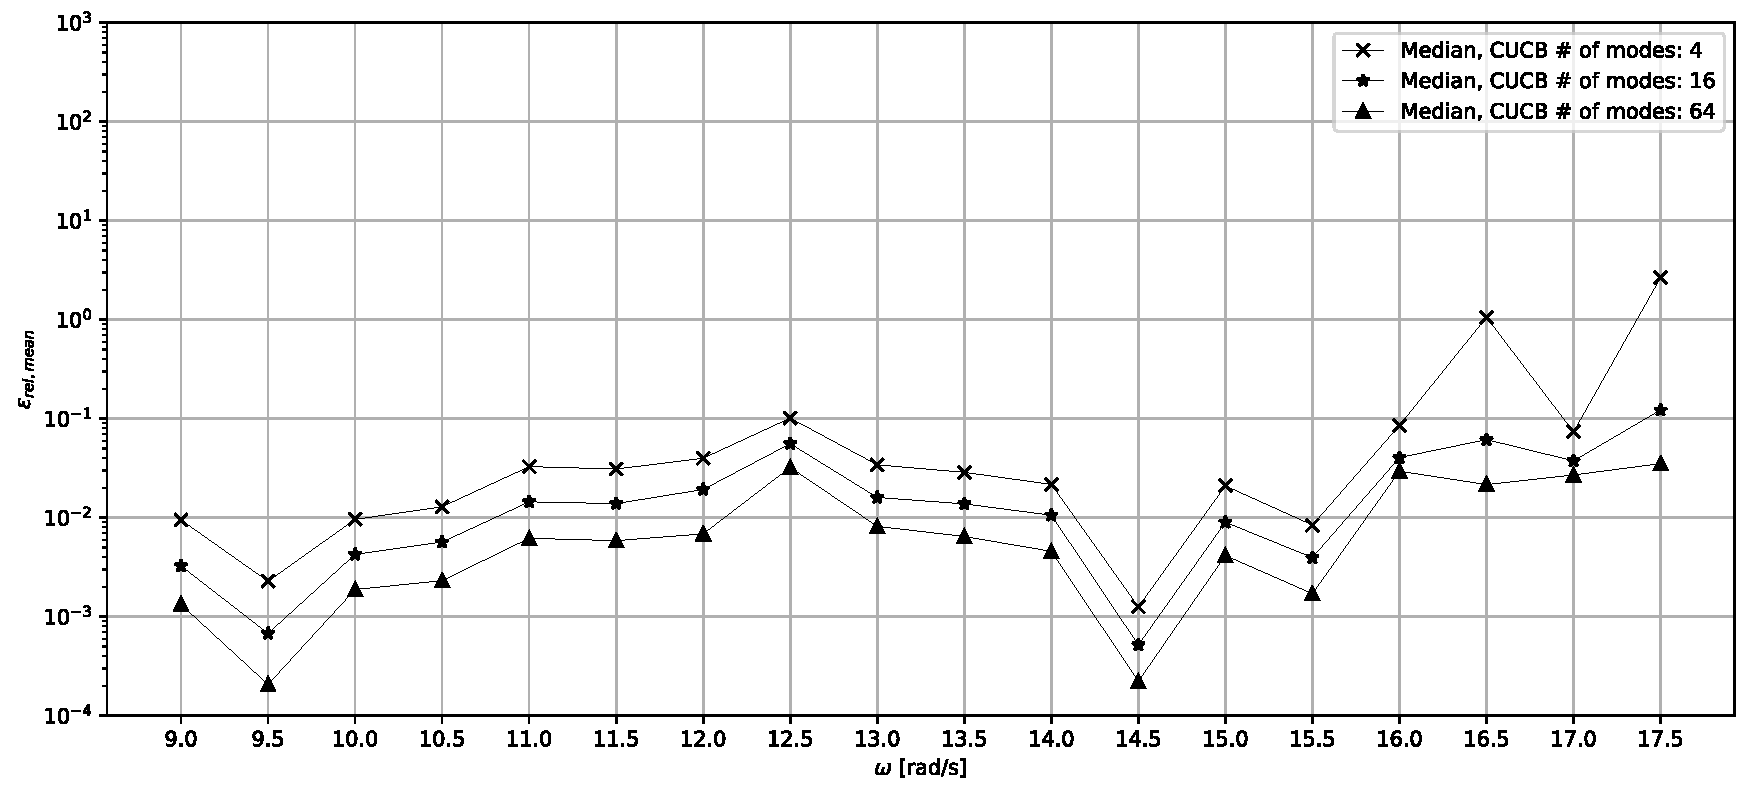
\includegraphics[width=1.0\textwidth]{
        plots/substructuring/plot_11.pdf
    }
    \caption{%
        Relative Mean Errors of $\left|H_{BA}\right|$ for The CUCB Method
    }
    \label{e_mean CUCB_B_A}
\end{figure}
Figure \ref{e_var CUCB_B_A} shows the median relative variance errors of the FRFs' magnitudes for the CUCB method using three different numbers of internal modes.
\begin{figure}[H]
    \centering
    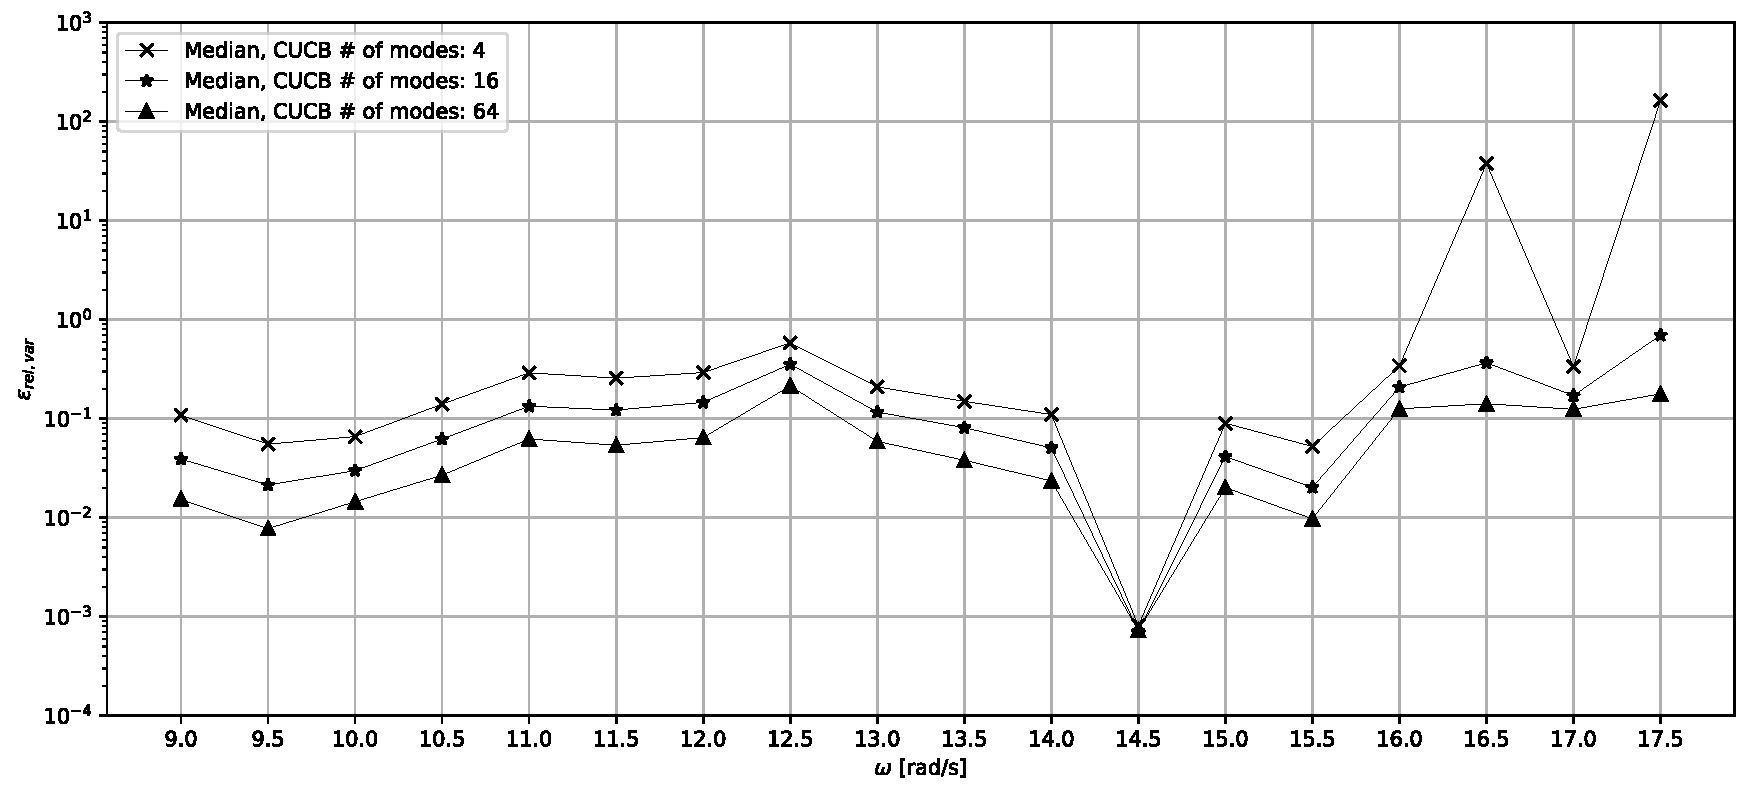
\includegraphics[width=1.0\textwidth]{
        plots/substructuring/plot_12.pdf
    }
    \caption{%
        Relative Variance Errors of $H_{BA}$ for The CUCB Method
    }
    \label{e_var CUCB_B_A}
\end{figure}
The two figures above exhibit similar trends with figure \ref{e_emp CUCB_B_A}: the relative mean errors decrease as the number of internal modes increases.
Overall, the relative mean errors are lower than the relative variance errors.

Figure \ref{e_mean HUCB_B_A} shows the medians and $95\%$ confidence intervals of the relative mean errors for the crude and hybrid UCB methods.
\begin{figure}[H]
    \centering
    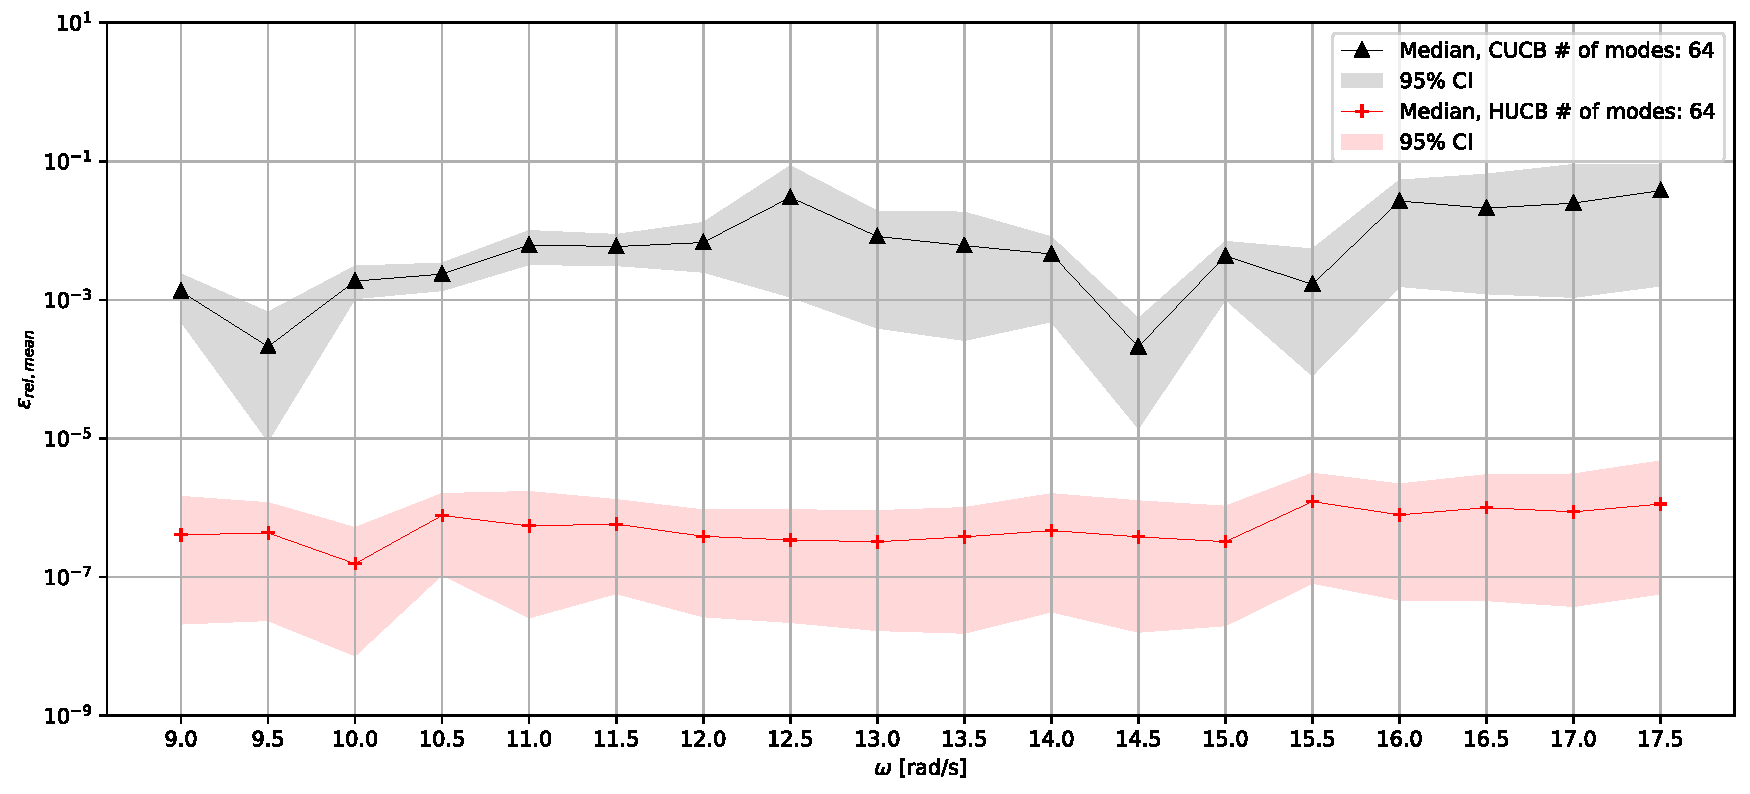
\includegraphics[width=1.0\textwidth]{
        plots/substructuring/plot_13.pdf
    }
    \caption{%
        Relative Mean Errors of $\left|H_{BA}\right|$ for The CUCB and HUCB Methods
    }
    \label{e_mean HUCB_B_A}
\end{figure}
Figure \ref{e_var HUCB_B_A} shows the medians and $95\%$ confidence intervals of the relative variance errors for the crude and hybrid UCB methods.
\begin{figure}[H]
    \centering
    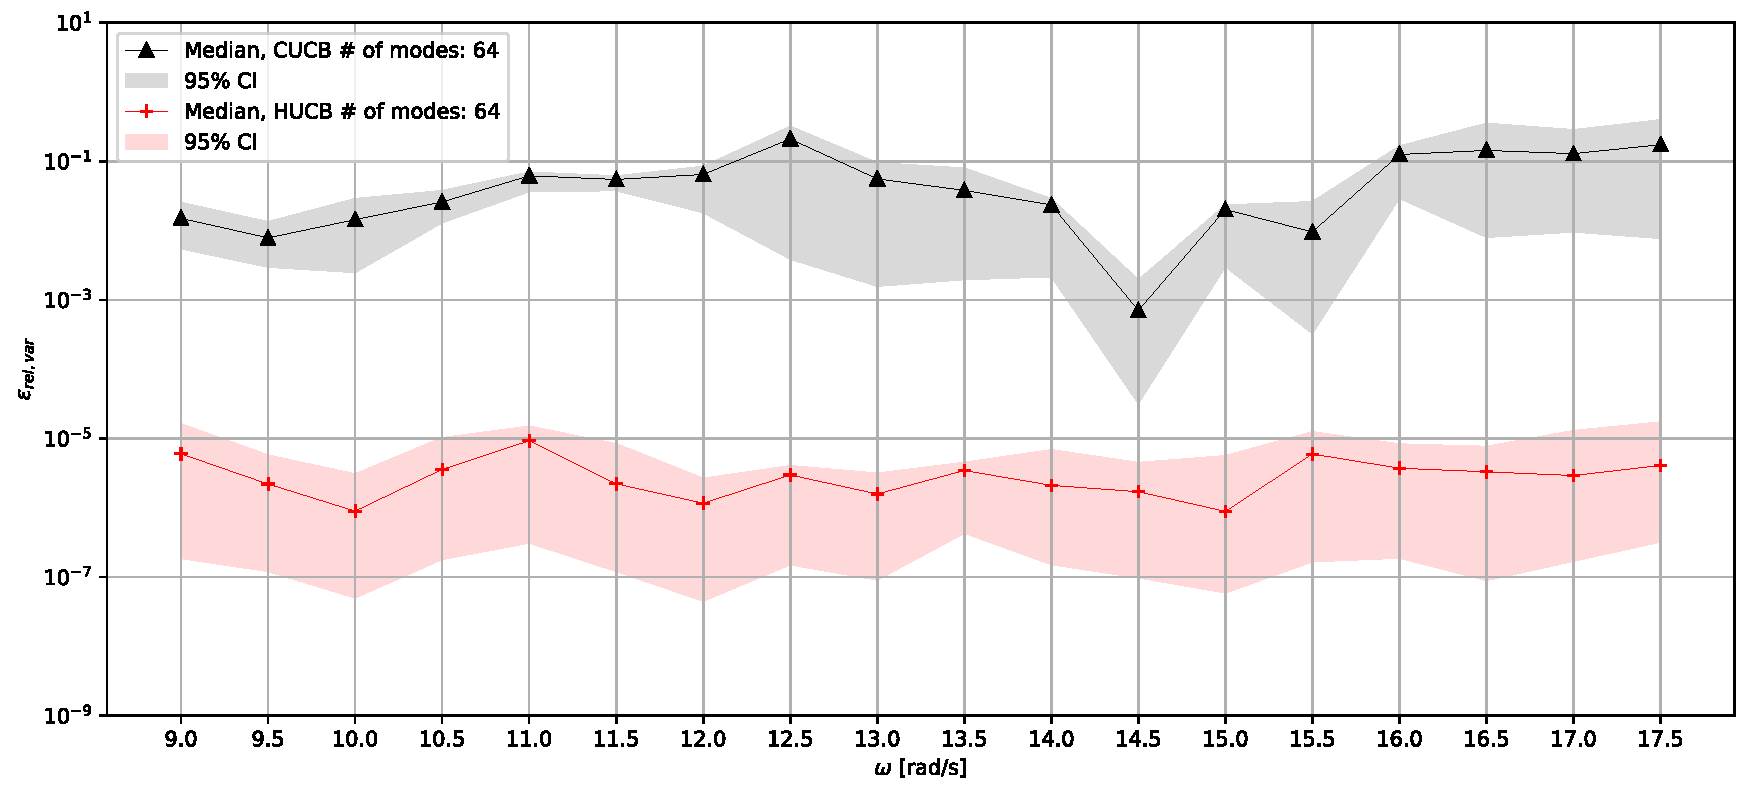
\includegraphics[width=1.0\textwidth]{
        plots/substructuring/plot_14.pdf
    }
    \caption{%
        Relative Variance Errors of $H_{BA}$ for The CUCB and HUCB Methods
    }
    \label{e_var HUCB_B_A}
\end{figure}
The two figures above show that both the relative mean errors and relative variance errors are lower when using the hybrid UCB method by several orders of magnitude.
% -----------------------------------------------------------------------------
% Master thesis in the study program computational mechanics
%
% B.Sc. Rezha Adrian Tanuharja - 03751261
% M.Sc. Felix Schneider (supervisor)
%
% chapters/literature/stochastic.tex
% Last edited 03 November 2023
% -----------------------------------------------------------------------------

\section{Uncertainty Propagation}
\label{sec: stochastic}

The previous section considers deterministic dynamic structures, i.e., it assumes that all structural parameters are precisely known.
This assumption is not necessarily valid.
{Alternatively, one can use a dynamic model with parametric uncertainties instead:}%
\begin{equation}
    \mathbf{D} \left(\omega, \mathbf{\Xi}\right)
    \mathbf{U} \left(\omega, \mathbf{\Xi}\right)
    =
    \mathbf{F} \left(\omega, \mathbf{\Xi}\right),
    \label{stochastic_eq_of_motion}
\end{equation}
where the dynamic stiffness, force vector, and displacement vector are functions of a set of zero-mean random variables $\mathbf{\Xi}=\left\{\xi_{1}, \xi_{2},...,\xi_{m}\right\}$.
In this context, the outputs of the model are not deterministic.
Therefore, the aim is to estimate the probabilistic characteristics of the model's outputs.

% -----------------------------------------------------------------------------
% Master thesis in the study program computational mechanics
%
% B.Sc. Rezha Adrian Tanuharja - 03751261
% M.Sc. Felix Schneider (supervisor)
%
% chapters/literature/stochastic/monteCarlo.tex
% Last edited 03 November 2023
% -----------------------------------------------------------------------------

\subsection{Monte Carlo Method}
\label{ssec: MC method}

The MC method is a classic uncertainty quantification approach.
It involves generating random samples of $\mathbf{\Xi}$, evaluating the model for each realization, and aggregating the results to estimate the probabilistic characteristics of the model outputs.
Algorithm \ref{alg: MC method} illustrates an MC simulation (MCS) for an uncertainty quantification of FRFs.
\input{algorithms/monteCarlo}
% -----------------------------------------------------------------------------
% Master thesis in the study program computational mechanics
%
% B.Sc. Rezha Adrian Tanuharja - 03751261
% M.Sc. Felix Schneider (supervisor)
%
% algorithm/PCE.tex
% Last edited 03 November 2023
% -----------------------------------------------------------------------------

\begin{center}
\begin{algorithm}[H]
    \label{alg: PCE}
    \ForEach{$\omega$ in $\left\{\omega_{1}, ..., \omega_{m}\right\}$}{
        \vspace{1.0em}%
        $\mathbf{Y} \longleftarrow [\phantom{x}]$ \\ 
        $\mathbf{A} \longleftarrow [\phantom{x}]$ \\ 
        \vspace{1.0em}%
        \tcp{Generate random samples}
        \For{$i = 1, ..., N_{sample}$}{
            $\mathbf{\Xi}_{i} \longleftarrow$
            \sample{$\mathbf{\Xi}$} \\
            \vspace{1.0em}%
            \tcc{Compute dynamic stiffness matrix $\mathbf{D}\left(\omega, \mathbf{\Xi}_{i}\right)$}
            $\dots$ \\
            \vspace{1.0em}%
            $
                \mathbf{Y}\left[i\right] \longleftarrow
                -\omega^{2}\left(\mathbf{D}\left(\omega, \mathbf{\Xi}_{i}\right)\right)^{-1}
            $ \\
            $
                \mathbf{A}\left[i\right] \longleftarrow
                \left[\Psi_{k}\left(\mathbf{\Xi}_{i}\right),\;\; k \in S\right]
            $
        }
        \vspace{1.0em}%
        $\left\{\mathbf{H}_{k}, k\in S\right\} \longleftarrow$ 
        \lsRegression{$\mathbf{Y}, \mathbf{A}$} \\
        \vspace{1.0em}%
        $\hat{\mathbf{H}} \longleftarrow [\phantom{x}]$ \\ 
        \vspace{1.0em}%
        \tcp{Perform MC simulation using PCE}
        \For{$i = 1, ..., N_{mcs}$}{
            $\mathbf{\Xi}_{i} \longleftarrow$
            \sample{$\mathbf{\Xi}$} \\
            \vspace{1.0em}%
            \tcp{Approximate FRF}
            $
                \hat{\mathbf{H}}\left[i\right] \longleftarrow
            $
                \sum{
                    $
                    \Psi_{k} \left(\mathbf{\Xi}_{i}\right)
                    \cdot 
                    \mathbf{H}_{k}
                    $
                }
            % $
        }
        \vspace{1.0em}%
        \tcc{Estimate characteristics of $\mathbf{H}\left(\omega, \mathbf{\Xi}\right)$ from $\hat{\mathbf{H}}$}
        $\dots$
    }
  \caption{Monte Carlo Simulation of The FRFs with PCE}
\end{algorithm}
\end{center}
% -----------------------------------------------------------------------------
% Master thesis in the study program computational mechanics
%
% B.Sc. Rezha Adrian Tanuharja - 03751261
% M.Sc. Felix Schneider (supervisor)
%
% chapters/literature/stochastic/sparsePCE.tex
% Last edited 03 November 2023
% -----------------------------------------------------------------------------

\subsection{Sparse PCE Model}
\label{ssec: sparse PCE}

The computation of FRFs is likely the most expensive step in the method above.
Therefore, the number of samples dictates the overall computational cost.
As the number of basis functions in the approximation increases, so does the required number of samples.
There are several procedures to shrink the number of basis functions.
The following is an example of such procedures and is a simplified version of the one in \cite{blatman2010adaptive}.

The procedure starts with an empty approximation.
It enriches the model with one basis function at a time and checks its accuracy.
If accuracy improves significantly, it keeps the basis function in the model.
Otherwise, it removes the basis functions from the model.
These steps aim to include only the basis functions that significantly improve the model's approximation.
Algorithm \ref{alg: sparse PCE addition} illustrates these steps.

\input{algorithms/sparsePCEAddition}

Subsequently, the procedure removes one basis function at a time from the approximation and checks the accuracy.
If accuracy declines significantly, it reinstates the basis in the approximation.
These steps aim to remove the basis functions that do not significantly improve the model's approximation.
Algorithm \ref{alg: sparse PCE removal} illustrates these steps.

\input{algorithms/sparsePCERemoval}

After the selective inclusion and exclusion steps above, only some of the basis functions are present in the PCE model.
Hence the term sparse PCE model.
% -----------------------------------------------------------------------------
% Master thesis in the study program computational mechanics
%
% B.Sc. Rezha Adrian Tanuharja - 03751261
% M.Sc. Felix Schneider (supervisor)
%
% chapters/literature/stochastic/RPCE.tex
% Last edited 03 November 2023
% -----------------------------------------------------------------------------

\subsection{Rational PCE Model}
\label{ssec: RPCE}

PCE requires a large number of basis functions to accurately represent the highly nonlinear behavior of FRFs near the structure's eigenfrequencies.
As the subsection above mentions, the large number of basis functions leads to a large number of required samples, thus increasing the overall computational cost.
{An alternative is approximating FRFs with ratios of PCEs:}%
\begin{equation}
    H_{pq} \left( \omega, \mathbf{\Xi} \right)
    \approx
    \frac{
        \sum_{k\in S_{u}}{
            u_{pqk}\left(\omega\right)
            \cdot
            \Psi_{k} \left( \mathbf{\Xi} \right)
        }
    }{
        \sum_{l\in S_{v}}{
            v_{pql}\left(\omega\right)
            \cdot
            \Psi_{l} \left( \mathbf{\Xi} \right)
        }
    }
    \quad
    S_{u} = \left\{1, ..., N_{u}\right\},
    \;
    S_{v} = \left\{1, ..., N_{v}\right\}
    .
    \label{RPCE_approx}
\end{equation}
The mean square error is typically the prime candidate to be an objective function in a linear regression problem.
However, the rational form of RPCE makes finding its minima less trivial.
{In \cite{schneider2020polynomial}, the authors define an alternative objective function for the minimization problem:}%
\begin{equation}
    \left\{
        \mathbf{u}_{pq},
        \mathbf{v}_{pq}
    \right\}
    =
    \underset{
        \left\{
            \hat{\mathbf{u}},
            \hat{\mathbf{v}}
        \right\}
        \in 
        \mathbb{C}^{N_{u}+N_{v}}
    }{\arg\min}
    \;
    \frac{1}{N}
    \sum_{i=0}^{N}
    \left\|
        H_{pq} \left( \mathbf{\Xi}_{i} \right)
        \cdot
        \sum_{l\in S_{v}}{
            \hat{v}_{l} \Psi_{l} \left( \mathbf{\Xi}_{i} \right)
        }
        -
        \sum_{k\in S_{u}}{
            \hat{u}_{k} \Psi_{k} \left( \mathbf{\Xi}_{i} \right)
        }
    \right\|_{2}^{2},
\end{equation}
where the dependency on frequency is intentionally missing to keep it concise.
{Subsequently, they show that the solution satisfies}%
\begin{equation}
    \begin{bmatrix}
        \mathbf{\Psi}_{U}^{T}
        \mathbf{\Psi}_{U}
        &
        -\mathbf{\Psi}_{U}^{T}
        \mathbf{M}
        \mathbf{\Psi}_{V}
        \\
        -\mathbf{\Psi}_{V}^{T}
        \mathbf{M}^{H}
        \mathbf{\Psi}_{U}
        &
        \mathbf{\Psi}_{V}^{T}
        \mathbf{M}^{H}
        \mathbf{M}
        \mathbf{\Psi}_{V}
    \end{bmatrix}
    \begin{pmatrix}
        \mathbf{u}_{pq} \\
        \mathbf{v}_{pq}
    \end{pmatrix}
    =
    \begin{pmatrix}
        \mathbf{0} \\
        \mathbf{0}
    \end{pmatrix},
    \label{SVD problem}
\end{equation}
{where}%
\begin{equation}
    \left[\mathbf{\Psi}_{U}\right]_{ij}
    =
    \Psi_{j} \left(\mathbf{\Xi}_{i}\right)
    \quad
    \forall
    \quad
    (i,j)\in\left\{1, ..., N\right\} \otimes
    \left\{1, ..., N_{u}\right\},
\end{equation}
\vspace{-3.0em}
\begin{equation}
    \left[\mathbf{\Psi}_{V}\right]_{ij}
    =
    \Psi_{j} \left(\mathbf{\Xi}_{i}\right)
    \quad
    \forall
    \quad
    (i,j)\in\left\{1, ..., N\right\} \otimes
    \left\{1, ..., N_{v}\right\},
\end{equation}
{and}%
\begin{equation}
    \mathbf{M}
    =
    \text{diag} \left(
        H_{pq} \left( \mathbf{\Xi}_{1} \right),
        H_{pq} \left( \mathbf{\Xi}_{2} \right),
        ..., 
        H_{pq} \left( \mathbf{\Xi}_{N} \right)
    \right).
\end{equation}
% -----------------------------------------------------------------------------
% Master thesis in the study program computational mechanics
%
% B.Sc. Rezha Adrian Tanuharja - 03751261
% M.Sc. Felix Schneider (supervisor)
%
% chapters/development.tex
% Last edited 03 November 2023
% -----------------------------------------------------------------------------

\chapter{Development and Formulation}
\label{ch: development}

% -----------------------------------------------------------------------------
% Master thesis in the study program computational mechanics
%
% B.Sc. Rezha Adrian Tanuharja - 03751261
% M.Sc. Felix Schneider (supervisor)
%
% chapters/development/uncertainCB.tex
% Last edited 03 November 2023
% -----------------------------------------------------------------------------

\section{Uncertain CB Method}
\label{sec: UCB}

One usually uses the CB or ECB method for deterministic structures. 
The uncertain CB method (UCB) is a modified CB method to tackle models with varying input parameters.

% -----------------------------------------------------------------------------
% Master thesis in the study program computational mechanics
%
% B.Sc. Rezha Adrian Tanuharja - 03751261
% M.Sc. Felix Schneider (supervisor)
%
% algorithm/naiveUCB.tex
% Last edited 03 November 2023
% -----------------------------------------------------------------------------

\begin{center}
\begin{algorithm}[H]
    \label{alg: NUCB}
    \ForEach{$\omega$ in $\left\{\omega_{1}, ..., \omega_{m}\right\}$}{
        \vspace{1.0em}%
        \For{$j = 1, ..., N_{sample}$}{
            \vspace{1.0em}%
            $\mathbf{\Xi}_{j} \longleftarrow$
            \sample{$\mathbf{\Xi}$} \\
            \vspace{1.0em}%
            \tcc{
                Compute matrices
                $\mathbf{M}\left(\mathbf{\Xi}_{j}\right)$,
                $\mathbf{K}\left(\mathbf{\Xi}_{j}\right)$
            }
            $\dots$ \\
            \vspace{1.0em}%
            $\mathbf{T} \longleftarrow$
            \enhancedCB{%
            $\mathbf{M}\left(\mathbf{\Xi}_{j}\right)$, 
            $\mathbf{K}\left(\mathbf{\Xi}_{j}\right)$,
            $s_{i}$, $s_{b}$
            } \\
            \vspace{1.0em}%
            \tcc{%
                Reduce components using $\mathbf{T}$ and solve for 
                $\mathbf{H} \left(\omega, \mathbf{\Xi}_{j}\right)$
            }
            $\dots$
        }
        $\dots$
    }
  \caption{The Naive UCB Method for FRFs}
\end{algorithm}
\end{center}
% -----------------------------------------------------------------------------
% Master thesis in the study program computational mechanics
%
% B.Sc. Rezha Adrian Tanuharja - 03751261
% M.Sc. Felix Schneider (supervisor)
%
% algorithm/crudeUCB.tex
% Last edited 03 November 2023
% -----------------------------------------------------------------------------

\begin{center}
\begin{algorithm}[H]
    \label{alg: CUCB}
    \tcc{
        Compute matrices
        $\mathbf{M}\left(\mathbf{\Xi}_{0}\right)$,
        $\mathbf{K}\left(\mathbf{\Xi}_{0}\right)$
    }
    $\dots$ \\
    \vspace{1.0em}%
    $\mathbf{T}_{0} \longleftarrow$
    \craigBampton{
    $\mathbf{M}\left(\mathbf{\Xi}_{0}\right)$, 
    $\mathbf{K}\left(\mathbf{\Xi}_{0}\right)$,
    $s_{i}$, $s_{b}$
    } \\
    \vspace{1.0em}% 
    \ForEach{$\omega$ in $\left\{\omega_{1}, ..., \omega_{m}\right\}$}{
        \vspace{1.0em}%
        \For{$j = 1, ..., N_{sample}$}{
            \vspace{1.0em}%
            $\mathbf{\Xi}_{j} \longleftarrow$
            \sample{$\mathbf{\Xi}$} \\
            \vspace{1.0em}%
            \tcc{%
                Reduce components using $\mathbf{T}_{0}$ and solve for 
                $\mathbf{H} \left(\omega, \mathbf{\Xi}_{j}\right)$
            }
            $\dots$
        }
        $\dots$
    }
  \caption{The Crude UCB Method for FRFs}
\end{algorithm}
\end{center}
% -----------------------------------------------------------------------------
% Master thesis in the study program computational mechanics
%
% B.Sc. Rezha Adrian Tanuharja - 03751261
% M.Sc. Felix Schneider (supervisor)
%
% algorithm/hybridUCB.tex
% Last edited 03 November 2023
% -----------------------------------------------------------------------------

\begin{center}
\begin{algorithm}[H]
    \label{alg: HUCB}
    \vspace{1.0em}%
    \tcp{Compute reference normal modes}
    $\mathbf{\Xi}_{0} \:\longleftarrow \mathbf{0}$ \\
    $\mathbf{\Phi}_{n} \longleftarrow$
    \genEigSol{$
        \mathbf{M}_{ii}\left(\mathbf{\Xi}_{0}\right), 
        \mathbf{K}_{ii}\left(\mathbf{\Xi}_{0}\right)
    $} \\
    \vspace{1.0em}%
    \ForEach{$\omega$ in $\left\{\omega_{1}, ..., \omega_{m}\right\}$}{
        \vspace{1.0em}%
        $\mathbf{\Phi}_{d} \longleftarrow$
        \modeSelector{$
            \mathbf{\Phi}_{n}, \omega
        $} \\
        \vspace{1.0em}%
        \tcp{Generate random samples}
        \For{$i = 1, ..., N_{train}$}{
            \vspace{1.0em}%
            $\mathbf{\Xi}_{i} \longleftarrow$
            \sample{$\mathbf{\Xi}$} \\
            \vspace{1.0em}%
            \tcc{Compute dynamic stiffness matrix $\mathbf{D}\left(\omega, \mathbf{\Xi}_{i}\right)$}
            $\dots$ \\
            \vspace{1.0em}%
            $
                \tilde{\mathbf{\Phi}}_{c} \longleftarrow 
                -\left(
                    \mathbf{D}_{ii}\left(\omega, \mathbf{\Xi}\right)
                \right)^{-1}
                \mathbf{D}_{ib}\left(\omega, \mathbf{\Xi}\right)
            $ \\
            \vspace{1.0em}%
            $
                \mathbf{T} \;\longleftarrow
                \left[
                    \begin{bmatrix}
                        \mathbf{\Phi}_{d} &
                        \tilde{\mathbf{\Phi}}_{c}
                    \end{bmatrix}
                    \begin{bmatrix}
                        \phantom{x}\mathbf{0}\phantom{.} &
                        \mathbf{I}\phantom{x}
                    \end{bmatrix}
                \right]
            $ \\
        \vspace{1.0em}% 
            \tcc{%
                Reduce components with $\mathbf{T}$ and solve for 
                $\mathbf{H} \left(\omega, \mathbf{\Xi}_{j}\right)$
            }
            $\dots$
        }
        \vspace{1.0em}%
        \tcc{Further processes}
        $\dots$
    }
  \caption{The Hybrid UCB Method for FRFs}
\end{algorithm}
\end{center}
% -----------------------------------------------------------------------------
% Master thesis in the study program computational mechanics
%
% B.Sc. Rezha Adrian Tanuharja - 03751261
% M.Sc. Felix Schneider (supervisor)
%
% chapters/development/sparseRPCE.tex
% Last edited 03 November 2023
% -----------------------------------------------------------------------------

\section{Sparse RPCE Model}
\label{sec: stepwise RPCE}

The sparse PCE's main idea is to use as few basis functions as possible without compromising the ability to approximate the outputs.
The procedure in \ref{ssec: sparse PCE} achieves this by using only the basis functions that contribute significantly to the approximation's quality.
The following is an adaptation of this procedure for the RPCE models.

% -----------------------------------------------------------------------------
% Master thesis in the study program computational mechanics
%
% B.Sc. Rezha Adrian Tanuharja - 03751261
% M.Sc. Felix Schneider (supervisor)
%
% chapters/development/sparseRPCE/inclusionCriteria.tex
% Last edited 03 November 2023
% -----------------------------------------------------------------------------

\subsection{Basis Inclusion Criteria}
\label{ssec: inclusion criteria}

The inclusion or exclusion of the basis functions is based on their contribution to the approximation's quality.
A metric to quantify the approximation's quality is necessary to do this.
{This study uses the coefficient of determination:}%
\begin{equation}
    R^{2}
    =
    1 -
    \left(1-\frac{1}{n}\right)
    \cdot
    \frac{
        \left\|\mathbf{x}-\hat{\mathbf{x}}\right\|_{2}^{2}
    }{
        \left\|\mathbf{x}-\overline{\mathbf{x}}\right\|_{2}^{2}
    },
\end{equation}
where $\mathbf{x}$ is the actual model outputs, $\overline{\mathbf{x}}$ is the average of the model outputs, and $\hat{\mathbf{x}}$ is the approximation.
This study defines a model to be better than another if it has a higher coefficient of determination.
A perfect model, i.e., a model that can produce $\hat{\mathbf{x}}=\mathbf{x}$ has a coefficient of determination of unity.
% -----------------------------------------------------------------------------
% Master thesis in the study program computational mechanics
%
% B.Sc. Rezha Adrian Tanuharja - 03751261
% M.Sc. Felix Schneider (supervisor)
%
% chapters/development/sparseRPCE/crossValidation.tex
% Last edited 03 November 2023
% -----------------------------------------------------------------------------

\subsection{Cross Validation}
\label{ssec: cross validation}

A common problem of a collocation-based surrogate model is overfitting, i.e., approximating the outputs well on a given sample set but poorly everywhere else.
One possible mitigation is the cross-validation technique: one splits the sample set into a training and a test set, builds the surrogate model using the training set, and subsequently evaluates its approximation quality using the test set.

This study uses a particular class of cross-validation techniques: the leave-one-out cross-validation.
The procedure approximates an output realization using an RPCE model trained with all input realizations except one that is associated with that particular output.
Algorithm \ref{alg: looRPCE} illustrates this procedure.

\input{algorithms/looRPCE}
% -----------------------------------------------------------------------------
% Master thesis in the study program computational mechanics
%
% B.Sc. Rezha Adrian Tanuharja - 03751261
% M.Sc. Felix Schneider (supervisor)
%
% chapters/development/sparseRPCE/selectionProcedure.tex
% Last edited 03 November 2023
% -----------------------------------------------------------------------------

\subsection{Basis Selection Procedure}
\label{ssec: selection procedure}

The procedure starts with all basis functions in the numerator and denominator.
It removes a basis function from the numerator and evaluates the approximation's quality.
If the coefficient of determination significantly declines, the basis function returns to the model.
{This study defines a significant decline in the coefficient of determination as:}%
\begin{equation}
    R^{2} - R_{-}^{2} > \epsilon_{0} \cdot \left(1-R^{2}\right),
    \label{decline criteria}
\end{equation}
where $\epsilon_{0}$ is a tuning parameter, $R^{2}$ and $R_{-}^{2}$ are the coefficient of determinations before and after the basis removal, respectively.
The author repeats these steps for all basis functions in the numerator, from the highest order to the lowest order.
Algorithm \ref{alg: sparse RPCE numerator} illustrates this process.

\input{algorithms/sparseRPCENumerator}

After going through all of the basis functions in the numerator, the same procedure takes place for the denominator.
Algorithm \ref{alg: sparse RPCE denominator} illustrates this process.

\input{algorithms/sparseRPCEDenominator}
% -----------------------------------------------------------------------------
% Master thesis in the study program computational mechanics
%
% B.Sc. Rezha Adrian Tanuharja - 03751261
% M.Sc. Felix Schneider (supervisor)
%
% algorithm/integratedFramework.tex
% Last edited 03 November 2023
% -----------------------------------------------------------------------------

\begin{center}
\begin{algorithm}[H]
    \label{alg: integrated framework 1}
    \SetKwProg{ForEach}{foreach}{ do}{}
    \SetKwProg{For}{for}{ do}{}
    \mpiInit{} \\
    $\dots$ \\
    \vspace{1.0em}%
    \tcp{Compute reference normal modes}
    $\mathbf{\Xi}_{0} \:\:\longleftarrow \mathbf{0}$ \\
    $\mathbf{\Phi}_{n} \;\longleftarrow$
    \genEigSol{%
        $\mathbf{M} \left(\mathbf{\Xi}_{0}\right)$,
        $\mathbf{K} \left(\mathbf{\Xi}_{0}\right)$
    } \\
    \vspace{1.0em}%
    $\mathbf{H} \longleftarrow \left\{\phantom{x}\right\}$, 
    $\mathbf{A}_{u} \longleftarrow \left\{\phantom{x}\right\}$, 
    $\mathbf{A}_{v} \longleftarrow \left\{\phantom{x}\right\}$ \\
    \vspace{1.0em}%
    \ForEach{$\omega$ in $\left\{\omega_{1}, ..., \omega_{m}\right\}$}{
        \vspace{1.0em}%
        $\mathbf{\Phi}_{d} \longleftarrow$
        \modeSelector{$
            \mathbf{\Phi}_{n}, \omega
        $} \\
        \vspace{1.0em}%
        \tcp{Generate random samples}
        \For{$j = 1, ..., N_{sample}$}{
            \vspace{1.0em}%
            $\mathbf{\Xi}_{j} \longleftarrow$
            \sample{$\mathbf{\Xi}$} \\
            \vspace{1.0em}%
            \tcc{Compute dynamic stiffness matrix $\mathbf{D} = \mathbf{D}\left(\omega, \mathbf{\Xi}_{j}\right)$}
            $\dots$ \\
            \vspace{1.0em}%
            $%
                \tilde{\mathbf{\Phi}}_{c} \longleftarrow
                -\mathbf{D}_{ii}^{-1}
                \mathbf{D}_{ib}
            $ \\
            \vspace{1.0em}%
            \tcc{Use $\mathbf{\Phi}_{d}$ and $\tilde{\mathbf{\Phi}}_{c}$ to compute $\overline{\mathbf{D}}$ and $\overline{\mathbf{F}}$}
            $\dots$ \\
            \vspace{1.0em}%
            $
                \mathbf{S}_{B\text{local}} \longleftarrow
                \overline{\mathbf{D}}_{BB}
                -
                \overline{\mathbf{D}}_{Bd}
                \left(
                    \overline{\mathbf{D}}_{dd}
                \right)^{-1}
                \overline{\mathbf{D}}_{dB}
            $ \\
            $
                \mathbf{P}_{B\text{local}} \longleftarrow
                \overline{\mathbf{F}}_{B}
                -
                \overline{\mathbf{D}}_{Bd}
                \left(
                    \overline{\mathbf{D}}_{dd}
                \right)^{-1}
                \overline{\mathbf{F}}_{d}
            $ \\
            \vspace{1.0em}%
            $\dots$ \\
            \vspace{1.0em}%
        }
    }
  \caption{MC Simulation with The CB Method and Sparse RPCE}
\end{algorithm}
\end{center}

\begin{center}
\begin{algorithm}[H]
    \label{alg: integrated framework 2}
    \SetKwProg{ForEach}{}{}{end}
    \SetKwProg{For}{}{}{end}
    \vspace{-1.6em}
    \ForEach{}{
        \vspace{-1.5em}
        \For{}{
            \vspace{1.0em}%
            $\dots$ \\
            \vspace{1.0em}%
            \uIf{$rank==0$}{
                \vspace{1.0em}%
                $\mathbf{S}_{B} \longleftarrow$
                \mpiGather{$\mathbf{D}_{B\text{local}}$} \\
                $\mathbf{P}_{B} \longleftarrow$
                \mpiGather{$\mathbf{F}_{B\text{local}}$} \\
                \vspace{1.0em}%
                $\mathbf{U}_{B} \longleftarrow$
                    \sum{$\mathbf{D}_{B}$}$^{-1}$ 
                    \sum{$\mathbf{F}_{B}$}
                \\
                \mpiBroadcast{$\mathbf{U}_{B}$} \\
                \vspace{1.0em}%
            }
            \Else{
                \tcp{Do nothing}
            }
            \vspace{1.0em}%
            $
                \mathbf{X}_{d} \longleftarrow
                \overline{\mathbf{D}}_{dd}^{-1}
                \left(
                    \overline{\mathbf{F}}_{d}
                    -
                    \overline{\mathbf{D}}_{db}
                    \mathbf{U}_{b}
                \right)
            $ \\
            \vspace{1.0em}%
            $\hat{\mathbf{H}} \left[j\right] \longleftarrow$ \\
            \vspace{1.0em}%
            $
                \hat{\mathbf{A}}_{u} \left[j\right] \longleftarrow
                \left[
                    \mathbf{\Psi}_{k} \left(\mathbf{\Xi}_{j}\right),
                    k \;= 1, ..., N_{u}
                \right]
            $ \\
            $
                \hat{\mathbf{A}}_{v} \left[j\right] \longleftarrow
                \left[
                    \mathbf{\Psi}_{l} \;\left(\mathbf{\Xi}_{j}\right),
                    l \:\:= 1, ..., N_{v}
                \right]
            $ \\
            \vspace{1.0em}%
        }
        \vspace{1.0em}%
        $S_{u}, S_{v} \longleftarrow$
        \basisSelector{%
            $\hat{\mathbf{H}}$, 
            $\mathbf{A}_{u}$, 
            $\mathbf{A}_{v}$
        } \\
        $\mathbf{u}, \mathbf{v} \longleftarrow$
        \trainRPCE{%
            $\hat{\mathbf{H}}$, 
            $\mathbf{A}_{u}$, 
            $\mathbf{A}_{v}$,
            $S_{u}$,
            $S_{v}$
        } \\
        \vspace{1.0em}%
        $\hat{\mathbf{H}} \longleftarrow \left\{\phantom{x}\right\}$ \\
        \vspace{1.0em}%
        \SetKwProg{For}{for}{}{end}
        \For{$j = 1, ..., N_{mcs}$}{
                \vspace{1.0em}%
                $\mathbf{\Xi}_{j} \longleftarrow$
                \sample{$\mathbf{\Xi}$} \\
                \vspace{1.0em}%
                $\hat{\mathbf{H}} \left[j\right] \longleftarrow$
                \computeRPCE{%
                    $\mathbf{\Xi}_{j}$,
                    $S_{u}$,
                    $S_{v}$
                }
                \vspace{1.0em}%
        }
        \vspace{1.0em}%
        \tcc{Estimate characteristics of $\mathbf{H}\left(\omega, \mathbf{\Xi}\right)$ from $\hat{\mathbf{H}}$}
        $\dots$
    }
  \caption{MC Simulation with The CB Method and Sparse RPCE (Cont'd)}
\end{algorithm}
\end{center}
% -----------------------------------------------------------------------------
% Master thesis in the study program computational mechanics
%
% B.Sc. Rezha Adrian Tanuharja - 03751261
% M.Sc. Felix Schneider (supervisor)
%
% chapters/methodology.tex
% Last edited 03 November 2023
% -----------------------------------------------------------------------------

\chapter{Methodology}
\label{ch: methodology}

This study systematically evaluates the proposed framework's performance using a case study and by following a specific procedure.
In this section, the author details the case study, the evaluation procedure, as well as the error measure for performance quantification.

% -----------------------------------------------------------------------------
% Master thesis in the study program computational mechanics
%
% B.Sc. Rezha Adrian Tanuharja - 03751261
% M.Sc. Felix Schneider (supervisor)
%
% chapters/methodology/caseStudy.tex
% Last edited 03 November 2023
% -----------------------------------------------------------------------------

\section{Case Study}
\label{sec: case study}

This study demonstrates the practical application of the new framework using a simple yet relevant example: a plate clamped at both of its ends.
The choice of case is deliberate, as it is sufficiently large for the substructuring methods while still maintaining the feasibility of direct MC simulations.
Figure \ref{fig: case study} illustrates the plate and its dimensions.

% -----------------------------------------------------------------------------
% Master thesis in the study program computational mechanics
%
% B.Sc. Rezha Adrian Tanuharja - 03751261
% M.Sc. Felix Schneider (supervisor)
%
% chapters/methodology/caseStudy.tex
% Last edited 03 November 2023
% -----------------------------------------------------------------------------

\section{Case Study}
\label{sec: case study}

This study demonstrates the practical application of the new framework using a simple yet relevant example: a plate clamped at both of its ends.
The choice of case is deliberate, as it is sufficiently large for the substructuring methods while still maintaining the feasibility of direct MC simulations.
Figure \ref{fig: case study} illustrates the plate and its dimensions.

\input{images/caseStudy}

Table \ref{table: Plate Parameter} lists the relevant plate's parameters.
The plate's density and thickness are uncertain and modeled by random variables.
The parameters $\xi_{1}$ and $\xi_{2}$ are statistically independent standard normal random variables.

\begin{table}[H]
    \setlength{\extrarowheight}{2pt}
    \centering
    \begin{tabular}{
        L{0.32\textwidth}rccC{0.25\textwidth}
    }
        \hline
        Parameter & \multicolumn{3}{c}{Value} & Unit \\
        \hline
        Thickness &
            $(1.0+0.2\xi_{1})$ & $\times$ & $0.01$ &
            \einheit{m} \\
        Density & 
            $(1.0+0.2\xi_{2})$ & $\times$ & $7850.0$ &
            \einheit{kg/{m}^{3}} \\
        Shear modulus & 
            \multicolumn{3}{c}{$79.3$} &
            \einheit{GPa} \\
        Shear correction factor & 
            \multicolumn{3}{c}{$0.83$} &
            -- \\
        Poisson ratio & 
            \multicolumn{3}{c}{$0.3$} &
            -- \\
        \hline
    \end{tabular}
    \caption{Plate's Parameters in The Case Study}
    \label{table: Plate Parameter}
\end{table}

Two discrete models approximate the plate using the FE method with Kirchoff plate theory: the complete plate model and the substructured plate model.
The proposed framework uses the latter to generate training data for the NI-RPCE models, which will approximate the complete plate model.
On the other hand, the FRFs from direct MCS using the complete plate model serve as the baselines for comparison.

\input{chapters/methodology/caseStudy/completeModel}
\input{chapters/methodology/caseStudy/substructuredModel}
\input{chapters/methodology/caseStudy/surrogateModel}

Table \ref{table: Plate Parameter} lists the relevant plate's parameters.
The plate's density and thickness are uncertain and modeled by random variables.
The parameters $\xi_{1}$ and $\xi_{2}$ are statistically independent standard normal random variables.

\begin{table}[H]
    \setlength{\extrarowheight}{2pt}
    \centering
    \begin{tabular}{
        L{0.32\textwidth}rccC{0.25\textwidth}
    }
        \hline
        Parameter & \multicolumn{3}{c}{Value} & Unit \\
        \hline
        Thickness &
            $(1.0+0.2\xi_{1})$ & $\times$ & $0.01$ &
            \einheit{m} \\
        Density & 
            $(1.0+0.2\xi_{2})$ & $\times$ & $7850.0$ &
            \einheit{kg/{m}^{3}} \\
        Shear modulus & 
            \multicolumn{3}{c}{$79.3$} &
            \einheit{GPa} \\
        Shear correction factor & 
            \multicolumn{3}{c}{$0.83$} &
            -- \\
        Poisson ratio & 
            \multicolumn{3}{c}{$0.3$} &
            -- \\
        \hline
    \end{tabular}
    \caption{Plate's Parameters in The Case Study}
    \label{table: Plate Parameter}
\end{table}

Two discrete models approximate the plate using the FE method with Kirchoff plate theory: the complete plate model and the substructured plate model.
The proposed framework uses the latter to generate training data for the NI-RPCE models, which will approximate the complete plate model.
On the other hand, the FRFs from direct MCS using the complete plate model serve as the baselines for comparison.

% -----------------------------------------------------------------------------
% Master thesis in the study program computational mechanics
%
% B.Sc. Rezha Adrian Tanuharja - 03751261
% M.Sc. Felix Schneider (supervisor)
%
% chapters/methodology/caseStudy/completeModel.tex
% Last edited 03 November 2023
% -----------------------------------------------------------------------------

\subsection{Complete Plate Model}
\label{ssec: full model}

The discretization process uses biquadratic rectangular elements in a uniform mesh. There are three DOFs at each node: the vertical displacement, the rotation about the $x$ axis, and the rotation about the $y$ axis.
Tabel \ref{table: Mesh Parameter} provides the mesh's parameters.

\begin{table}[H]
    \setlength{\extrarowheight}{2pt}
    \centering 
    \begin{tabular}{
        L{0.3\textwidth} C{0.2\textwidth}
    }
        \hline
        Parameter & 
        Value \\
        \hline
        Number of elements (x) &
        48 \\
        Number of elements (y) &
        20 \\
        & \\
        Total number of nodes &
        3977 \\
        Total number of DOFs &
        11931 \\
        \hline 
    \end{tabular}
    \caption{Complete Plate Model Mesh's Parameters}
    \label{table: Mesh Parameter}
\end{table}%
%
The case study focuses on two particular nodes: node A located on the edge of the plate and node B located inside the plate's interior.
Table \ref{table: Node Coordinates} provides the coordinates of these two nodes.

\begin{table}[H]
    \setlength{\extrarowheight}{2pt}
    \centering
    \begin{tabular}{
        C{0.15\textwidth} C{0.15\textwidth} C{0.15\textwidth}
    }
        \hline
        Node & $x$ [m] & $y$ [m] \\
        \hline
        A & $5.\bar{3}$ & $4.0$ \\
        B & $1.\bar{3}$ & $1.9$ \\
        \hline
    \end{tabular}
    \caption{Coordinates of Two Nodes of Interest}
    \label{table: Node Coordinates}
\end{table}

In the evaluation, the author applies a unit vertical force on node A and computes the vertical accelerations of nodes A and B.
Figure \ref{fig: complete model} illustrates the meshed full plate model and the two nodes.

\input{images/completeModel}
% -----------------------------------------------------------------------------
% Master thesis in the study program computational mechanics
%
% B.Sc. Rezha Adrian Tanuharja - 03751261
% M.Sc. Felix Schneider (supervisor)
%
% images/substructuredModel.tex
% Last edited 03 November 2023
% -----------------------------------------------------------------------------

\begin{figure}[H]
    \centering

    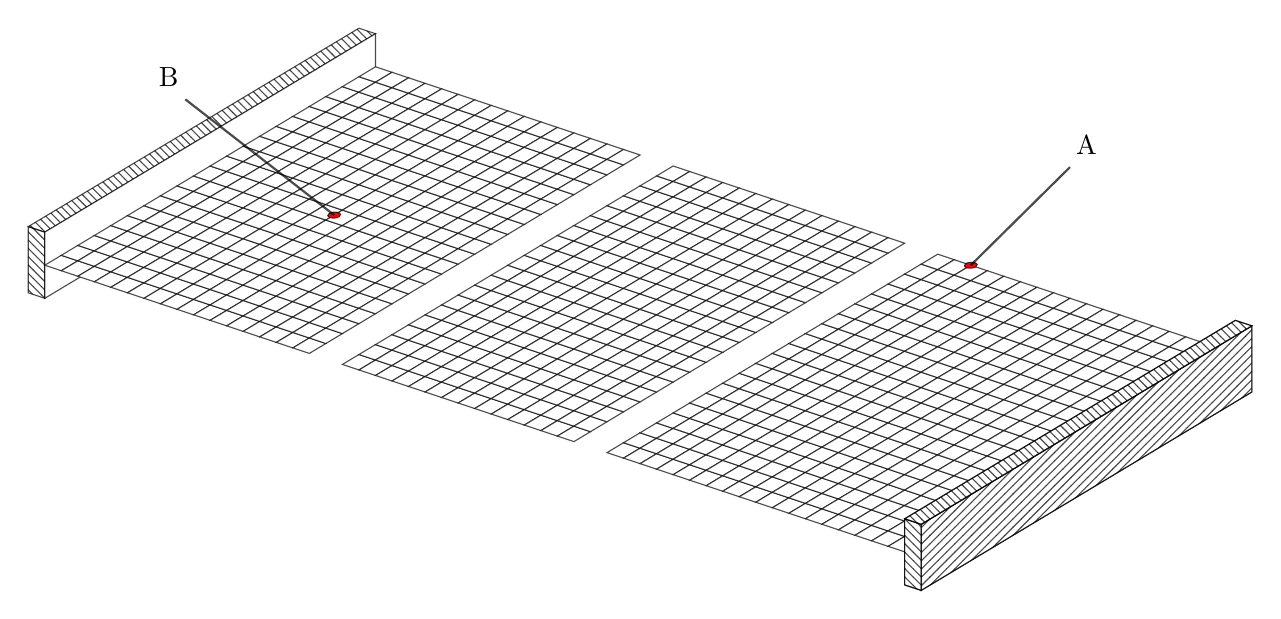
\begin{tikzpicture}[
        scale=0.35, 
        %
        % Isometric-esque appearance
        x={( 0.6cm,-0.2cm)}, 
        y={( 0.5cm, 0.3cm)}, 
        z={( 0.0cm, 1.0cm)}, 
        %
        draw opacity=0.7
    ]

        % Define the gap between the components
        \def\gap{2.0}

        % Define grid parameters
        % maxes are lengths - one step because of plotting
        \def\xmin{0.0} \def\xmax{15.0}
        \def\ymin{0.0} \def\ymax{22.8}

        % the dimension of each rectangular element
        \def\xstep{1.0}
        \def\ystep{1.2}

        % Define clamping wall parameters
        \def\wallh{1.2}
        \def\wallt{1.0}

        % Define markers' diameter
        \def\noder{0.5}

        % Draw the side left clamping wall 
        \draw[pattern=north west lines] 
            (   \xmin, \ymin, -\wallh) -- 
            (   \xmin, \ymin,  \wallh) -- 
            ( -\wallt, \ymin,  \wallh) -- 
            ( -\wallt, \ymin, -\wallh) -- 
            cycle;

        % Draw the top left clamping wall
        \draw[pattern=north west lines] 
            (   \xmin, \ymin       ,  \wallh) -- 
            (   \xmin, \ymax+\ystep,  \wallh) -- 
            ( -\wallt, \ymax+\ystep,  \wallh) -- 
            ( -\wallt, \ymin       ,  \wallh) -- 
            cycle;

        % Draw the front left clamping wall
        \draw[fill=white]
            (   \xmin, \ymin       , -\wallh) -- 
            (   \xmin, \ymax+\ystep, -\wallh) --
            (   \xmin, \ymax+\ystep,  \wallh) --
            (   \xmin, \ymin       ,  \wallh) -- 
            cycle; 
    
        % Draw the left component
        \foreach \x in {\xmin,\xstep,...,\xmax}
            \foreach \y in {\ymin,\ystep,...,\ymax}
                \draw[fill=white] 
                      ( \x   , \y   , 0) -- 
                    ++( \xstep, 0    , 0) -- 
                    ++( 0    , \ystep, 0) -- 
                    ++(-\xstep, 0    , 0) -- 
                    cycle;

        \def\xmax{13.0}
        \def\offset{16.0}
        \foreach \x in {\xmin,\xstep,...,\xmax}
            \foreach \y in {\ymin,\ystep,...,\ymax}
                \draw[fill=white] 
                      ( \x + \offset + \gap  , \y, 0) -- 
                    ++( \xstep, 0    , 0) -- 
                    ++( 0    , \ystep, 0) -- 
                    ++(-\xstep, 0    , 0) -- 
                    cycle;

        \def\xmax{17.0}
        \def\offset{30.0}
        \foreach \x in {\xmin,\xstep,...,\xmax}
            \foreach \y in {\ymin,\ystep,...,\ymax}
                \draw[fill=white] 
                      ( \x + \offset + 2*\gap  , \y, 0) -- 
                    ++( \xstep, 0    , 0) -- 
                    ++( 0    , \ystep, 0) -- 
                    ++(-\xstep, 0    , 0) -- 
                    cycle;

        % Put the back right clamping wall in front of the grid
        \def\offset{48.0}
        \draw[fill=white]
            ( \offset+\wallt+2*\gap, \ymin       , -\wallh) -- 
            ( \offset+\wallt+2*\gap, \ymax+\ystep, -\wallh) --
            ( \offset+\wallt+2*\gap, \ymax+\ystep,  \wallh) --
            ( \offset+\wallt+2*\gap, \ymin       ,  \wallh) -- 
            cycle; 

        % Draw the back right clamping wall
        \draw[pattern=north east lines]
            ( \offset+\wallt+2*\gap, \ymin       , -\wallh) -- 
            ( \offset+\wallt+2*\gap, \ymax+\ystep, -\wallh) --
            ( \offset+\wallt+2*\gap, \ymax+\ystep,  \wallh) --
            ( \offset+\wallt+2*\gap, \ymin       ,  \wallh) -- 
            cycle; 

        % Put the side right clamping wall in front of the grid
        \draw[fill=white] 
            ( \offset+2*\gap       , \ymin, -\wallh) -- 
            ( \offset+2*\gap       , \ymin,  \wallh) -- 
            ( \offset+2*\gap+\wallt, \ymin,  \wallh) -- 
            ( \offset+2*\gap+\wallt, \ymin, -\wallh) -- 
            cycle;
        
        % Draw the side right clamping wall
        \draw[pattern=north west lines] 
            ( \offset+2*\gap       , \ymin, -\wallh) -- 
            ( \offset+2*\gap       , \ymin,  \wallh) -- 
            ( \offset+2*\gap+\wallt, \ymin,  \wallh) -- 
            ( \offset+2*\gap+\wallt, \ymin, -\wallh) -- 
            cycle;
        
        % Put the top right clamping wall in front of the grid
        \draw[fill=white] 
            ( \offset+2*\gap       , \ymin       ,  \wallh) -- 
            ( \offset+2*\gap       , \ymax+\ystep,  \wallh) -- 
            ( \offset+2*\gap+\wallt, \ymax+\ystep,  \wallh) -- 
            ( \offset+2*\gap+\wallt, \ymin       ,  \wallh) -- 
            cycle;

        % Draw the top right clamping wall
        \draw[pattern=north west lines] 
            ( \offset+2*\gap       , \ymin       ,  \wallh) -- 
            ( \offset+2*\gap       , \ymax+\ystep,  \wallh) -- 
            ( \offset+2*\gap+\wallt, \ymax+\ystep,  \wallh) -- 
            ( \offset+2*\gap+\wallt, \ymin       ,  \wallh) -- 
            cycle;

        % Draw a marker for the node B
        \draw[fill=red] 
            ( 8*\xstep, 9.5*\ystep ) ellipse (0.3 and 0.3);
        % Draw a line pointing at the marker for the node B
        \draw[thick]
            (  8*\xstep, 9.5*\ystep,        0 ) --
            ( -1*\xstep, 9.5*\ystep, 2*\wallh );
        % Add label B
        \node at
            ( -2*\xstep, 9.5*\ystep, 2*\wallh+0.6*\xstep ) {B};

        % Draw a marker for the node A
        \draw[fill=red] 
            ( 32*\xstep+2*\gap, 20*\ystep ) ellipse (0.3 and 0.3);
        % Draw a line pointing at the two markers for the node A
        \draw[thick]
            ( 32*\xstep+2*\gap         , 20*\ystep       , 0               ) --
            ( 32*\xstep+  \gap+7*\xstep, 20*\ystep+\ystep, \wallh+3*\xstep );
        % Add label A
        \node at (32*\xstep+8*\xstep+\gap,20*\ystep+\ystep, \wallh+4*\xstep) {A};

    \end{tikzpicture}
    \caption{Meshed Substructured Plate Model with Locations of Nodes A and B}
    \label{fig: substructured model}
\end{figure}
% -----------------------------------------------------------------------------
% Master thesis in the study program computational mechanics
%
% B.Sc. Rezha Adrian Tanuharja - 03751261
% M.Sc. Felix Schneider (supervisor)
%
% chapters/methodology/caseStudy/surrogateModel.tex
% Last edited 03 November 2023
% -----------------------------------------------------------------------------

\subsection{Sparse NI-RPCE Model}
\label{ssec: surrogate model}

This study uses RPCE models with products of probabilist Hermite polynomials as the basis functions, as in \eqref{prob Hermite products}.
The numerator is a PCE with an order of $5$ while the denominator is a PCE with an order of $6$.
Therefore, the basis functions in the numerator and denominator satisfy
\begin{equation}
    \Psi_{k}\left(\mathbf{\Xi}\right)
    =
    {He}_{r_{k}} \left(\xi_{1}\right)
    \cdot
    {He}_{s_{k}} \left(\xi_{2}\right)
    \phantom{x}
    \forall 
    \phantom{x}
    r_{k}, s_{k} \in \mathbb{N}, 
    \phantom{x}
    r_{k} + s_{k} \leq 5
\end{equation}
and
\begin{equation}
    \Psi_{l}\left(\mathbf{\Xi}\right)
    =
    {He}_{r_{l}} \left(\xi_{1}\right)
    \cdot
    {He}_{s_{l}} \left(\xi_{2}\right)
    \phantom{x}
    \forall 
    \phantom{x}
    r_{l}, s_{l} \in \mathbb{N}, 
    \phantom{x}
    r_{l} + s_{l} \leq 6,
\end{equation}
respectively.
The author obtains the coefficient in \eqref{RPCE_approx} by solving \eqref{SVD problem}.
There are $49$ basis functions in the numerator and denominator of the RPCE models.
The author reduces the number of basis functions by following the algorithms \ref{alg: sparse RPCE numerator} and \ref{alg: sparse RPCE denominator} with $\epsilon_{0}=1.0$.
% -----------------------------------------------------------------------------
% Master thesis in the study program computational mechanics
%
% B.Sc. Rezha Adrian Tanuharja - 03751261
% M.Sc. Felix Schneider (supervisor)
%
% chapters/methodology/testProcedure.tex
% Last edited 03 November 2023
% -----------------------------------------------------------------------------

\section{Evaluation Procedures}
\label{sec: evaluation procedure}

First, the author evaluates the performance of CUCB and HUCB in approximating the complete plate model.
The author generates an experimental design (ED) of size $N_{ed}=300$ through random sampling.
Subsequently, a direct MCS for FRFs using the complete plate model takes place.
The outputs serve as the benchmark for comparison.
Then, the author runs MCS for FRFs using the substructured plate model with the CUCB and HUCB methods.
Comparisons between the outputs with the benchmark and error calculations follow.
Because the size of the ED is not large, the author uses bootstrapping with a $1000$ number of resamplings to estimate the error statistics.
Figure \ref{flowchart: UCB procedure} illustrates this evaluation procedure.
% -----------------------------------------------------------------------------
% Master thesis in the study program computational mechanics
%
% B.Sc. Rezha Adrian Tanuharja - 03751261
% M.Sc. Felix Schneider (supervisor)
%
% images/procedureUCB.tex
% Last edited 03 November 2023
% -----------------------------------------------------------------------------

\begin{figure}[H]
    \centering
    \scalebox{0.75}{
        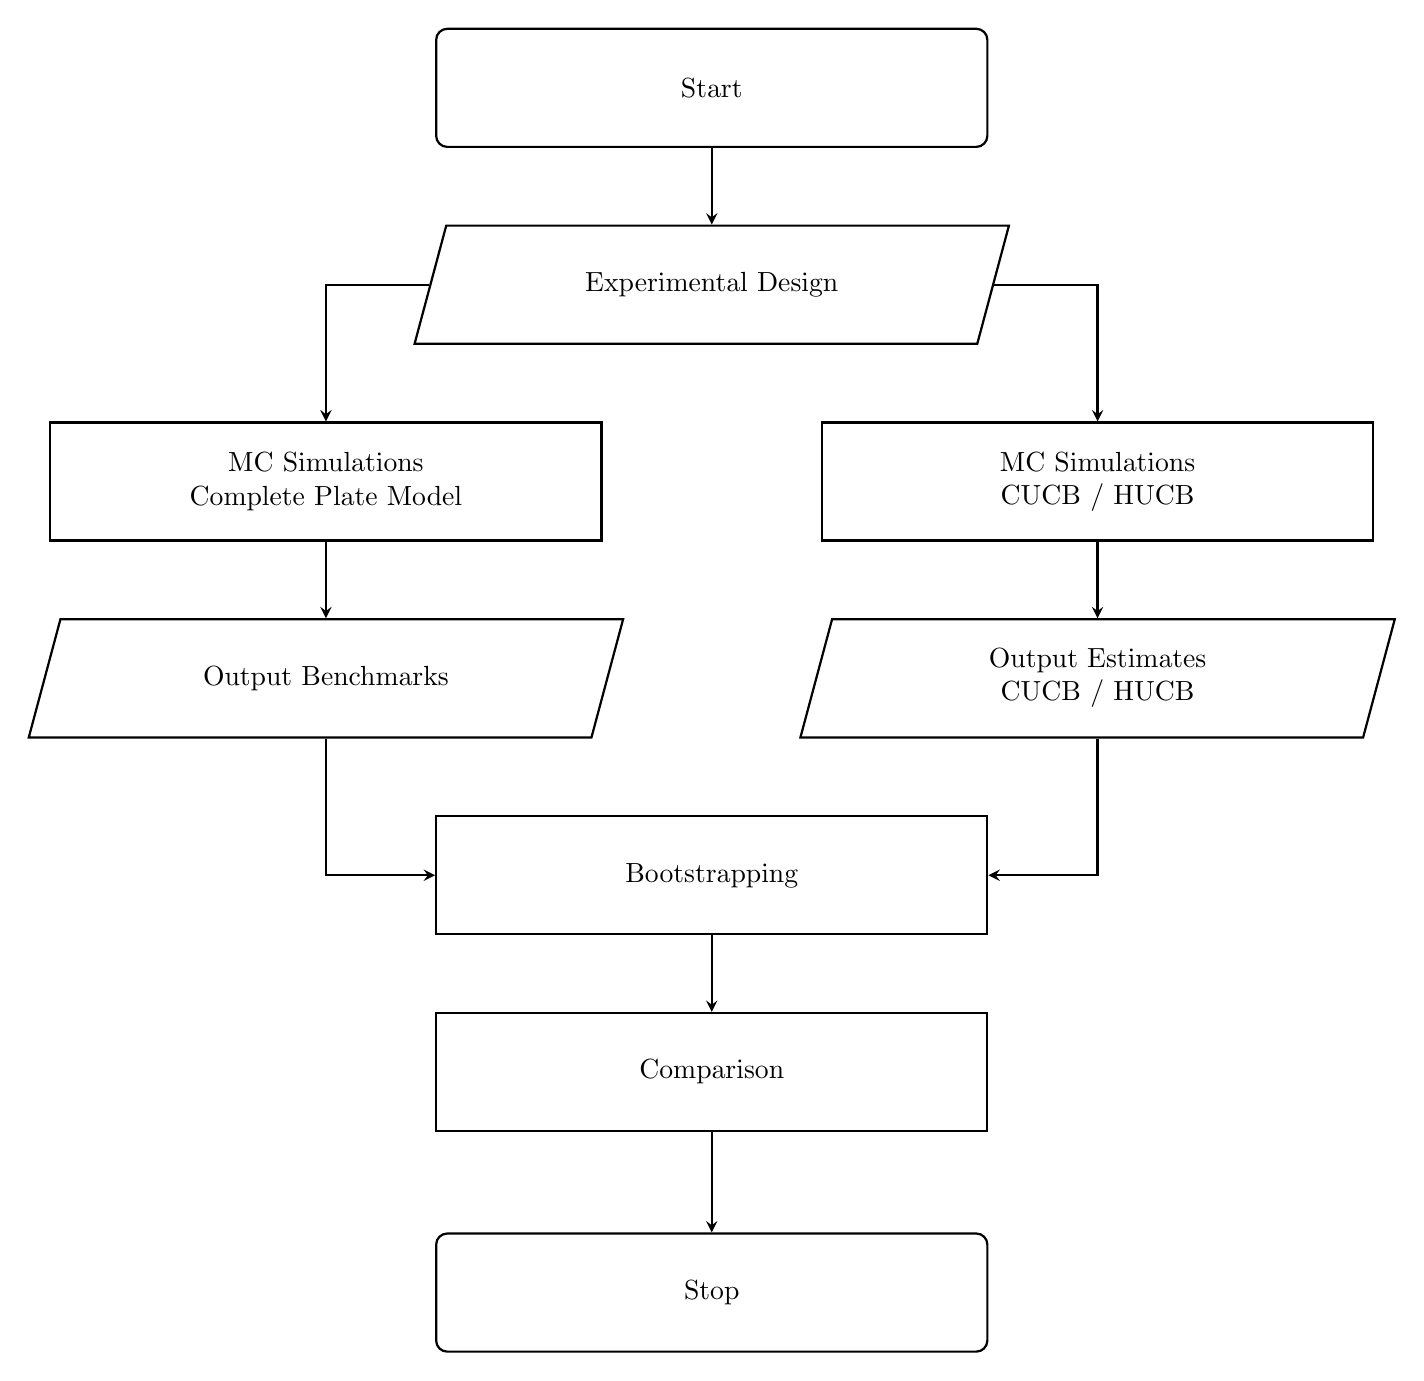
\begin{tikzpicture}[
            startstop/.style={%
                thick, rectangle, rounded corners,%
                minimum width=\charthgap, minimum height=\chartvgap,%
                text centered, draw=black, fill=white, text width=\charttwid%
            },
            io/.style={%
                thick, trapezium, trapezium left angle=75, trapezium right angle=105,%
                minimum width=\charthgap, minimum height=\chartvgap,%
                text centered, draw=black, fill=white, text width=\chartvgap%
            },
            process/.style={%
                thick, rectangle,%
                minimum width=\charthgap, minimum height=\chartvgap,%
                text centered, draw=black, fill=white, text width=\charttwid%
            },
            blankprocess/.style={%
                thick, rectangle,%
                minimum width=\charthgap, minimum height=\chartvgap,%
                text centered, draw=none, fill=none, text width=\charttwid%
            },
            decision/.style={%
                thick, diamond,%
                minimum width=\chartvgap, minimum height=\chartvgap,%
                text centered, draw=black, fill=white, text width=\chartvgap%
            },
            arrow/.style={thick,->,>=stealth}
        ]

        % Define nodes
        \node (start) [startstop] {%
            Start
        };

        \node (input1) [
                io, below of=start,
                % xshift=-0.7*\charthgap,
                yshift=-\chartvgap
            ] {$\phantom{a}$};

        \node (ED_1) [
                blankprocess, below of=start,
                % xshift=-0.7*\charthgap,
                yshift=-\chartvgap
            ] {
            Experimental Design
            };

        \node (fullEval) [
                process, below of=ED_1,
                xshift=-0.7*\charthgap,
                yshift=-\chartvgap
            ] {
                MC Simulations\\
                Complete Plate Model
            };

        \node (subEval) [
                process, below of=ED_1,
                xshift=0.7*\charthgap,
                yshift=-\chartvgap
            ] {
                MC Simulations\\
                CUCB / HUCB
            };

        \node (input5) [io, below of=subEval, yshift=-\chartvgap] {
            $\phantom{a}$
        };
        \node (ED_5) [blankprocess, below of=subEval, yshift=-\chartvgap] {
            Output Estimates\\
            CUCB / HUCB
        };

        \node (input6) [io, below of=fullEval, yshift=-\chartvgap] {
            $\phantom{a}$
        };
        \node (ED_6) [blankprocess, below of=fullEval, yshift=-\chartvgap] {
            Output Benchmarks
        };

        \path 
            (ED_5) -- (ED_6) coordinate[midway] (ED_56);

        \node (compare) [process, below of=ED_56, yshift=-\chartvgap] {
            Bootstrapping
        };
        \node (iterate) [process, below of=compare, yshift=-\chartvgap] {
            Comparison
        };
        \node (stop) [startstop, below of=iterate, yshift=-1.2*\chartvgap] {Stop};

        \draw [arrow] (start) -- (ED_1);
        \draw [arrow] (input1) -| (fullEval);
        \draw [arrow] (input1) -| (subEval);
        \draw [arrow] (fullEval) -- (ED_6);
        \draw [arrow] (subEval) -- (ED_5);
        \draw [arrow] (ED_6) |- (compare);
        \draw [arrow] (ED_5) |- (compare);
        \draw [arrow] (compare) -- (iterate);
        \draw [arrow] (iterate) -- (stop);

        % \path (start) -- (ED_1) coordinate[midway] (midpoint_1);
        % \draw [arrow] (midpoint_1) -| (ED_2);
        % \draw [arrow] (ED_2) -- (subEval);
        % \draw [arrow] (subEval) -- (ED_3);
        % \draw [arrow] (ED_3) -- (resample);
        % \draw [arrow] (resample) -- (ED_4);
        % \draw [arrow] (ED_4) -- (train);
        % \draw [arrow] (train) -- (evalRPCE);
        % \draw [arrow] (evalRPCE) -- (ED_5);
        % \draw [arrow] (ED_5) |- (compare);

        % \draw [arrow] (compare) -- (iterate);
        % \draw [arrow] (iterate) -- node[right] {n} (stop) ;

        % \draw [thick] 
        %     (iterate) -- 
        %     ++(1.2*\chartvgap,0) node[midway, above] {y} coordinate (endpoint_1);
        % \draw [thick] 
        %     (endpoint_1) -- node[above] {$i=i+1$}
        %     ++(1.0*\charthgap,0) coordinate (endpoint_2);

        % \draw [arrow] 
        %     (endpoint_2) |- (resample);

        % \path 
        %     (ED_1) -- (fullEval) coordinate[midway] (point_1);
        % \path 
        %     (ED_2) -- (subEval) coordinate[midway] (point_2);
        % \path 
        %     (point_1) -- (point_2) coordinate[midway] (point_3);
        % \draw [thick] 
        %     (point_1) -- (point_3);
        % \draw [arrow] 
        %     (point_3) |- (evalRPCE);

        \end{tikzpicture}
    }
    \caption{The UCBs Evaluation Procedure Flowchart}
    \label{flowchart: UCB procedure}
\end{figure}

Subsequently, the author evaluates the performance of HUCB + NI-RPCE models in approximating the complete plate model.
The author generates two EDs of size $N_{ed}=300$ through random sampling.
The first ED is for direct MCS using the complete plate model.
Similar to the procedure above, the outputs serve as the benchmark for comparison.
Then, the author runs MCS for FRFs using the substructured plate model with the HUCB methods, using the second ED.
The outputs serve as the pool of training data for the RPCE models.
The training process of the RPCE models follows, using a random subset of these training data.
The author then feeds the first ED to the trained model.
Afterward, the comparisons between the outputs with the benchmark and error calculations follow.
To take into account the effect of the training data, the author varies the size of the random subset and repeats these steps $N=40$ times for each subset's size.
Figure \ref{flowchart: framework procedure} illustrates the evaluation procedure.
% -----------------------------------------------------------------------------
% Master thesis in the study program computational mechanics
%
% B.Sc. Rezha Adrian Tanuharja - 03751261
% M.Sc. Felix Schneider (supervisor)
%
% images/procedureFramework.tex
% Last edited 03 November 2023
% -----------------------------------------------------------------------------

\begin{figure}[H]
    \centering
    \scalebox{0.75}{
        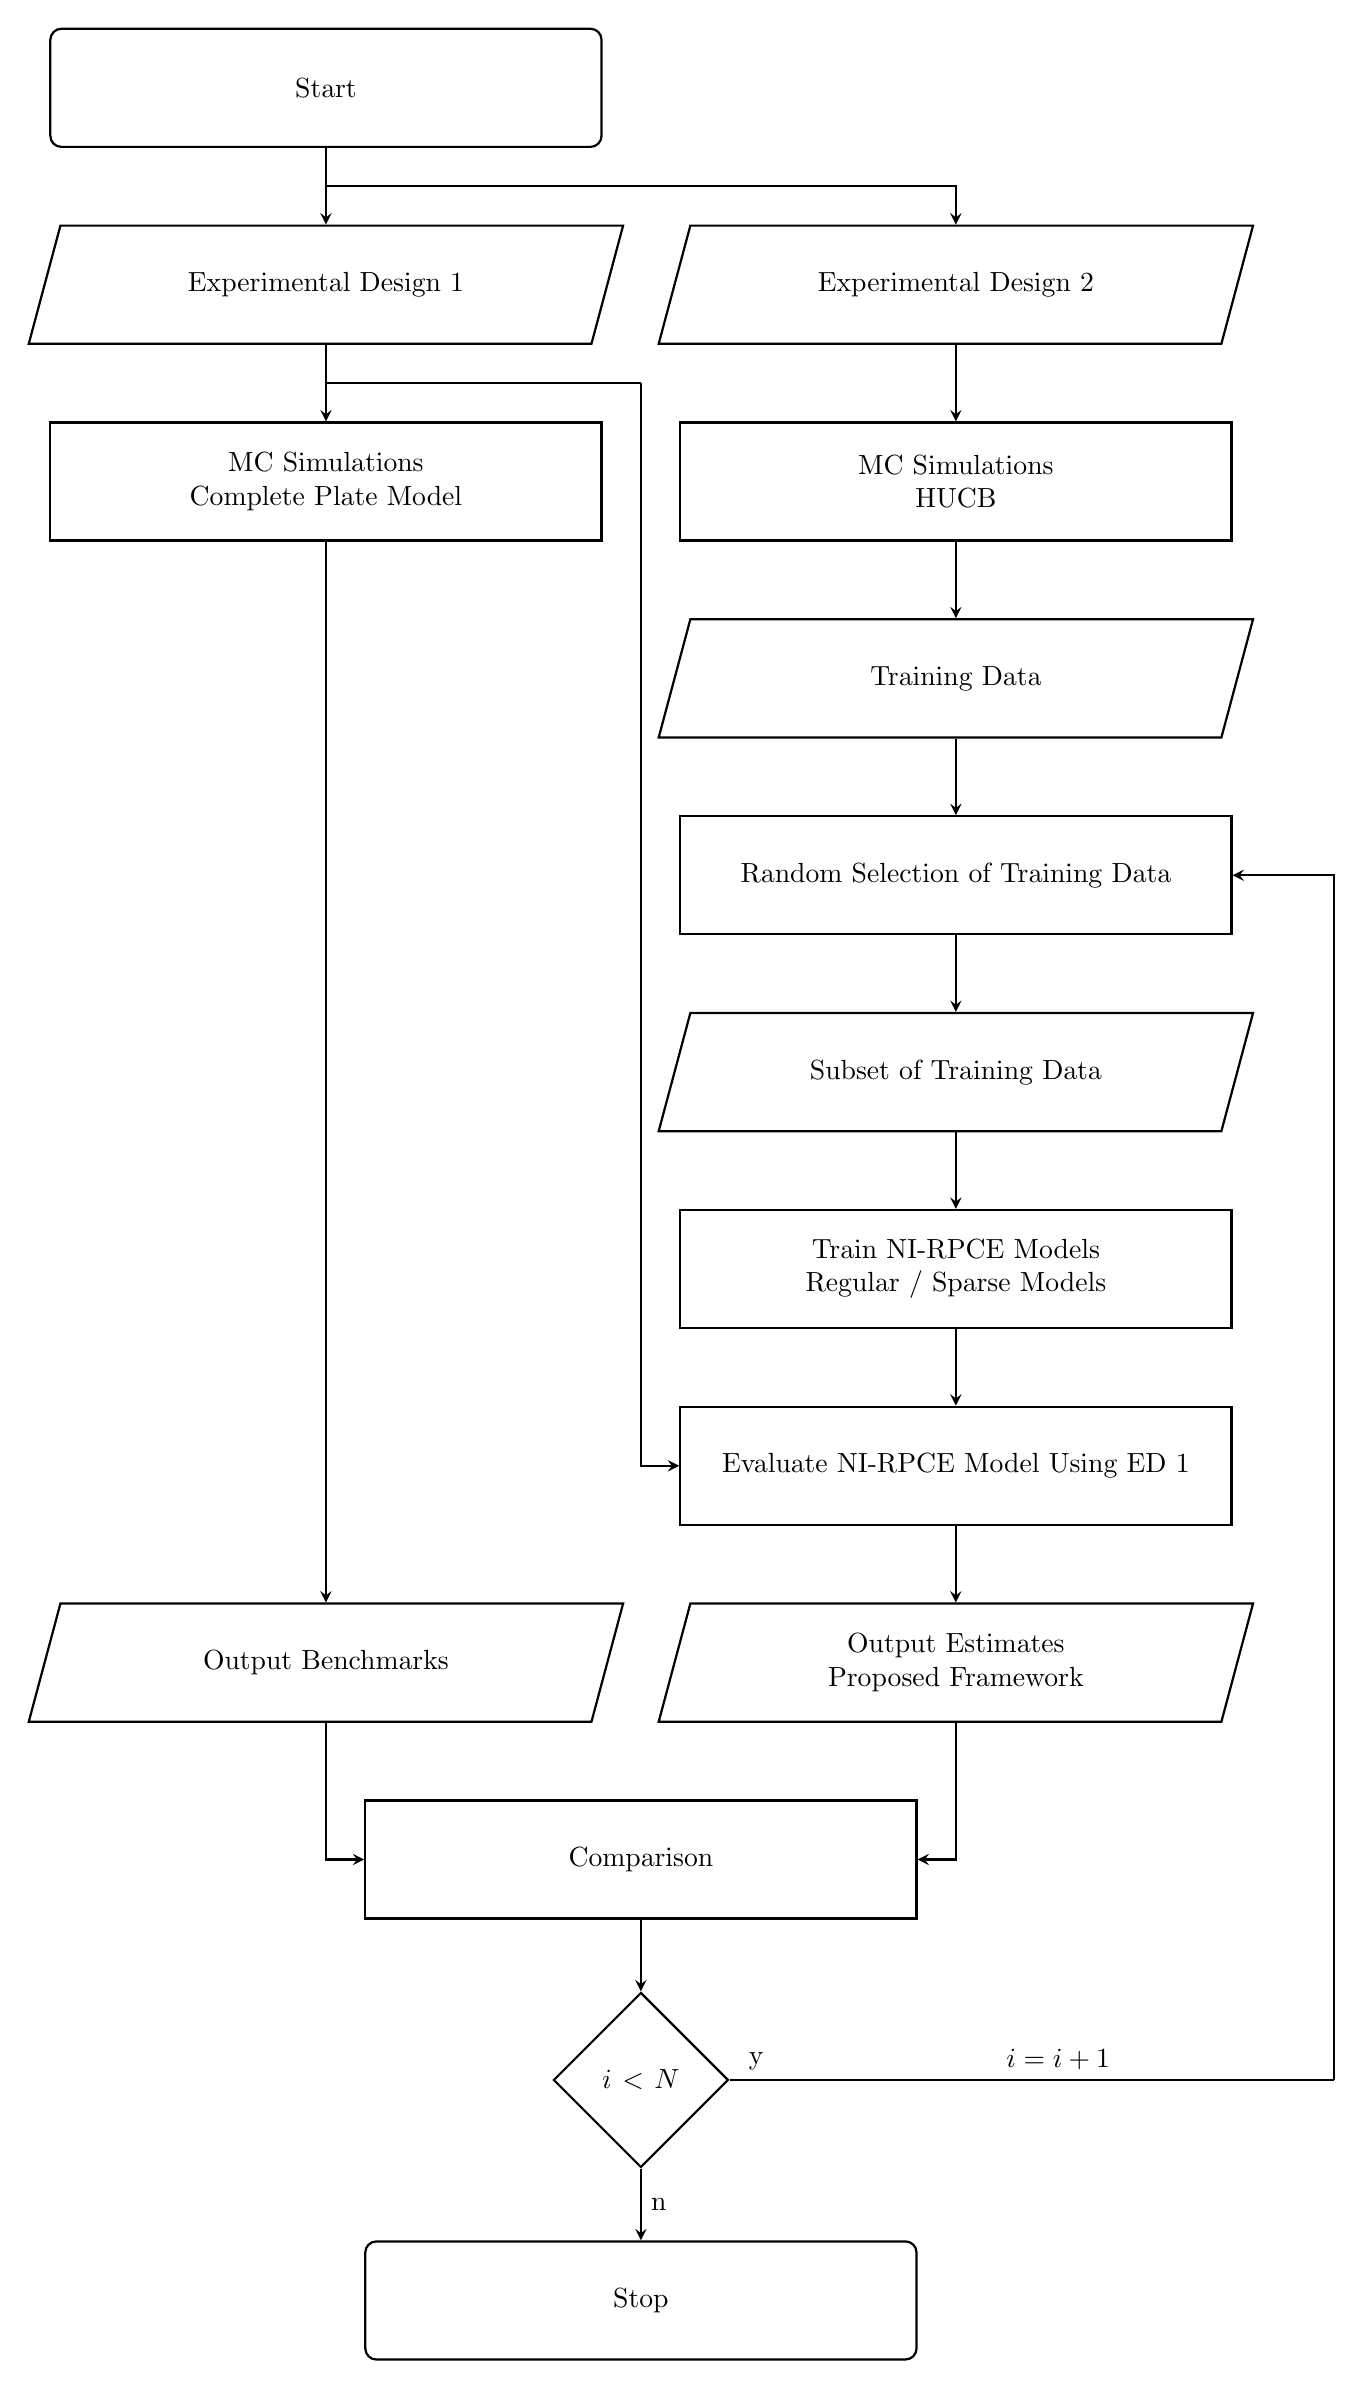
\begin{tikzpicture}[
            startstop/.style={%
                thick, rectangle, rounded corners,%
                minimum width=\charthgap, minimum height=\chartvgap,%
                text centered, draw=black, fill=white, text width=\charttwid%
            },
            io/.style={%
                thick, trapezium, trapezium left angle=75, trapezium right angle=105,%
                minimum width=\charthgap, minimum height=\chartvgap,%
                text centered, draw=black, fill=white, text width=\chartvgap%
            },
            process/.style={%
                thick, rectangle,%
                minimum width=\charthgap, minimum height=\chartvgap,%
                text centered, draw=black, fill=white, text width=\charttwid%
            },
            blankprocess/.style={%
                thick, rectangle,%
                minimum width=\charthgap, minimum height=\chartvgap,%
                text centered, draw=none, fill=none, text width=\charttwid%
            },
            decision/.style={%
                thick, diamond,%
                minimum width=\chartvgap, minimum height=\chartvgap,%
                text centered, draw=black, fill=white, text width=\chartvgap%
            },
            arrow/.style={thick,->,>=stealth}
        ]

        % Define nodes
        \node (start) [startstop] {%
            Start
        };
        \node (input1) [io, below of=start, yshift=-\chartvgap] {$\phantom{a}$};
        \node (ED_1) [blankprocess, below of=start, yshift=-\chartvgap] {
            Experimental Design 1
            % $\left\{\mathbf{X}_{1}, ..., \mathbf{X}_{n}\right\}$
        };
        \node (fullEval) [process, below of=ED_1, yshift=-\chartvgap] {
            MC Simulations\\
            Complete Plate Model
        };
        \node (input2) [io, right of=ED_1, xshift=\charthgap] {$\phantom{a}$};
        \node (ED_2) [blankprocess, right of=ED_1, xshift=\charthgap] {
            Experimental Design 2
            % $\left\{\widetilde{\mathbf{X}}_{1}, ..., 
            % \widetilde{\mathbf{X}}_{n}\right\}$
        };
        \node (subEval) [process, below of=ED_2, yshift=-\chartvgap] {
            MC Simulations\\
            HUCB 
        };
        \node (input3) [io, below of=subEval, yshift=-\chartvgap] {
            $\phantom{a}$
        };
        \node (ED_3) [blankprocess, below of=subEval, yshift=-\chartvgap] {
            Training Data
            % $\widetilde{\mathcal{M}}\left(
            %     \widetilde{\mathbf{X}}_{1}
            % \right), ...,
            % \widetilde{\mathcal{M}}\left(
            %     \widetilde{\mathbf{X}}_{n}
            % \right)$
        };
        \node (resample) [process, below of=ED_3, yshift=-\chartvgap] {
            Random Selection of Training Data
        };
        \node (input4) [io, below of=resample, yshift=-\chartvgap] {
            $\phantom{a}$
        };
        \node (ED_4) [blankprocess, below of=resample, yshift=-\chartvgap] {
            Subset of Training Data
        };
        \node (train) [process, below of=ED_4, yshift=-\chartvgap] {
            Train NI-RPCE Models\\
            Regular / Sparse Models
        };
        \node (evalRPCE) [process, below of=train, yshift=-\chartvgap] {
            Evaluate NI-RPCE Model Using ED 1
        };
        \node (input5) [io, below of=evalRPCE, yshift=-\chartvgap] {
            $\phantom{a}$
        };
        \node (ED_5) [blankprocess, below of=evalRPCE, yshift=-\chartvgap] {
            Output Estimates\\
            Proposed Framework
        };
        \node (input6) [io, left of=ED_5, xshift=-\charthgap] {
            $\phantom{a}$
        };
        \node (ED_6) [blankprocess, left of=ED_5, xshift=-\charthgap] {
            Output Benchmarks
        };

        \path 
            (ED_5) -- (ED_6) coordinate[midway] (ED_56);

        \node (compare) [process, below of=ED_56, yshift=-\chartvgap] {
            Comparison
        };
        \node (iterate) [decision, below of=compare, yshift=-1.2*\chartvgap] {
            $i < N$
        };
        \node (stop) [startstop, below of=iterate, yshift=-1.2*\chartvgap] {Stop};

        \draw [arrow] (start) -- (ED_1);
        \draw [arrow] (ED_1) -- (fullEval);
        \draw [arrow] (fullEval) -- (ED_6);
        \draw [arrow] (ED_6) |- (compare);

        \path (start) -- (ED_1) coordinate[midway] (midpoint_1);
        \draw [arrow] (midpoint_1) -| (ED_2);
        \draw [arrow] (ED_2) -- (subEval);
        \draw [arrow] (subEval) -- (ED_3);
        \draw [arrow] (ED_3) -- (resample);
        \draw [arrow] (resample) -- (ED_4);
        \draw [arrow] (ED_4) -- (train);
        \draw [arrow] (train) -- (evalRPCE);
        \draw [arrow] (evalRPCE) -- (ED_5);
        \draw [arrow] (ED_5) |- (compare);

        \draw [arrow] (compare) -- (iterate);
        \draw [arrow] (iterate) -- node[right] {n} (stop) ;

        \draw [thick] 
            (iterate) -- 
            ++(1.2*\chartvgap,0) node[midway, above] {y} coordinate (endpoint_1);
        \draw [thick] 
            (endpoint_1) -- node[above] {$i=i+1$}
            ++(1.0*\charthgap,0) coordinate (endpoint_2);

        \draw [arrow] 
            (endpoint_2) |- (resample);

        \path 
            (ED_1) -- (fullEval) coordinate[midway] (point_1);
        \path 
            (ED_2) -- (subEval) coordinate[midway] (point_2);
        \path 
            (point_1) -- (point_2) coordinate[midway] (point_3);
        \draw [thick] 
            (point_1) -- (point_3);
        \draw [arrow] 
            (point_3) |- (evalRPCE);

        \end{tikzpicture}
    }
    \caption{The Proposed Framework Evaluation Procedure Flowchart}
    \label{flowchart: framework procedure}
\end{figure}
% -----------------------------------------------------------------------------
% Master thesis in the study program computational mechanics
%
% B.Sc. Rezha Adrian Tanuharja - 03751261
% M.Sc. Felix Schneider (supervisor)
%
% chapters/methodology/measure.tex
% Last edited 03 November 2023
% -----------------------------------------------------------------------------

\section{Error Measure}
\label{sec: performance measure}

This study compares the proposed framework's outputs against the outputs of direct MCS.
Two kinds of error measures quantify the framework's performance: relative empirical error and response statistic relative error.

\subsection{Relative Empirical Error}
\label{ssec: pointwise error}

This error measure quantifies the difference in the outputs of two models when using the same set of input parameters.
For the complete plate model $\mathcal{M}$, the RPCE model $\widehat{\mathcal{M}}$ and the size of the first experimental design $N_{ed}$, the empirical error is:
\begin{equation}
    err_{emp} \left(\omega\right)
    =
    \frac{1}{N_{ed}} \sum_{i=1}^{N_{ed}}{
        \left|
            \widehat{\mathcal{M}} \left(
                \omega, \mathbf{\Xi}_{i}
            \right)
            -
            \mathcal{M} \left(
                \omega, \mathbf{\Xi}_{i}
            \right)
        \right|^{2}
    }.
\end{equation}
The relative empirical error is the ratio between the empirical error and the sample variance of the outputs from direct MC simulations:
\begin{equation}
    \epsilon_{emp} \left(\omega\right)
    =
    \frac{
        err_{emp} \left(\omega\right)
    }{
        \widehat{\text{Var}}\left(
            \mathcal{M}\left(
                \omega, \mathbf{\Xi}
            \right)
        \right)
    }.
\end{equation}

\subsection{Response Statistic Relative Error}
\label{ssec: statistic error}

This error measure quantifies the difference in the outputs' statistics of two models when being fed the same ED.
For an outputs' statistic of the complete plate model $m\left(\omega\right)$ and the outputs' statistic of the proposed framework $\widehat{m}\left(\omega\right)$, the relative error is:
\begin{equation}
    \epsilon_{rel, m} \left(\omega\right)
    =
    \frac{
        \left|
            \widehat{m}\left(\omega\right)
            -
            m\left(\omega\right)
        \right|
    }{
        \left|
            m\left(\omega\right)
        \right|
    }
\end{equation}
The outputs' statistics of interest in this study are the means and variances of the outputs.
% -----------------------------------------------------------------------------
% Master thesis in the study program computational mechanics
%
% B.Sc. Rezha Adrian Tanuharja - 03751261
% M.Sc. Felix Schneider (supervisor)
%
% chapters/discussion.tex
% Last edited 03 November 2023
% -----------------------------------------------------------------------------

\chapter{Findings and Discussion}
\label{ch: discussion}

% -----------------------------------------------------------------------------
% Master thesis in the study program computational mechanics
%
% B.Sc. Rezha Adrian Tanuharja - 03751261
% M.Sc. Felix Schneider (supervisor)
%
% chapters/discussion/substructuring.tex
% Last edited 03 November 2023
% -----------------------------------------------------------------------------

\section{Dynamic Substructuring}
\label{sec: performance of cms}

This section reports the findings from the first half of the proposed framework: dynamic substructuring for models with parametric uncertainties. 
These findings come from observing the plate's vertical acceleration at nodes A and B when subjected to a unit vertical force at node A.
Details about the nodes are available in chapter \ref{ch: methodology}.

% -----------------------------------------------------------------------------
% Master thesis in the study program computational mechanics
%
% B.Sc. Rezha Adrian Tanuharja - 03751261
% M.Sc. Felix Schneider (supervisor)
%
% chapters/discussion/substructuring/point_A.tex
% Last edited 03 November 2023
% -----------------------------------------------------------------------------

\subsection{Vertical Acceleration at Node A}
\label{ssec: cms point A}

Figure \ref{FRF_MC_A_A_linear} shows the FRFs from direct MCS of the complete plate model.
These FRFs relate the vertical acceleration magnitude at point A to a unit force at the same point at discrete frequencies in the range $\left[9.0, 17.5\right]$ rad/s with increments of $0.5$ rad/s.
The outliers are intentionally missing to enable a clear view of the FRFs' statistics: their medians, interquartile ranges, and whiskers.
\begin{figure}[H]
    \centering
    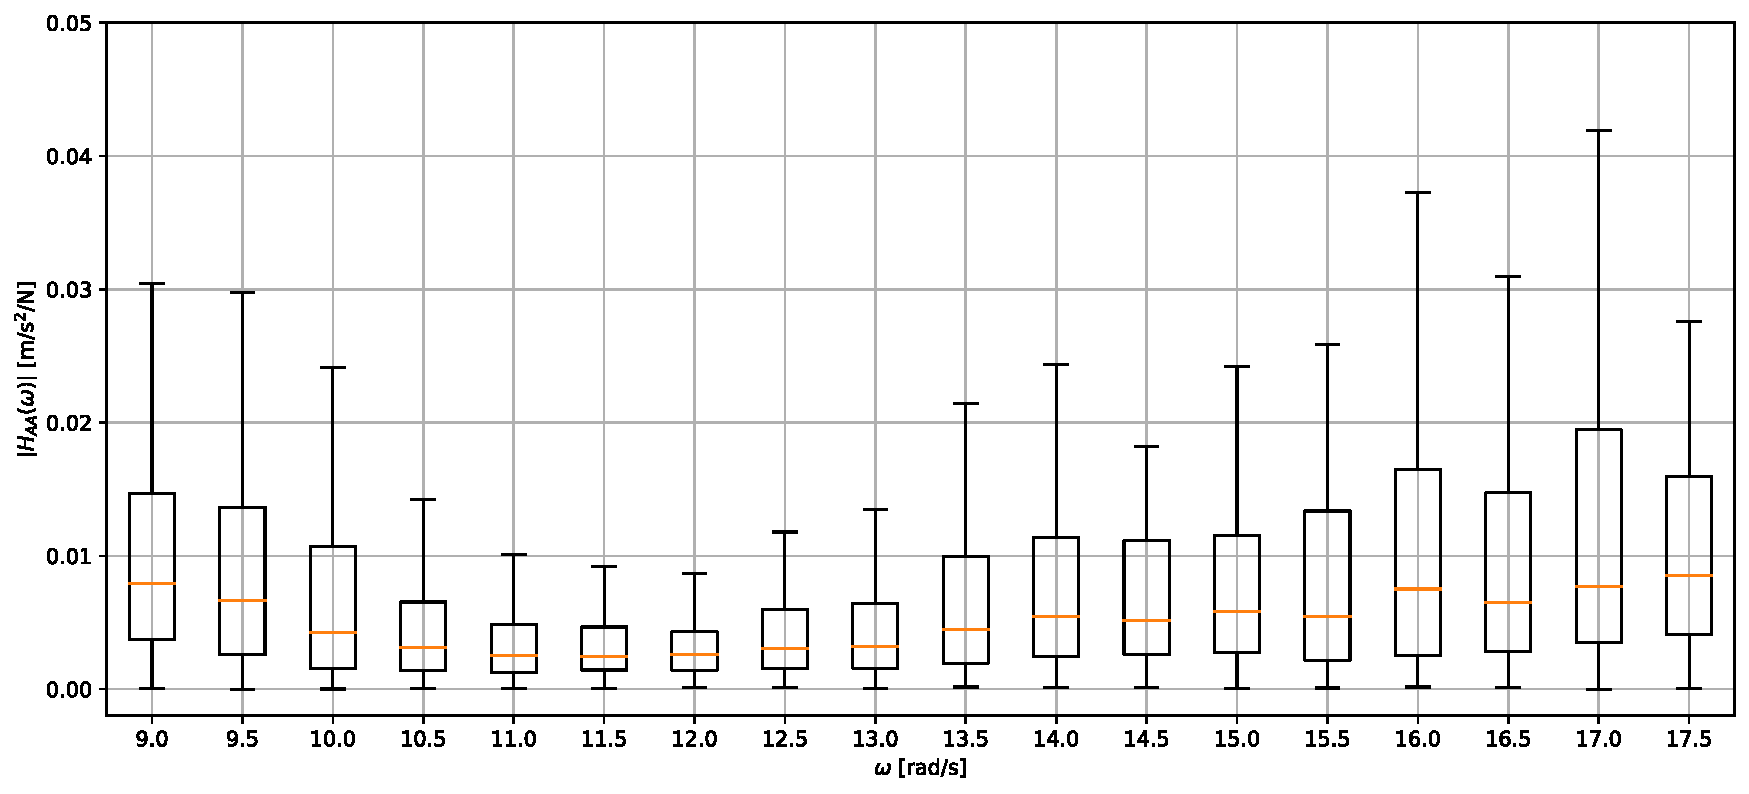
\includegraphics[width=1.0\textwidth]{
        plots/substructuring/plot_1_linear.pdf
    }
    \caption{%
        $\left|H_{AA}\right|$ from Direct MCS of The Complete Plate Model
    }
    \label{FRF_MC_A_A_linear}
\end{figure}
Figure \ref{FRF_MC_A_A_log} shows the same FRFs as figure \ref{FRF_MC_A_A_linear} with outliers.
The logarithmic scale provides a clear view of the outliers and the low whiskers of the plot.
The figure shows that the outlier values can be larger by approximately two orders of magnitudes compared to the medians.
\begin{figure}[H]
    \centering
    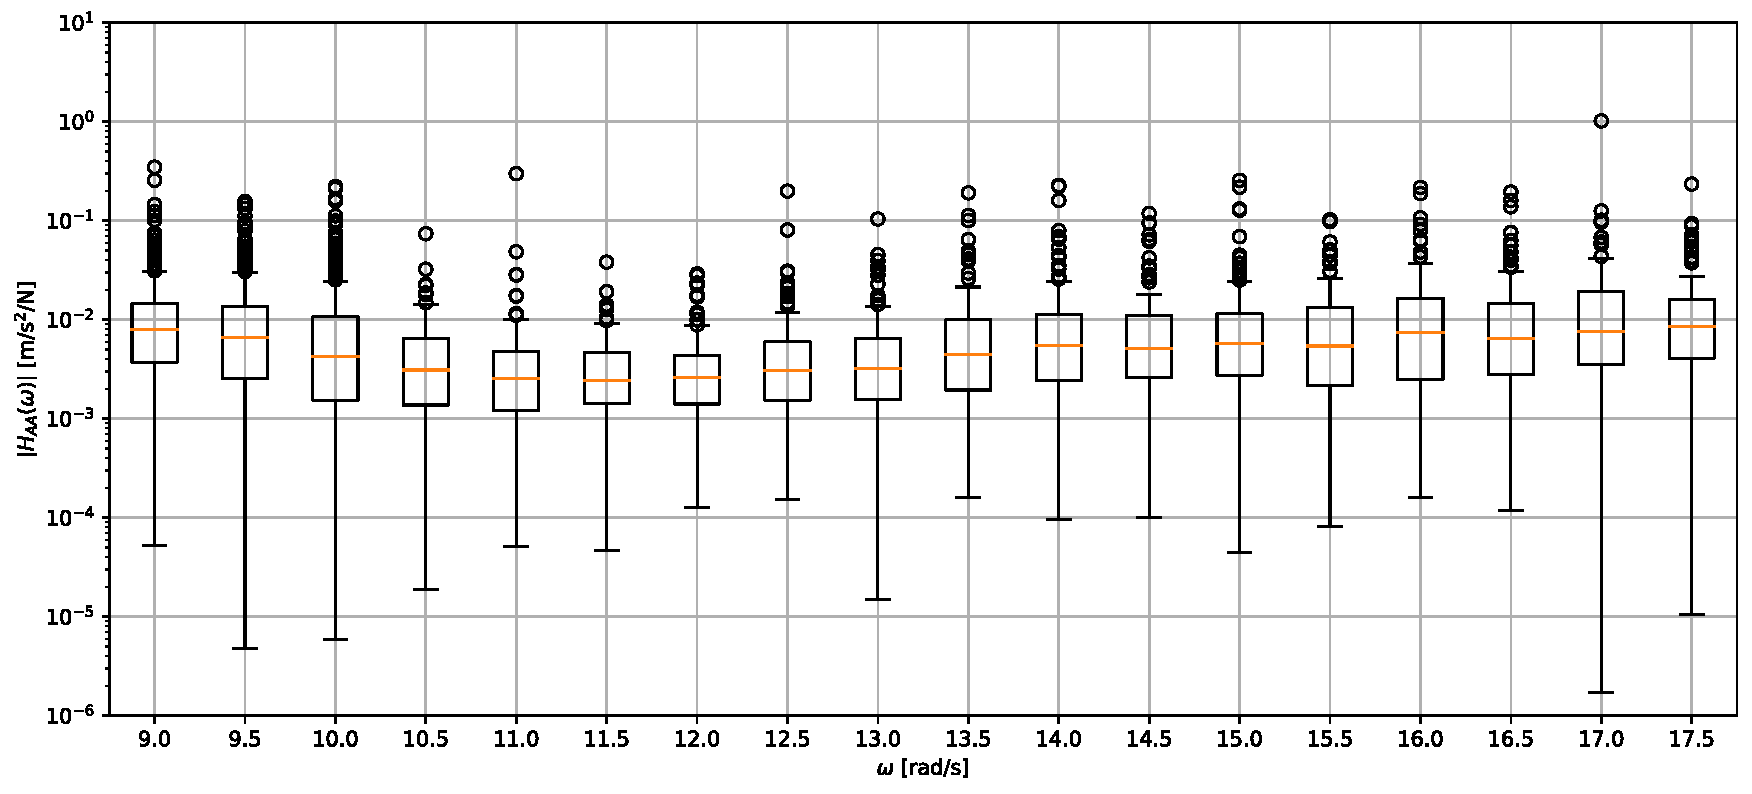
\includegraphics[width=1.0\textwidth]{
        plots/substructuring/plot_1_log.pdf
    }
    \caption{%
        $\left|H_{AA}\right|$ from Direct MCS of The Complete Plate Model with Outliers
    }
    \label{FRF_MC_A_A_log}
\end{figure}
First, the author analyzes the performance of the CUCB method.
Figure \ref{e_emp CUCB_A_A} shows the median relative empirical errors for the method in each frequency in the above range using three different numbers of internal modes.
The medians come from the bootstrapping method with a $1000$ number of resamplings.
\begin{figure}[H]
    \centering
    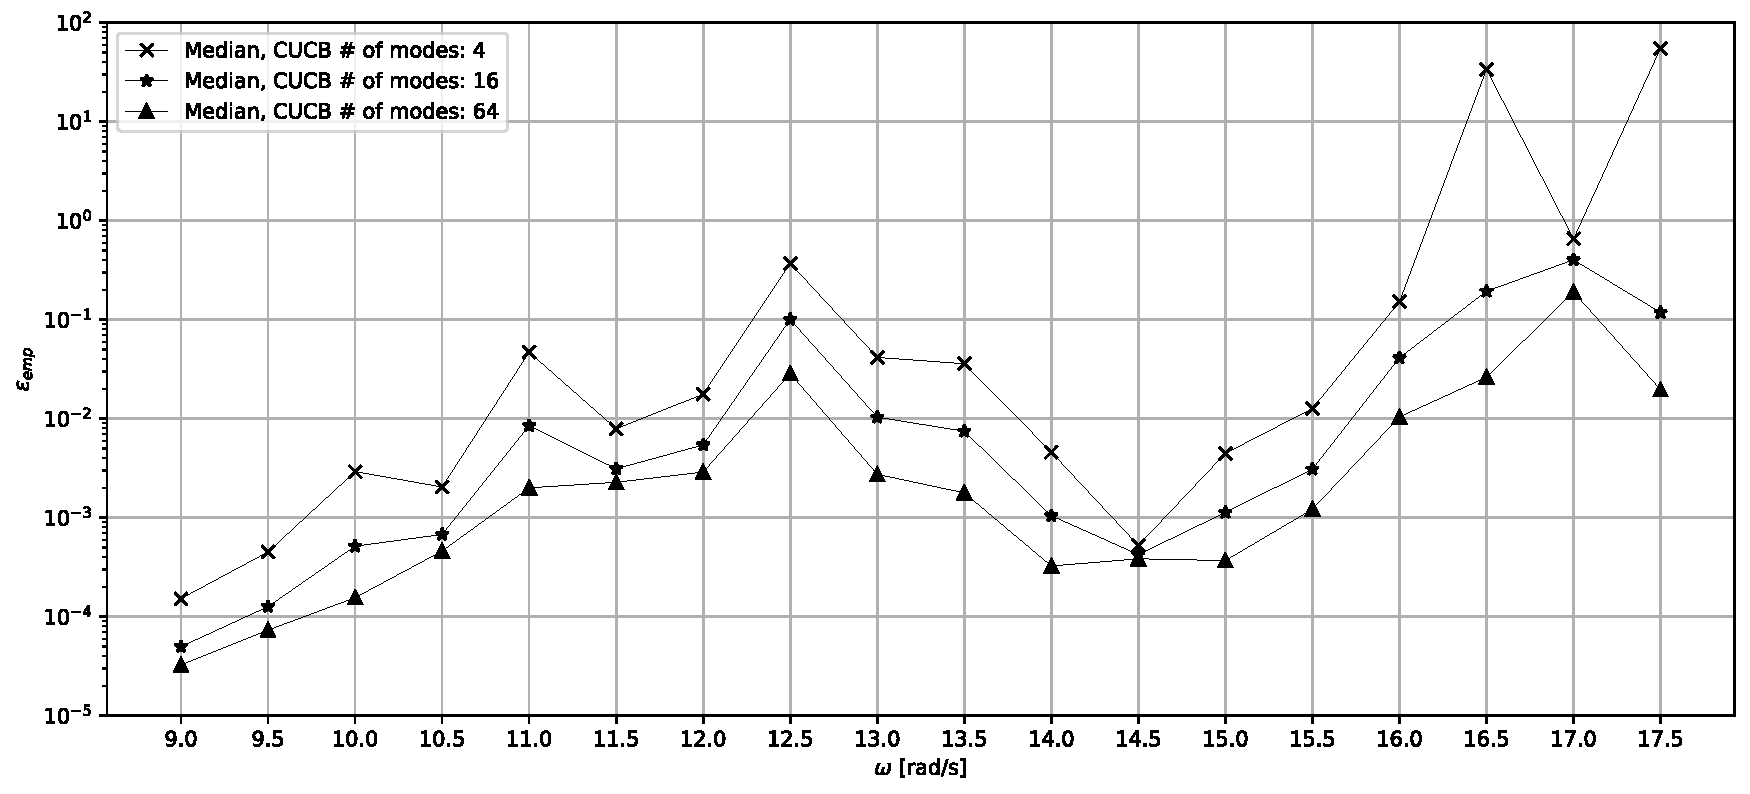
\includegraphics[width=1.0\textwidth]{
        plots/substructuring/plot_2.pdf
    }
    \caption{%
        Relative Empirical Errors of $H_{AA}$ for The CUCB Method
    }
    \label{e_emp CUCB_A_A}
\end{figure}
In deterministic dynamic substructuring, errors decrease as the number of internal modes increases.
When all internal modes are present in the model, the assembled components are equivalent to the complete structure in a mathematical sense.
Figure \ref{e_emp CUCB_A_A} exhibits the same trend for dynamic structuring using the CUCB method: as the number of internal modes increases, the relative empirical errors decrease.
However, the relative empirical errors exceeds $10^{-1}$ at $\omega=17.0$ rad/s even when using $64$ internal modes.
Therefore, the mean square errors are in the same order of magnitude as the FRFs' variance at this frequency.

Subsequently, the author analyzes the performance of the HUCB method.
Figure \ref{e_emp HUCB_A_A} shows the medians and $95\%$ confidence intervals of the relative empirical errors for the crude and hybrid UCB methods.
Figure \ref{e_emp HUCB_A_A} shows that the relative empirical errors from the HUCB method do not exceed $10^{-2}$ in this example and in most frequencies in the range lie below $10^{-3}$.
The computational cost of the HUCB method is higher than that of the CUCB method because of the evaluation of the boundary modes for each input parameter's realization.
However, it leads to lower overall relative empirical errors and, in some frequencies, reduces the errors by up to two orders of magnitudes.
\begin{figure}[H]
    \centering
    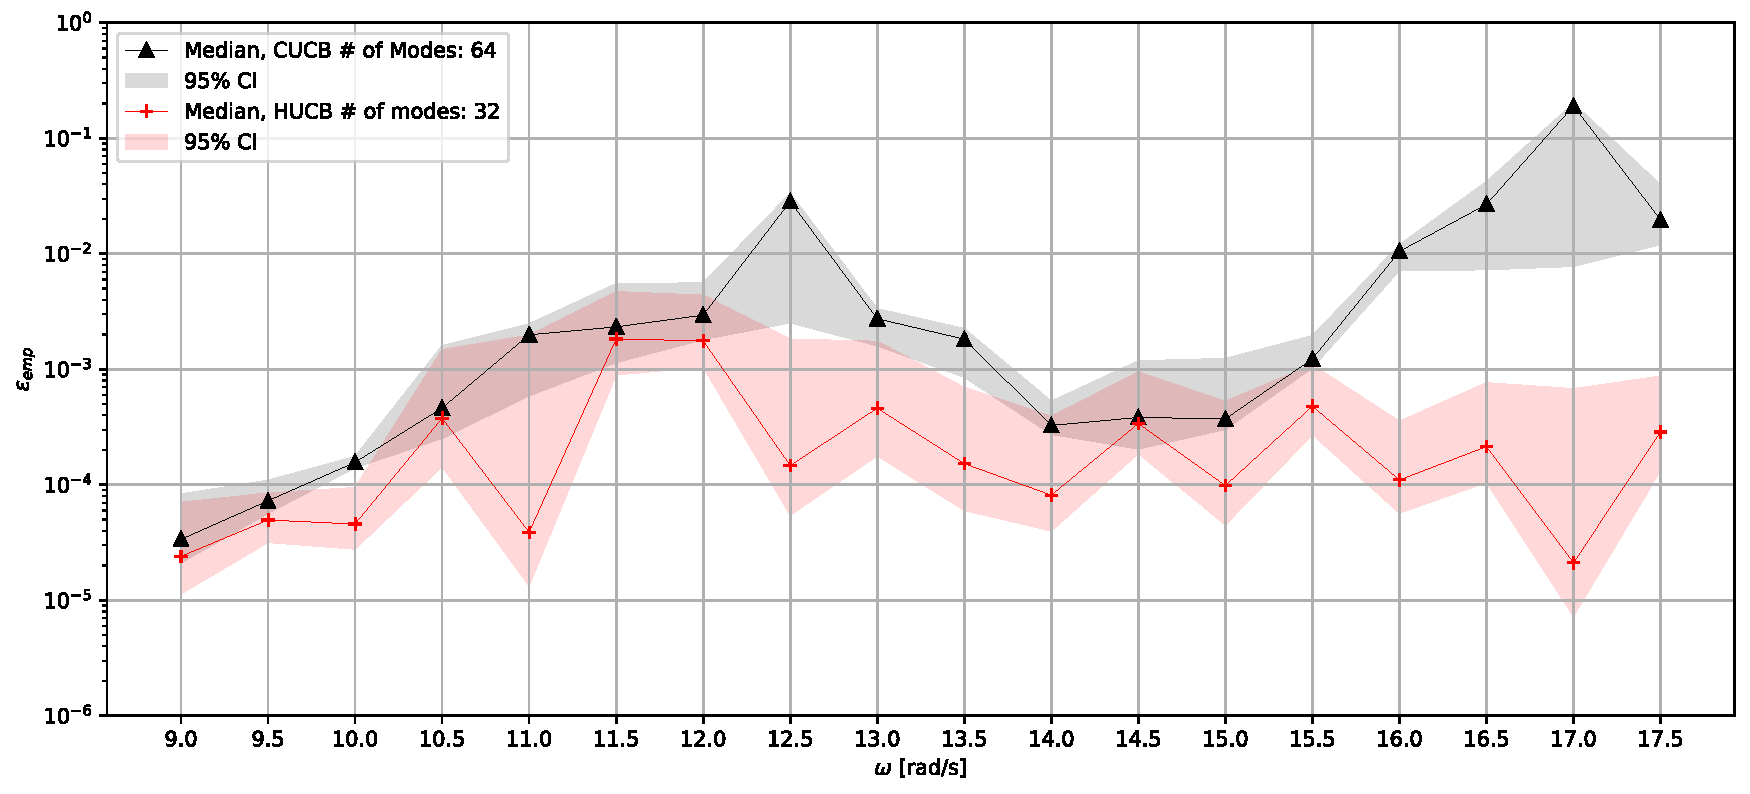
\includegraphics[width=1.0\textwidth]{
        plots/substructuring/plot_3.pdf
    }
    \caption{%
        Relative Empirical Errors of $H_{AA}$ for The CUCB and HUCB Methods
    }
    \label{e_emp HUCB_A_A}
\end{figure}

To dive deeper into the difference between the crude and hybrid UCB methods, the author evaluates the relative mean and variance errors.
Figure \ref{e_mean CUCB_A_A} shows the median relative mean errors of the FRFs' magnitudes for the CUCB method using three different numbers of internal modes.
\begin{figure}[H]
    \centering
    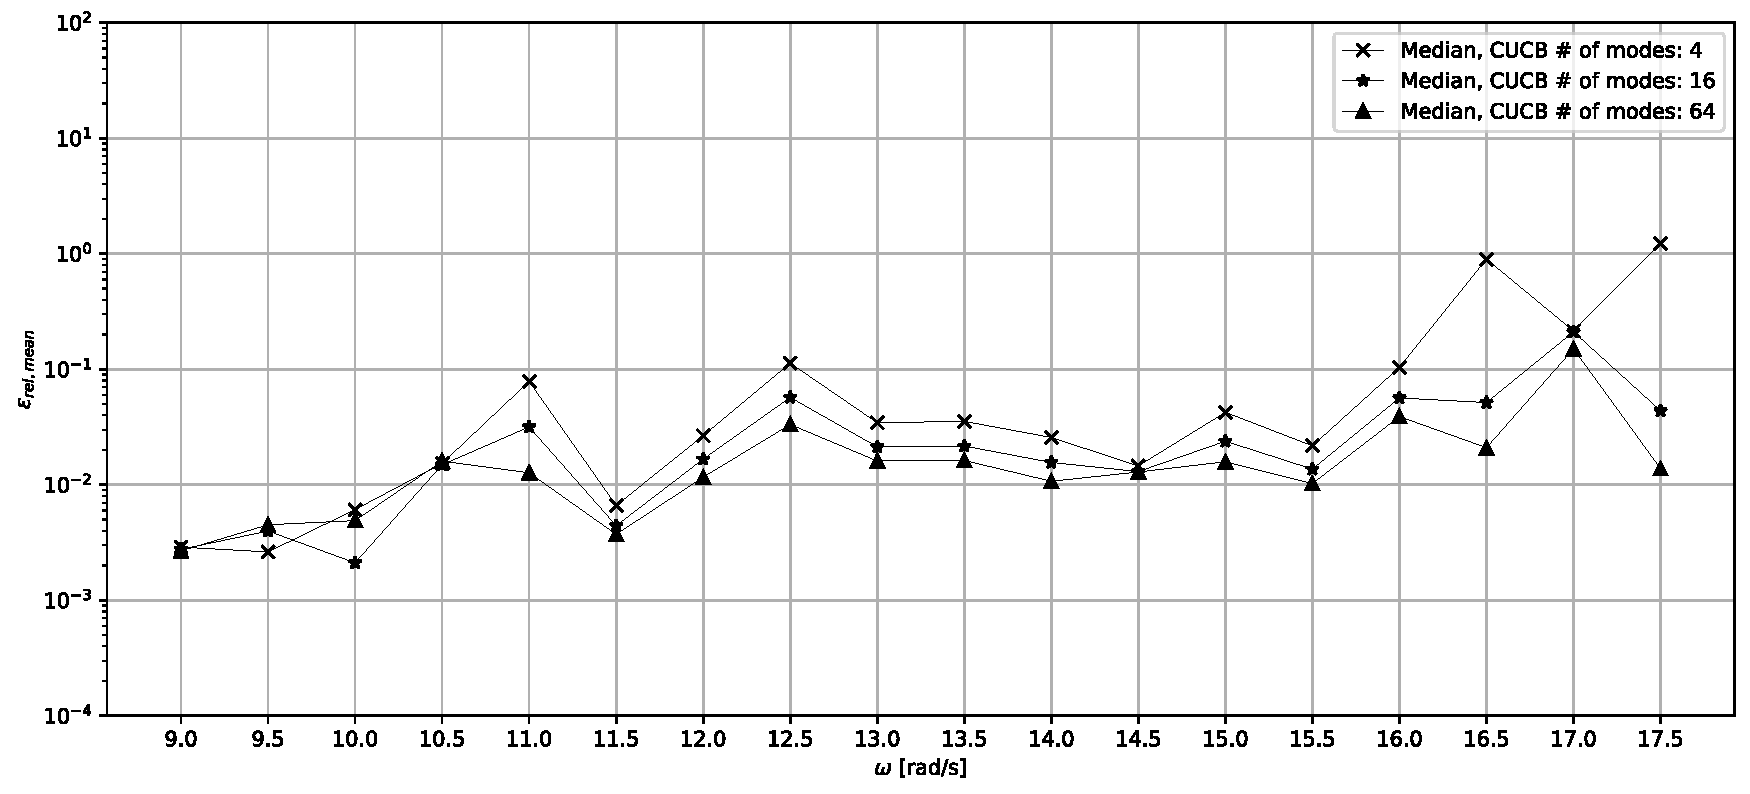
\includegraphics[width=1.0\textwidth]{
        plots/substructuring/plot_4.pdf
    }
    \caption{%
        Relative Mean Errors of $\left|H_{AA}\right|$ for The CUCB Method
    }
    \label{e_mean CUCB_A_A}
\end{figure}
Figure \ref{e_var CUCB_A_A} shows the median relative variance errors of the FRFs for the CUCB method using three different numbers of internal modes.
\begin{figure}[H]
    \centering
    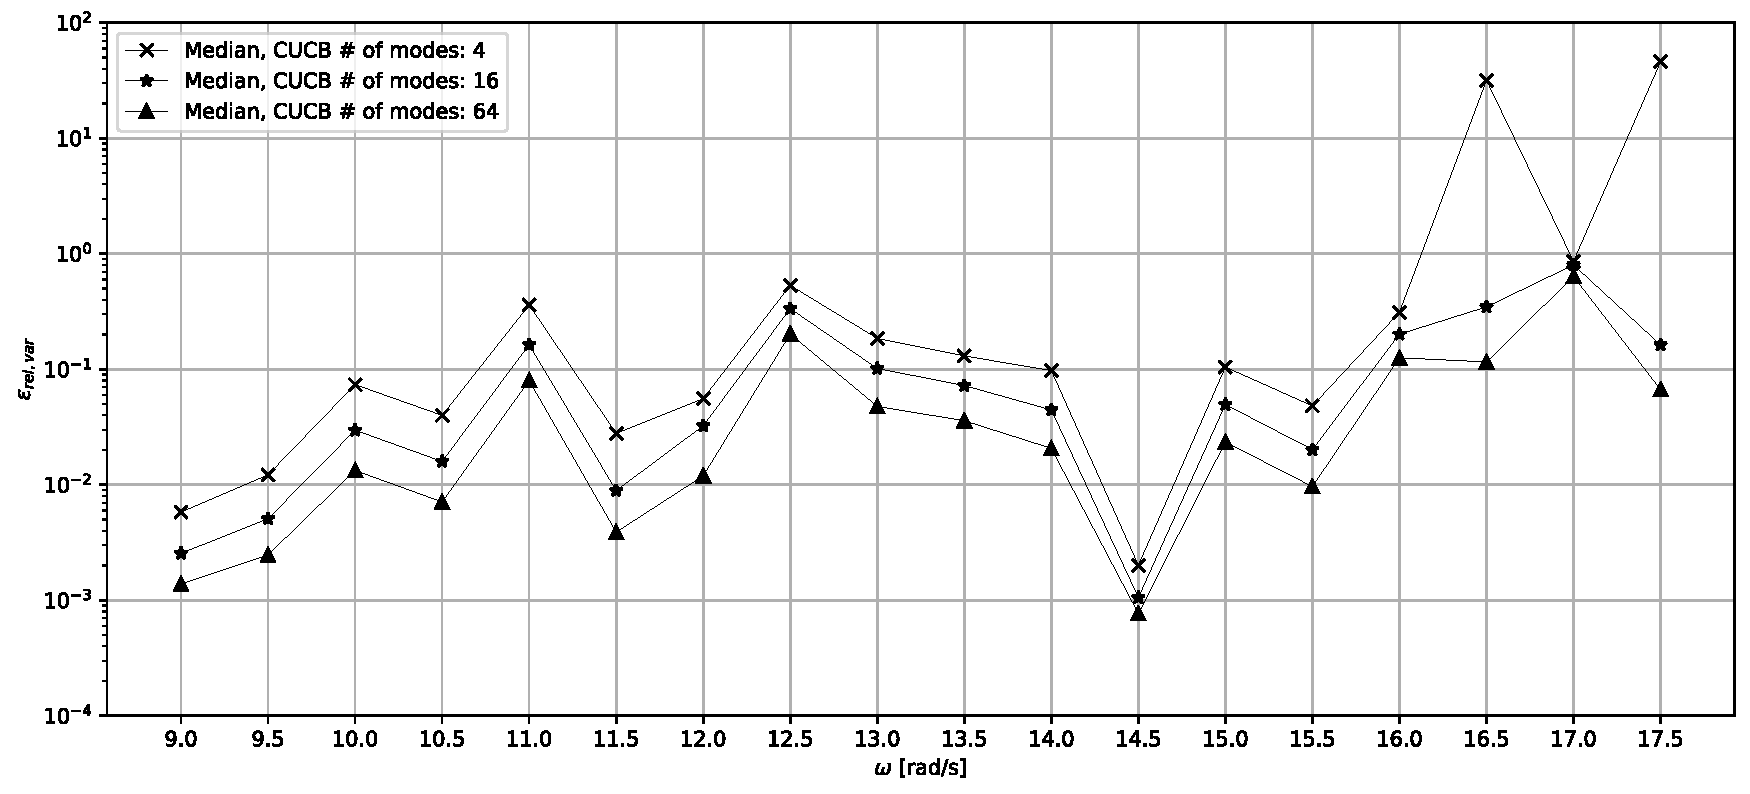
\includegraphics[width=1.0\textwidth]{
        plots/substructuring/plot_5.pdf
    }
    \caption{%
        Relative Variance Errors of $H_{AA}$ for The CUCB Method
    }
    \label{e_var CUCB_A_A}
\end{figure}
The two figures above exhibit similar trends with figure \ref{e_emp CUCB_A_A}: the relative mean errors decrease as the number of internal modes increases, with an exception at $\omega=9.5$ rad/s for the relative mean errors.
Overall, the relative mean errors and relative variance errors primarily lie between $10^{-3}$ and $10^{0}$.

Subsequently, the author compares the relative mean errors and relative variance errors for the CUCB method and the HUCB method.
Figure \ref{e_mean HUCB_A_A} shows the medians and $95\%$ confidence intervals of the relative mean errors of the FRFs' magnitudes in each frequency in the above range for the crude and hybrid UCB methods.
\begin{figure}[H]
    \centering
    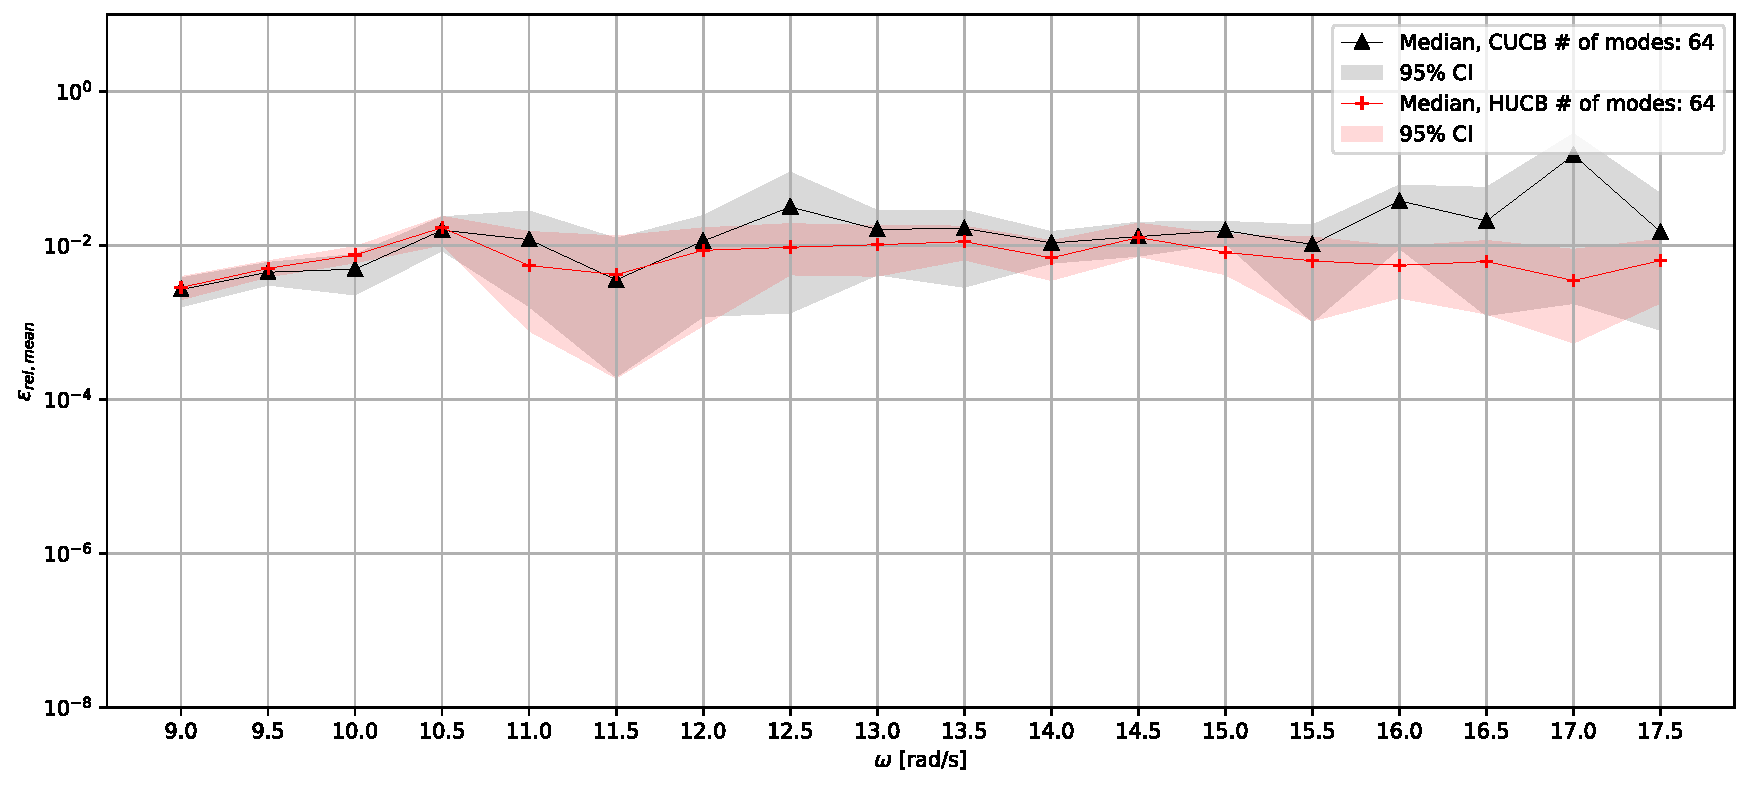
\includegraphics[width=1.0\textwidth]{
        plots/substructuring/plot_6.pdf
    }
    \caption{%
        Relative Mean Errors of $\left|H_{AA}\right|$ for The CUCB and HUCB Methods
    }
    \label{e_mean HUCB_A_A}
\end{figure}
Figure \ref{e_var HUCB_A_A} shows the median and $95\%$ confidence interval of the relative variance error for the FRFs' magnitudes in each frequency in the above range using the crude and hybrid UCB methods.
\begin{figure}[H]
    \centering
    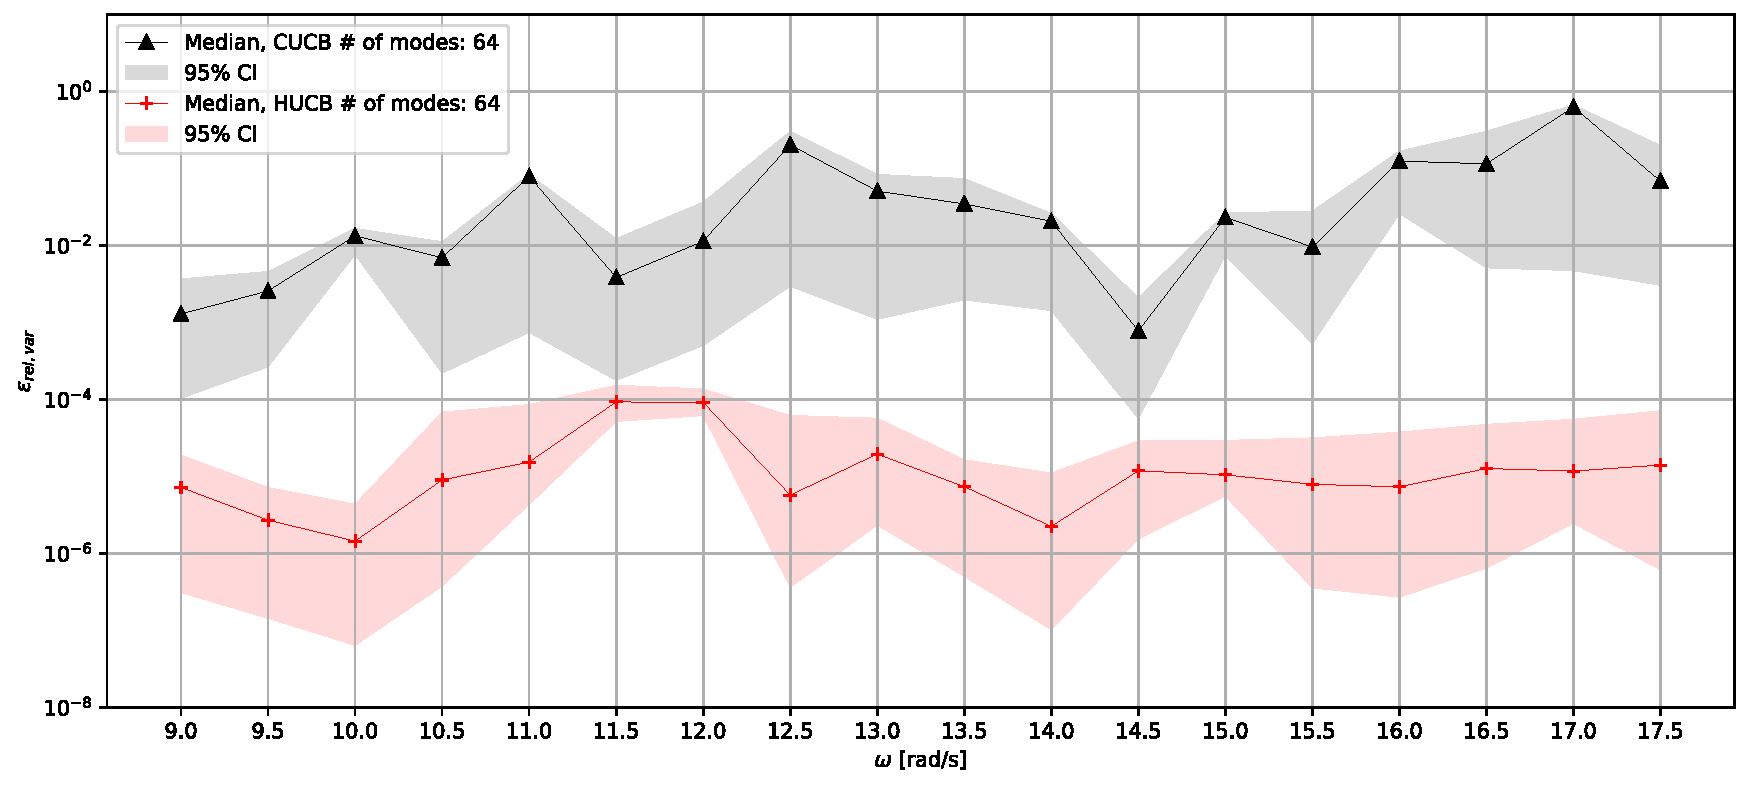
\includegraphics[width=1.0\textwidth]{
        plots/substructuring/plot_7.pdf
    }
    \caption{%
        Relative Variance Errors of $H_{AA}$ for The CUCB and HUCB Methods
    }
    \label{e_var HUCB_A_A}
\end{figure}
The two figures above show that while the relative mean errors from the two approaches are comparable, the HUCB method better approximates the FRFs' variabilities, thus leading to lower overall relative empirical error.
% -----------------------------------------------------------------------------
% Master thesis in the study program computational mechanics
%
% B.Sc. Rezha Adrian Tanuharja - 03751261
% M.Sc. Felix Schneider (supervisor)
%
% chapters/discussion/substructuring/point_B.tex
% Last edited 03 November 2023
% -----------------------------------------------------------------------------

\subsection{Vertical Acceleration at Node B}
\label{ssec: cms point B}

Figures \ref{FRF_MC_B_A_linear} and \ref{FRF_MC_B_A_log} show the vertical acceleration magnitudes at node B when a unit vertical force is present at node A.
\begin{figure}[H]
    \centering
    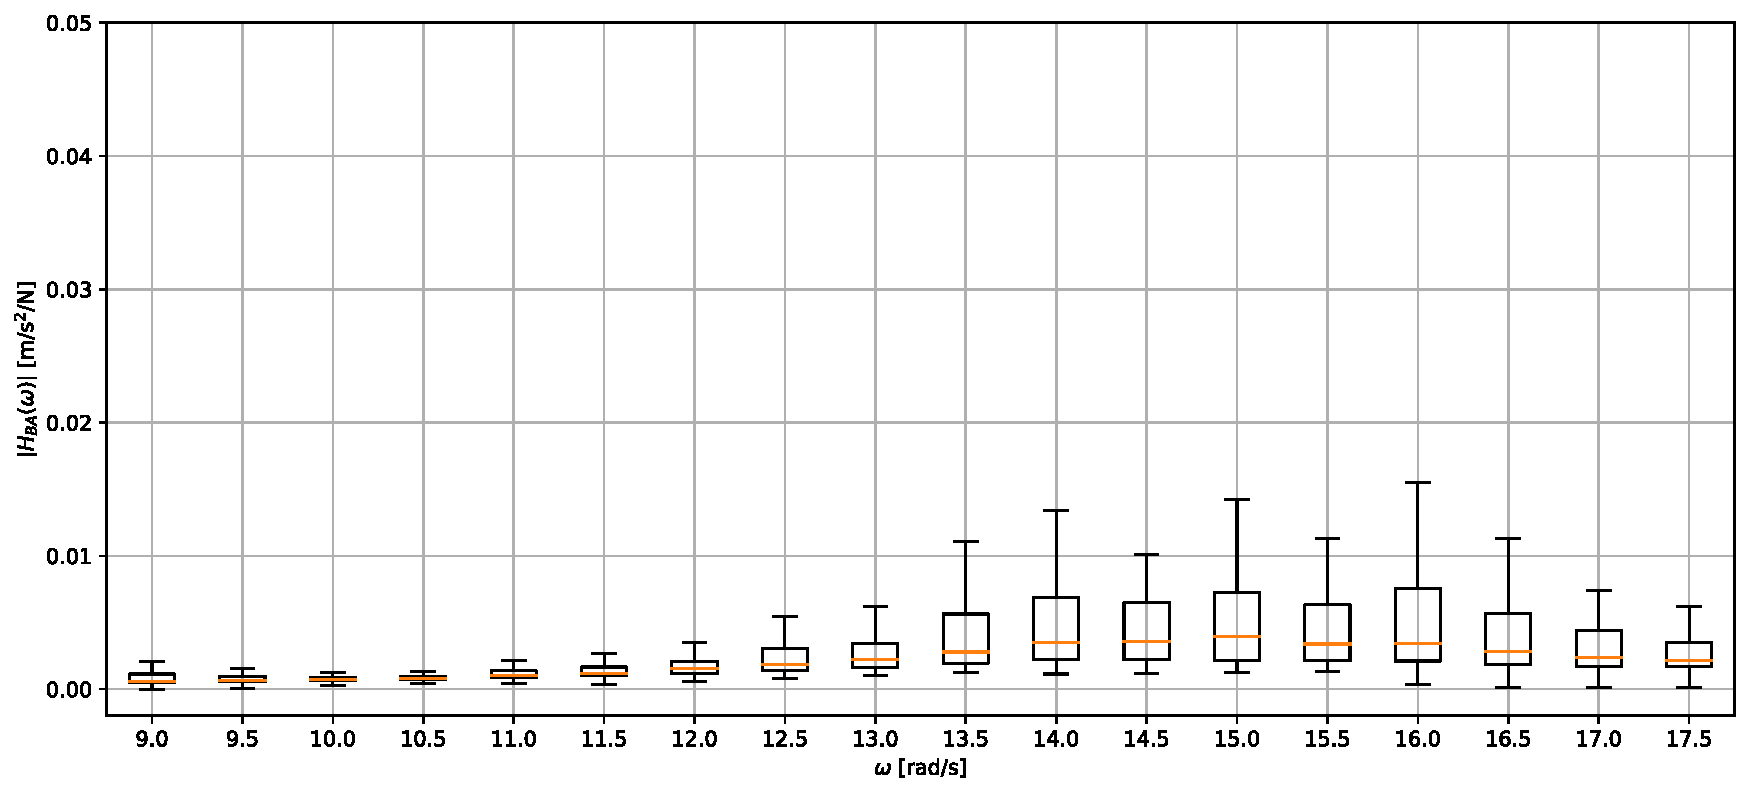
\includegraphics[width=1.0\textwidth]{
        plots/substructuring/plot_8_linear.pdf
    }
    \caption{%
        $\left|H_{BA}\right|$ from Direct MCS of The Complete Plate Model
    }
    \label{FRF_MC_B_A_linear}
\end{figure}
\begin{figure}[H]
    \centering
    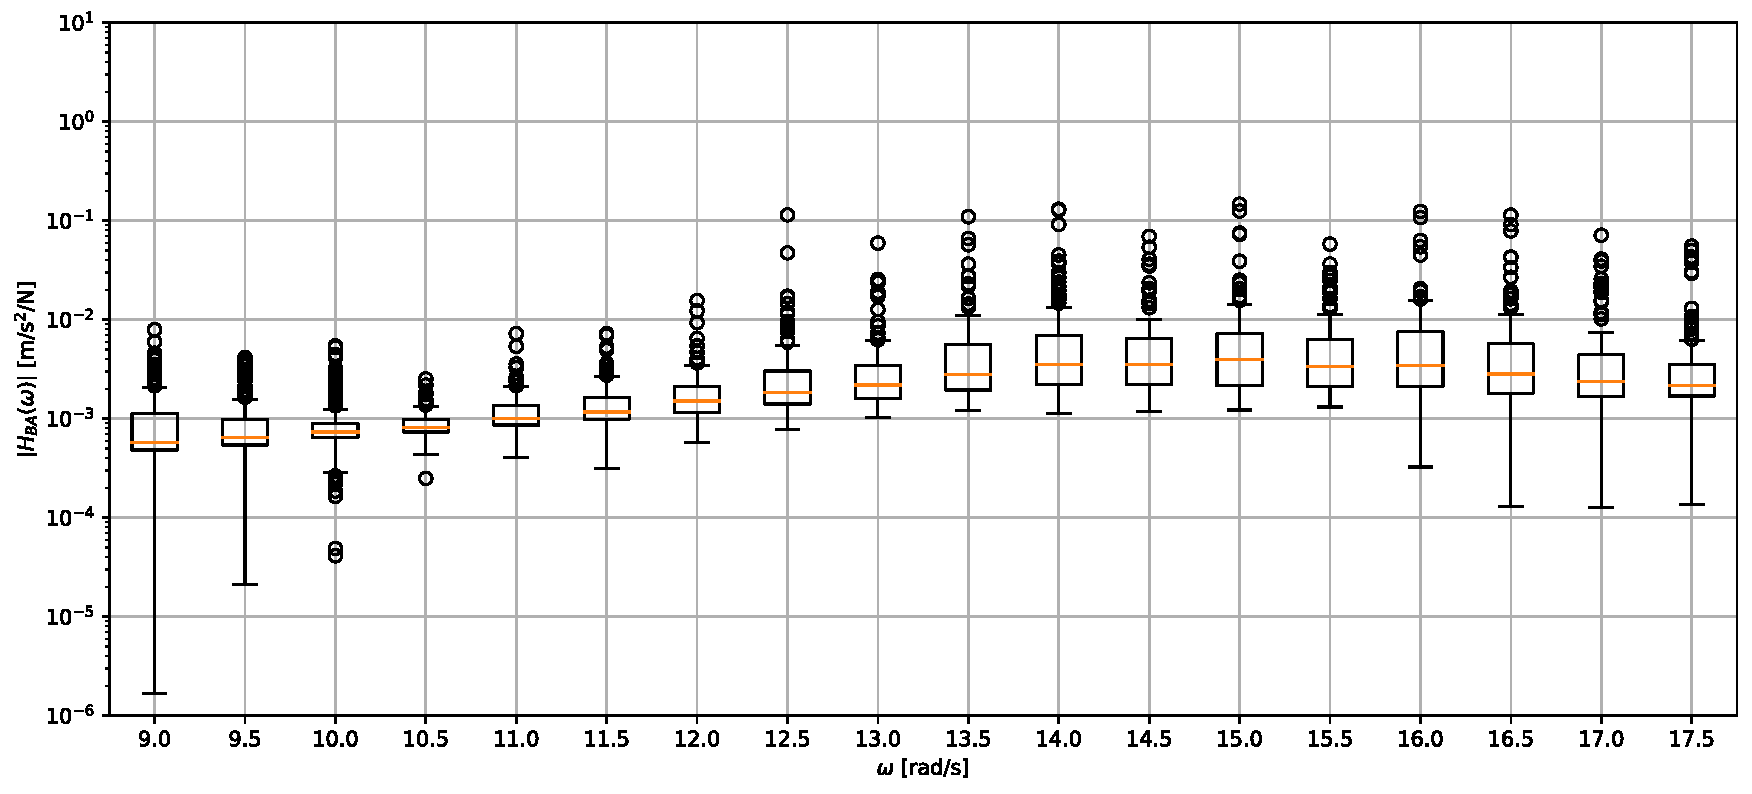
\includegraphics[width=1.0\textwidth]{
        plots/substructuring/plot_8_log.pdf
    }
    \caption{%
        $\left|H_{BA}\right|$ from Direct MCS of The Complete Plate Model with Outliers
    }
    \label{FRF_MC_B_A_log}
\end{figure}
Figure \ref{e_emp CUCB_B_A} shows the median relative empirical errors for the FRFs in each frequency in the above range using three different numbers of internal modes.
The figure exhibits a similar trend with figure \ref{e_emp CUCB_A_A}: as the number of internal modes increases, the relative empirical errors decrease.
\begin{figure}[H]
    \centering
    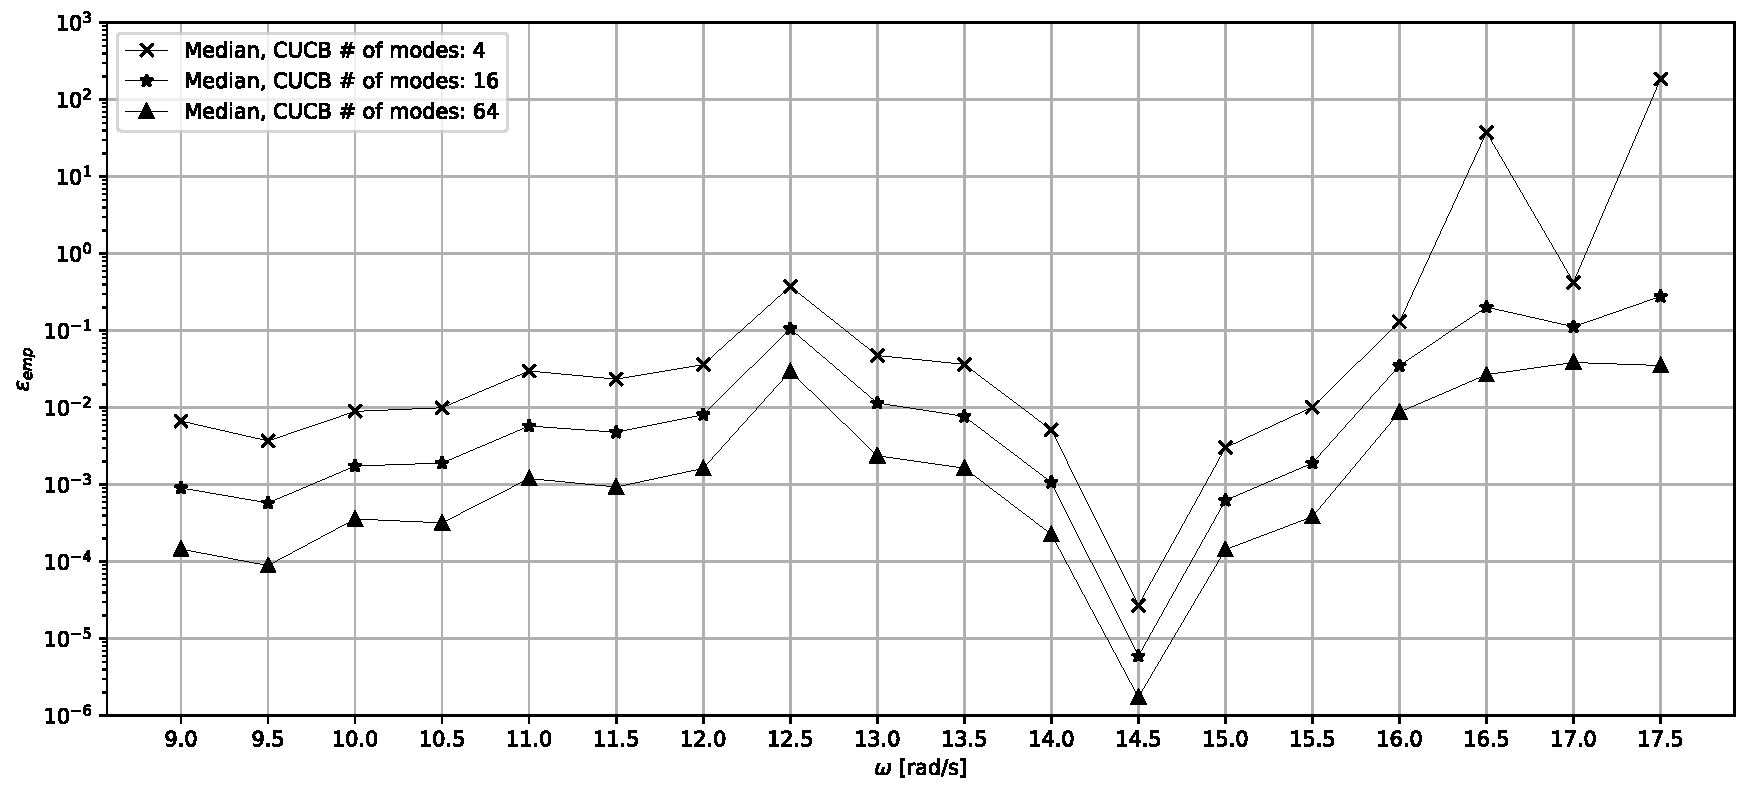
\includegraphics[width=1.0\textwidth]{
        plots/substructuring/plot_9.pdf
    }
    \caption{%
        Relative Empirical Errors of $H_{BA}$ for The CUCB Method
    }
    \label{e_emp CUCB_B_A}
\end{figure}

Figure \ref{e_emp HUCB_B_A} shows the medians and $95\%$ confidence intervals of the relative empirical errors of the FRFs' magnitudes for the crude and hybrid UCB methods.
\begin{figure}[H]
    \centering
    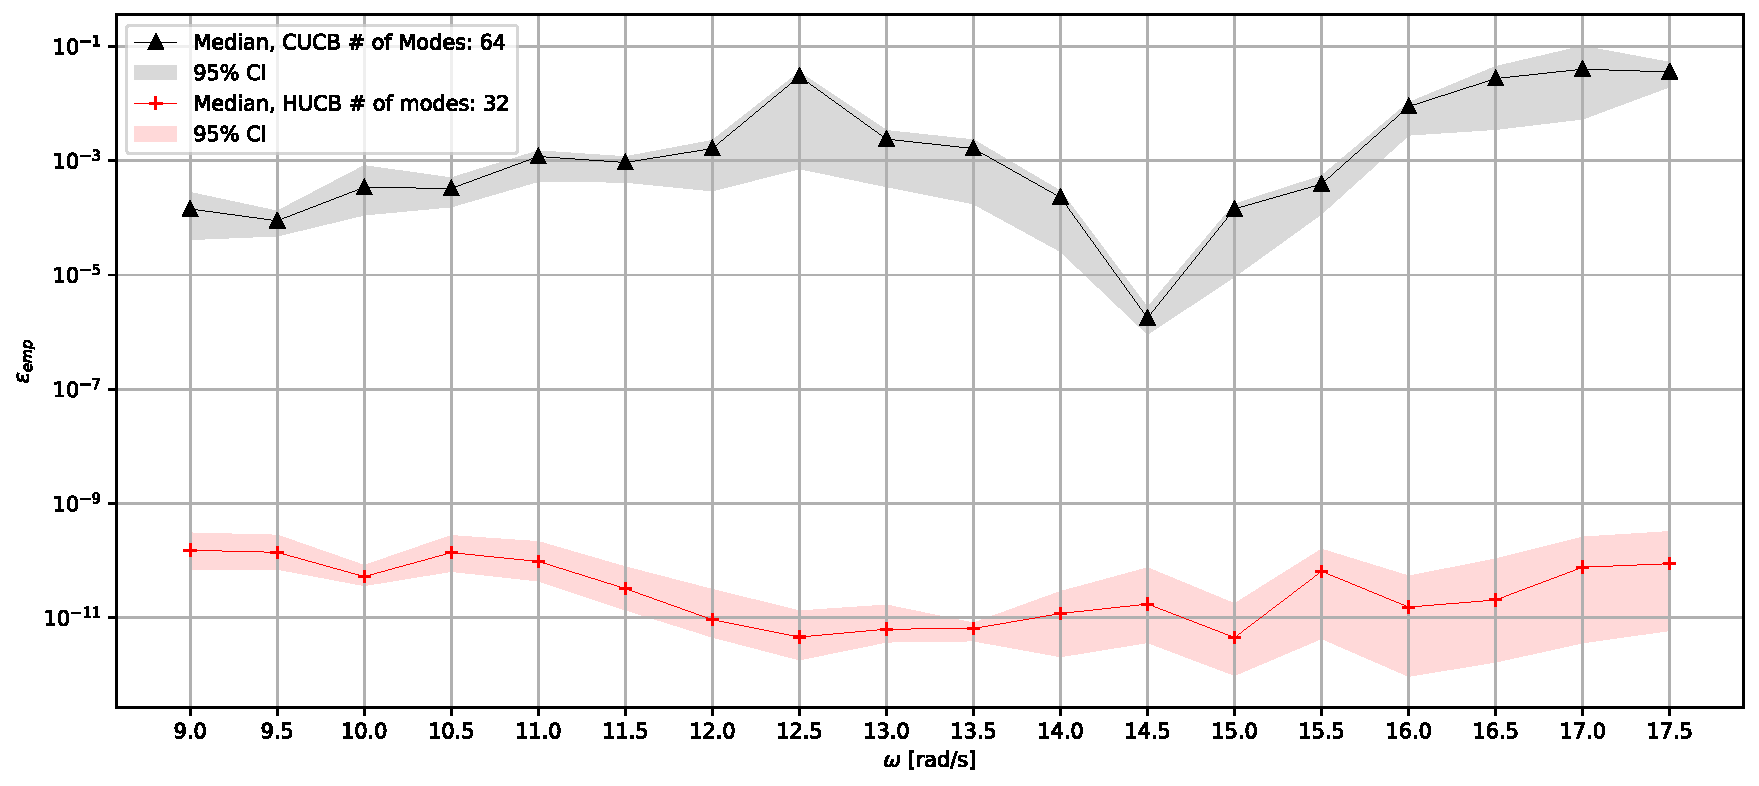
\includegraphics[width=1.0\textwidth]{
        plots/substructuring/plot_10.pdf
    }
    \caption{%
        Relative Empirical Errors of $H_{BA}$ for The CUCB and HUCB Methods
    }
    \label{e_emp HUCB_B_A}
\end{figure}
Comparing figure \ref{e_emp HUCB_A_A} with figure \ref{e_emp HUCB_B_A}, the benefit of the HUCB method over the CUCB method is more pronounced when the force and the response are at two different points or two different components.

Figure \ref{e_mean CUCB_B_A} shows the median relative mean errors of the FRFs' magnitudes for the CUCB method using three different numbers of internal modes.
\begin{figure}[H]
    \centering
    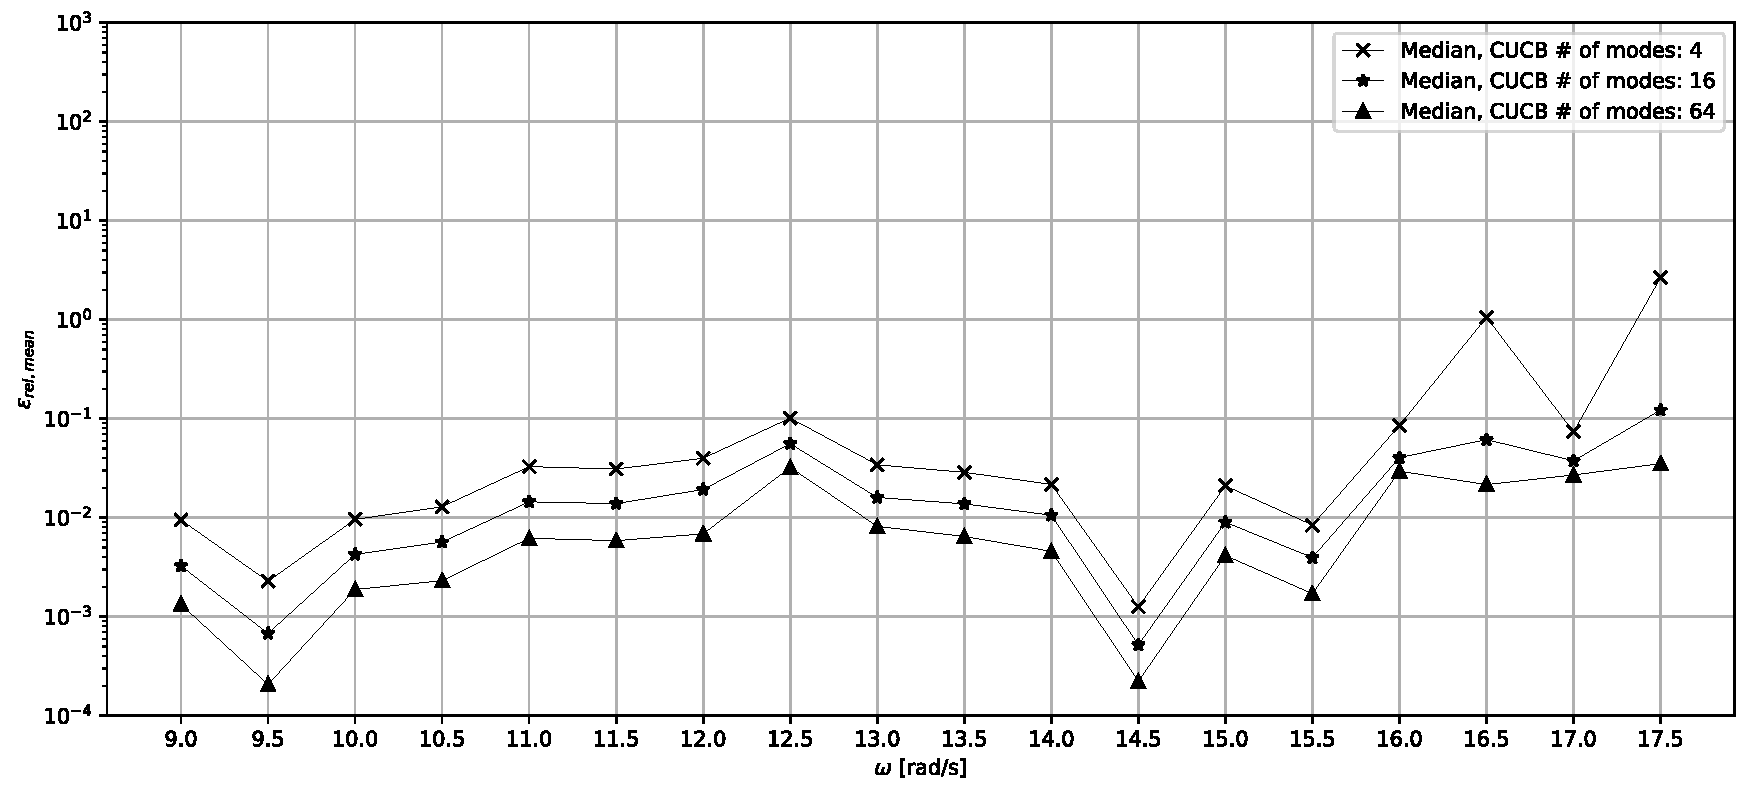
\includegraphics[width=1.0\textwidth]{
        plots/substructuring/plot_11.pdf
    }
    \caption{%
        Relative Mean Errors of $\left|H_{BA}\right|$ for The CUCB Method
    }
    \label{e_mean CUCB_B_A}
\end{figure}
Figure \ref{e_var CUCB_B_A} shows the median relative variance errors of the FRFs' magnitudes for the CUCB method using three different numbers of internal modes.
\begin{figure}[H]
    \centering
    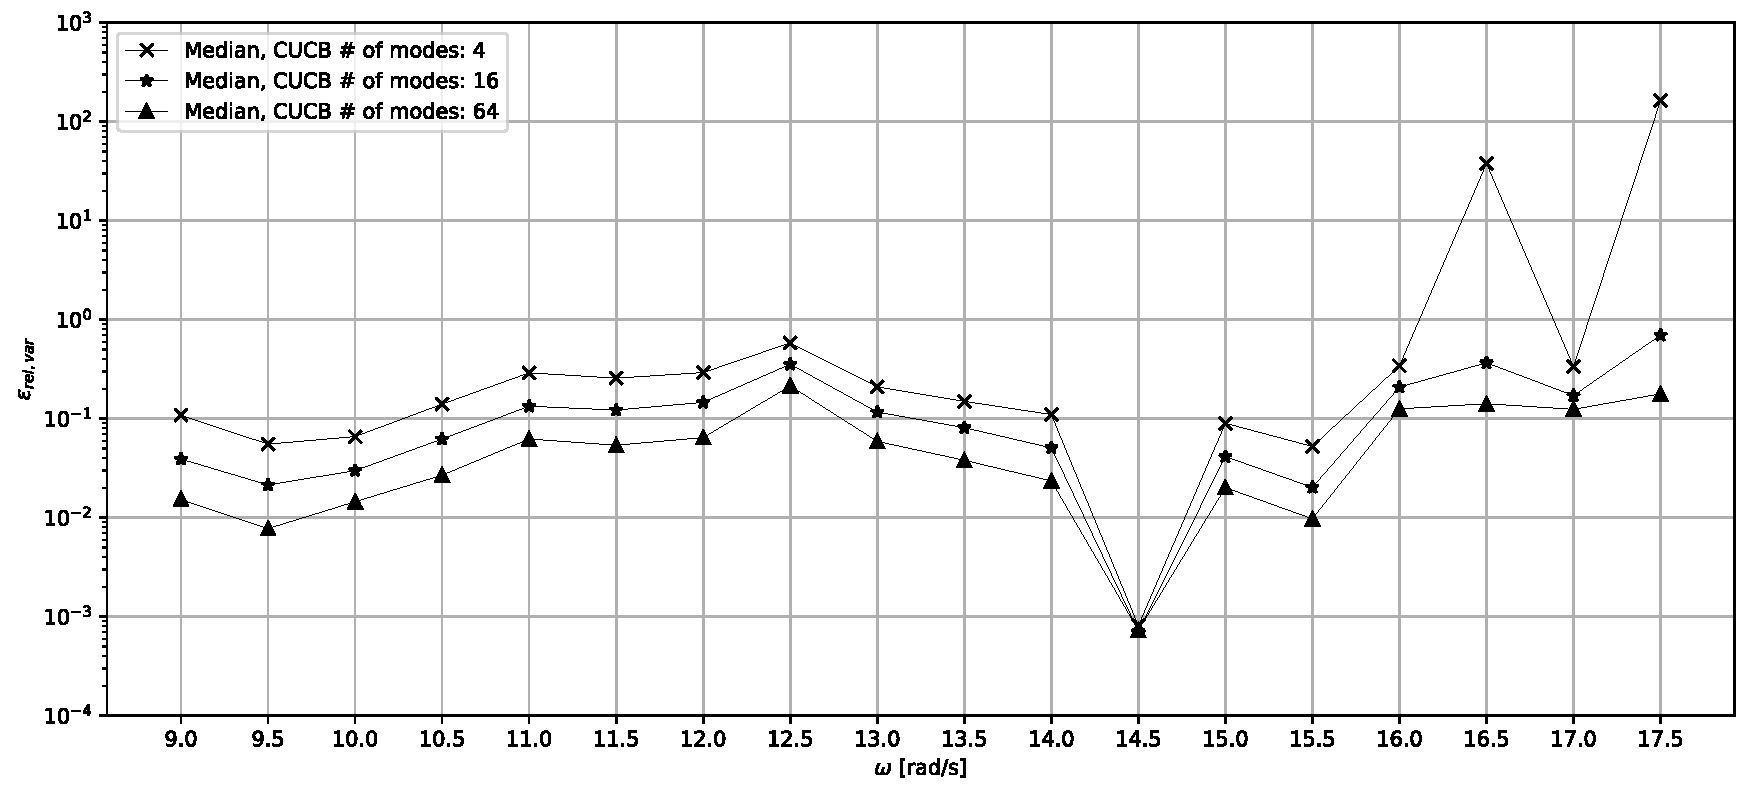
\includegraphics[width=1.0\textwidth]{
        plots/substructuring/plot_12.pdf
    }
    \caption{%
        Relative Variance Errors of $H_{BA}$ for The CUCB Method
    }
    \label{e_var CUCB_B_A}
\end{figure}
The two figures above exhibit similar trends with figure \ref{e_emp CUCB_B_A}: the relative mean errors decrease as the number of internal modes increases.
Overall, the relative mean errors are lower than the relative variance errors.

Figure \ref{e_mean HUCB_B_A} shows the medians and $95\%$ confidence intervals of the relative mean errors for the crude and hybrid UCB methods.
\begin{figure}[H]
    \centering
    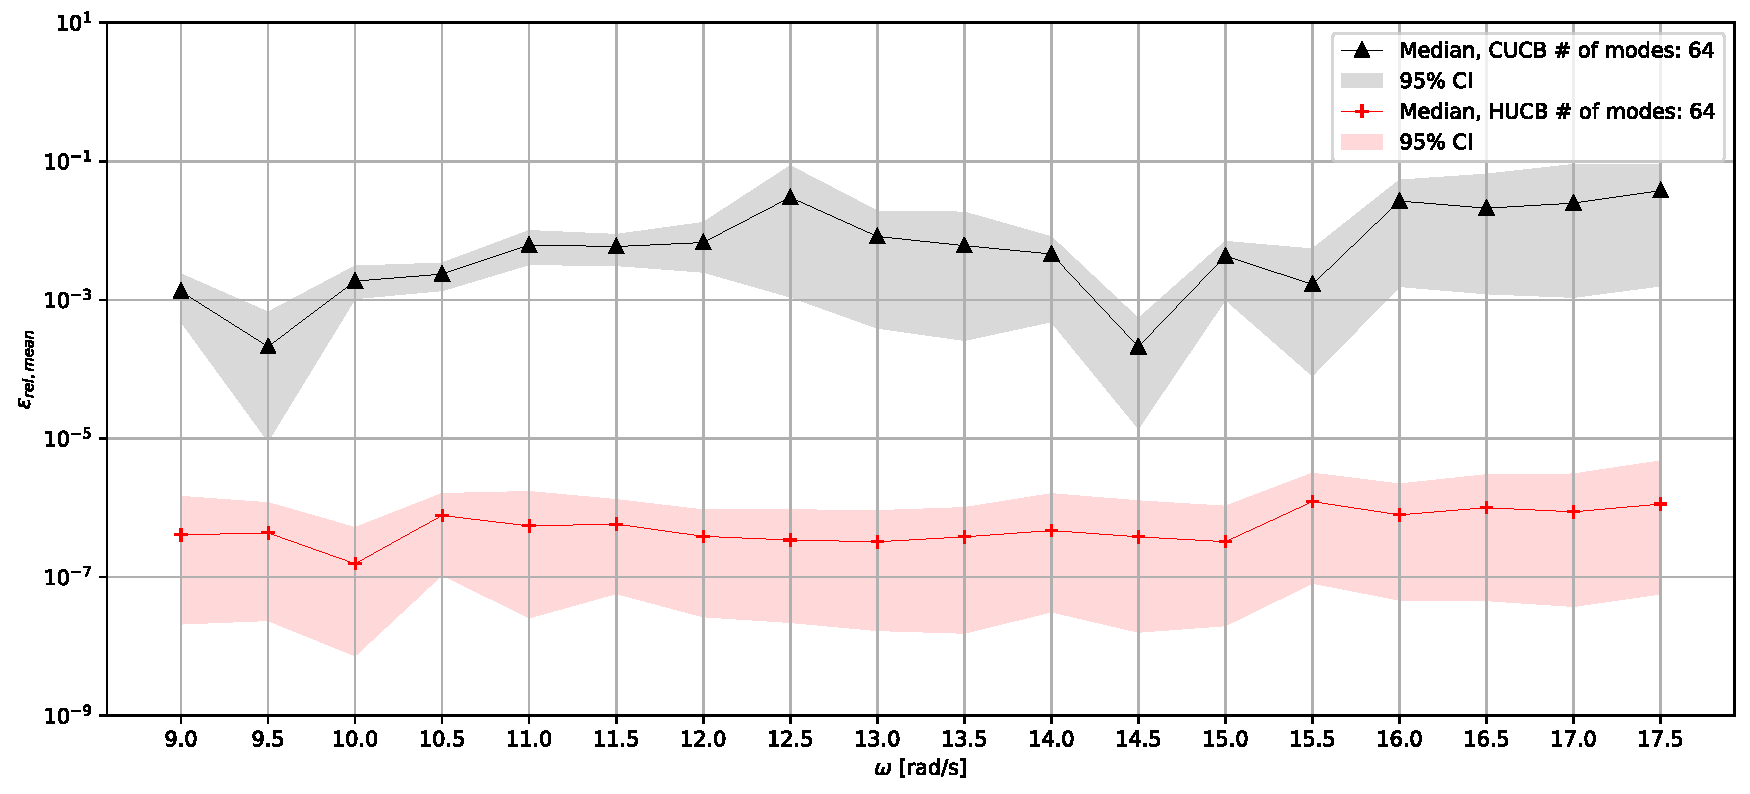
\includegraphics[width=1.0\textwidth]{
        plots/substructuring/plot_13.pdf
    }
    \caption{%
        Relative Mean Errors of $\left|H_{BA}\right|$ for The CUCB and HUCB Methods
    }
    \label{e_mean HUCB_B_A}
\end{figure}
Figure \ref{e_var HUCB_B_A} shows the medians and $95\%$ confidence intervals of the relative variance errors for the crude and hybrid UCB methods.
\begin{figure}[H]
    \centering
    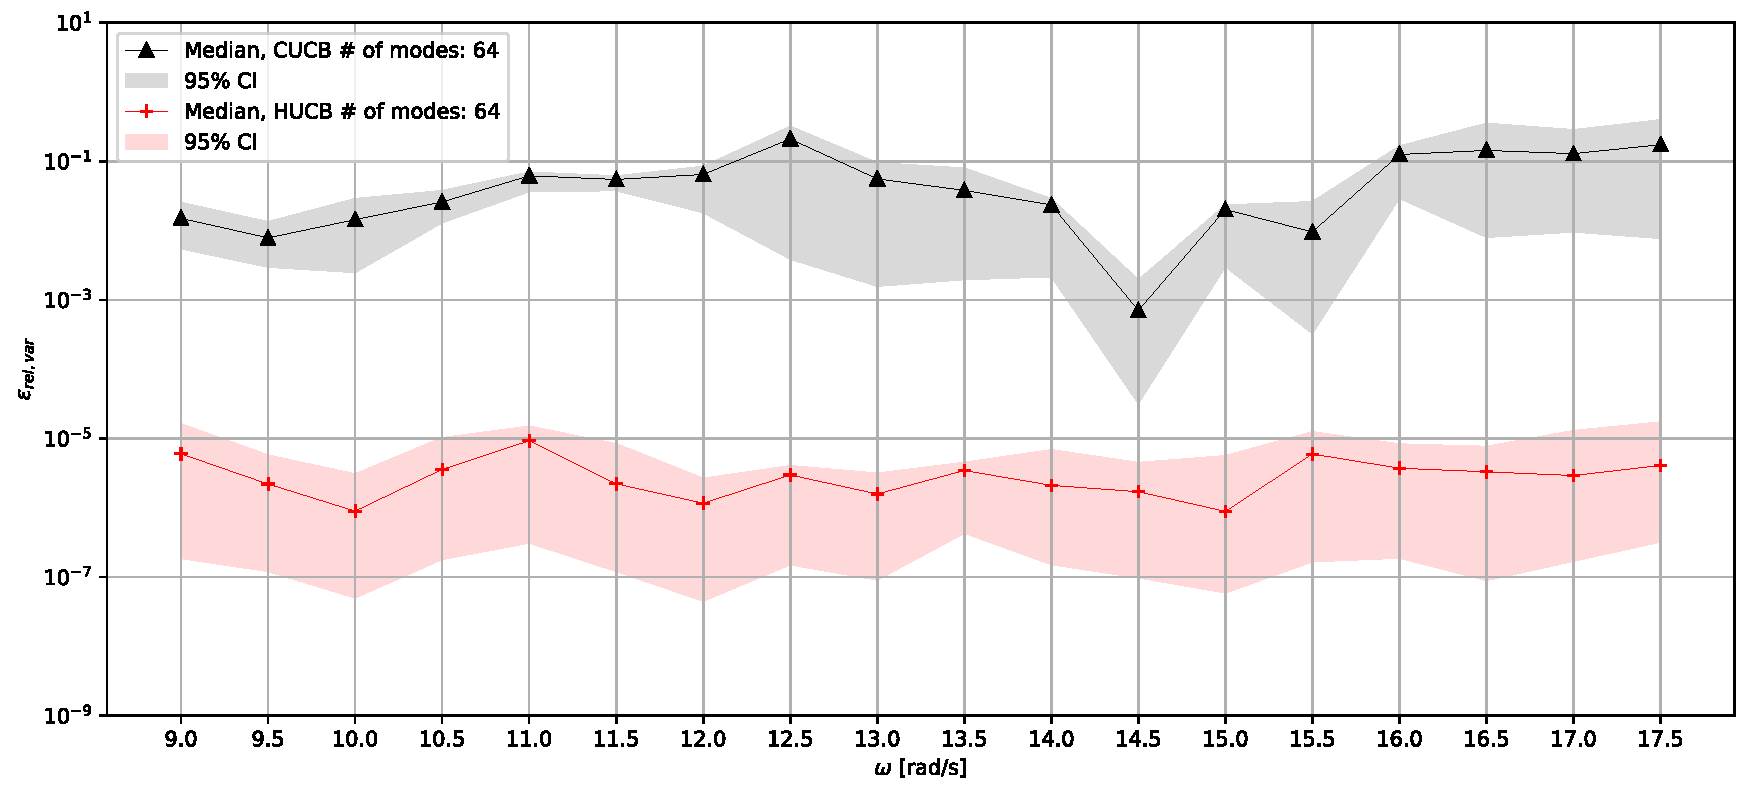
\includegraphics[width=1.0\textwidth]{
        plots/substructuring/plot_14.pdf
    }
    \caption{%
        Relative Variance Errors of $H_{BA}$ for The CUCB and HUCB Methods
    }
    \label{e_var HUCB_B_A}
\end{figure}
The two figures above show that both the relative mean errors and relative variance errors are lower when using the hybrid UCB method by several orders of magnitude.
% -----------------------------------------------------------------------------
% Master thesis in the study program computational mechanics
%
% B.Sc. Rezha Adrian Tanuharja - 03751261
% M.Sc. Felix Schneider (supervisor)
%
% chapters/discussion/surrogate.tex
% Last edited 03 November 2023
% -----------------------------------------------------------------------------

\section{Performance of Surrogate Models}
\label{sec: performance of surrogate models}

This section reports the findings from the second half of the proposed framework: the surrogate modeling part.
These findings come from observing the plate's vertical acceleration at nodes A and B when subjected to a unit vertical force at node A.
Details about the nodes are available in chapter \ref{ch: methodology}.

% -----------------------------------------------------------------------------
% Master thesis in the study program computational mechanics
%
% B.Sc. Rezha Adrian Tanuharja - 03751261
% M.Sc. Felix Schneider (supervisor)
%
% chapters/discussion/substructuring/point_A.tex
% Last edited 03 November 2023
% -----------------------------------------------------------------------------

\subsection{Vertical Acceleration at Node A}
\label{ssec: cms point A}

Figure \ref{FRF_MC_A_A_linear} shows the FRFs from direct MCS of the complete plate model.
These FRFs relate the vertical acceleration magnitude at point A to a unit force at the same point at discrete frequencies in the range $\left[9.0, 17.5\right]$ rad/s with increments of $0.5$ rad/s.
The outliers are intentionally missing to enable a clear view of the FRFs' statistics: their medians, interquartile ranges, and whiskers.
\begin{figure}[H]
    \centering
    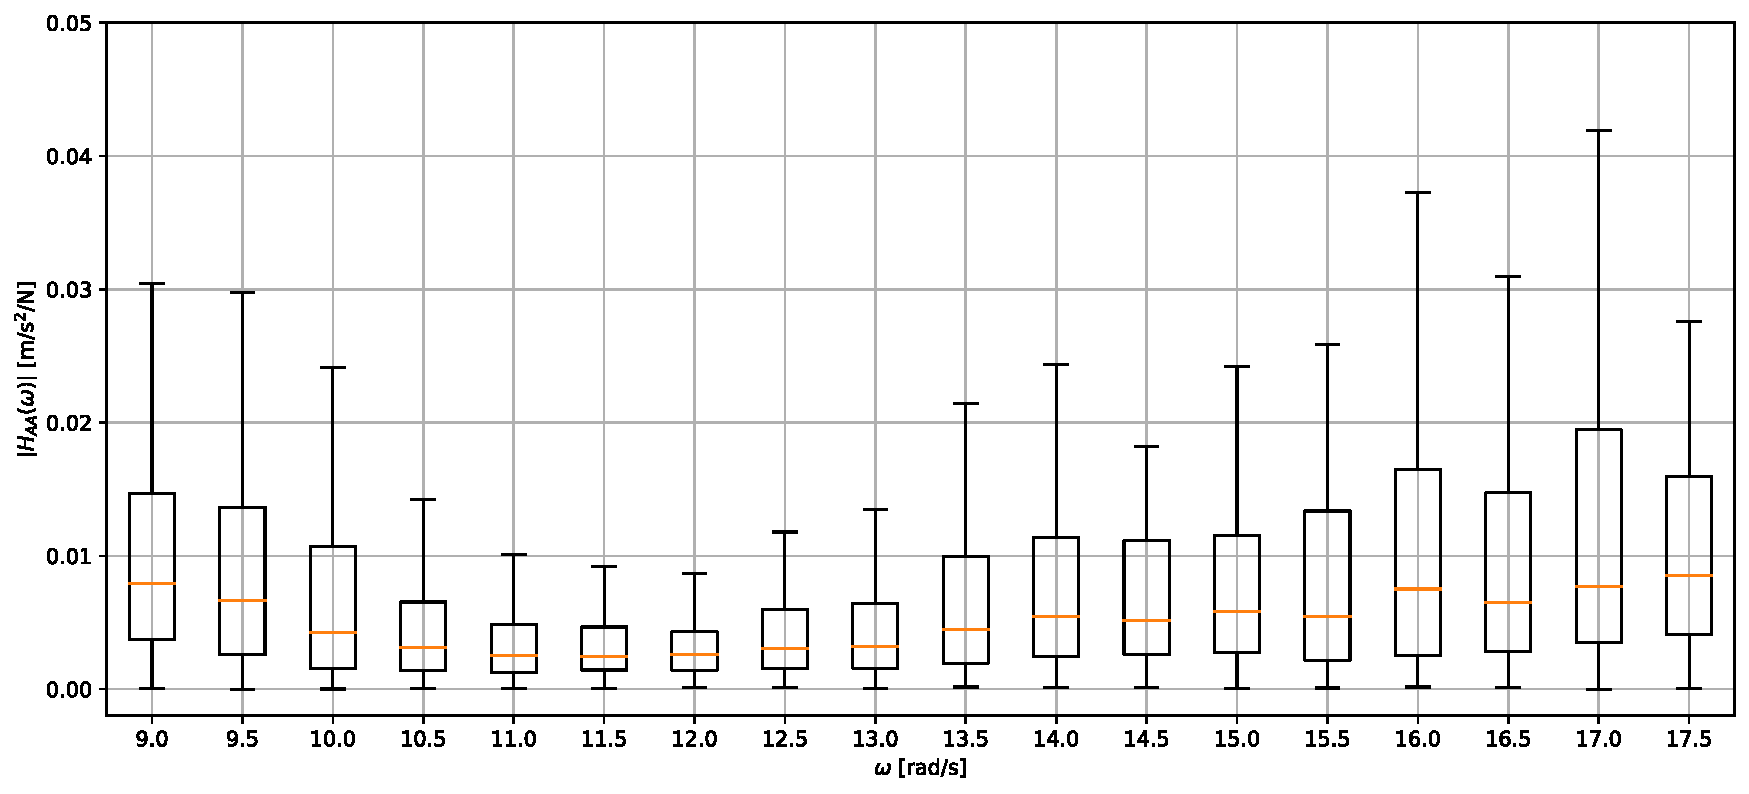
\includegraphics[width=1.0\textwidth]{
        plots/substructuring/plot_1_linear.pdf
    }
    \caption{%
        $\left|H_{AA}\right|$ from Direct MCS of The Complete Plate Model
    }
    \label{FRF_MC_A_A_linear}
\end{figure}
Figure \ref{FRF_MC_A_A_log} shows the same FRFs as figure \ref{FRF_MC_A_A_linear} with outliers.
The logarithmic scale provides a clear view of the outliers and the low whiskers of the plot.
The figure shows that the outlier values can be larger by approximately two orders of magnitudes compared to the medians.
\begin{figure}[H]
    \centering
    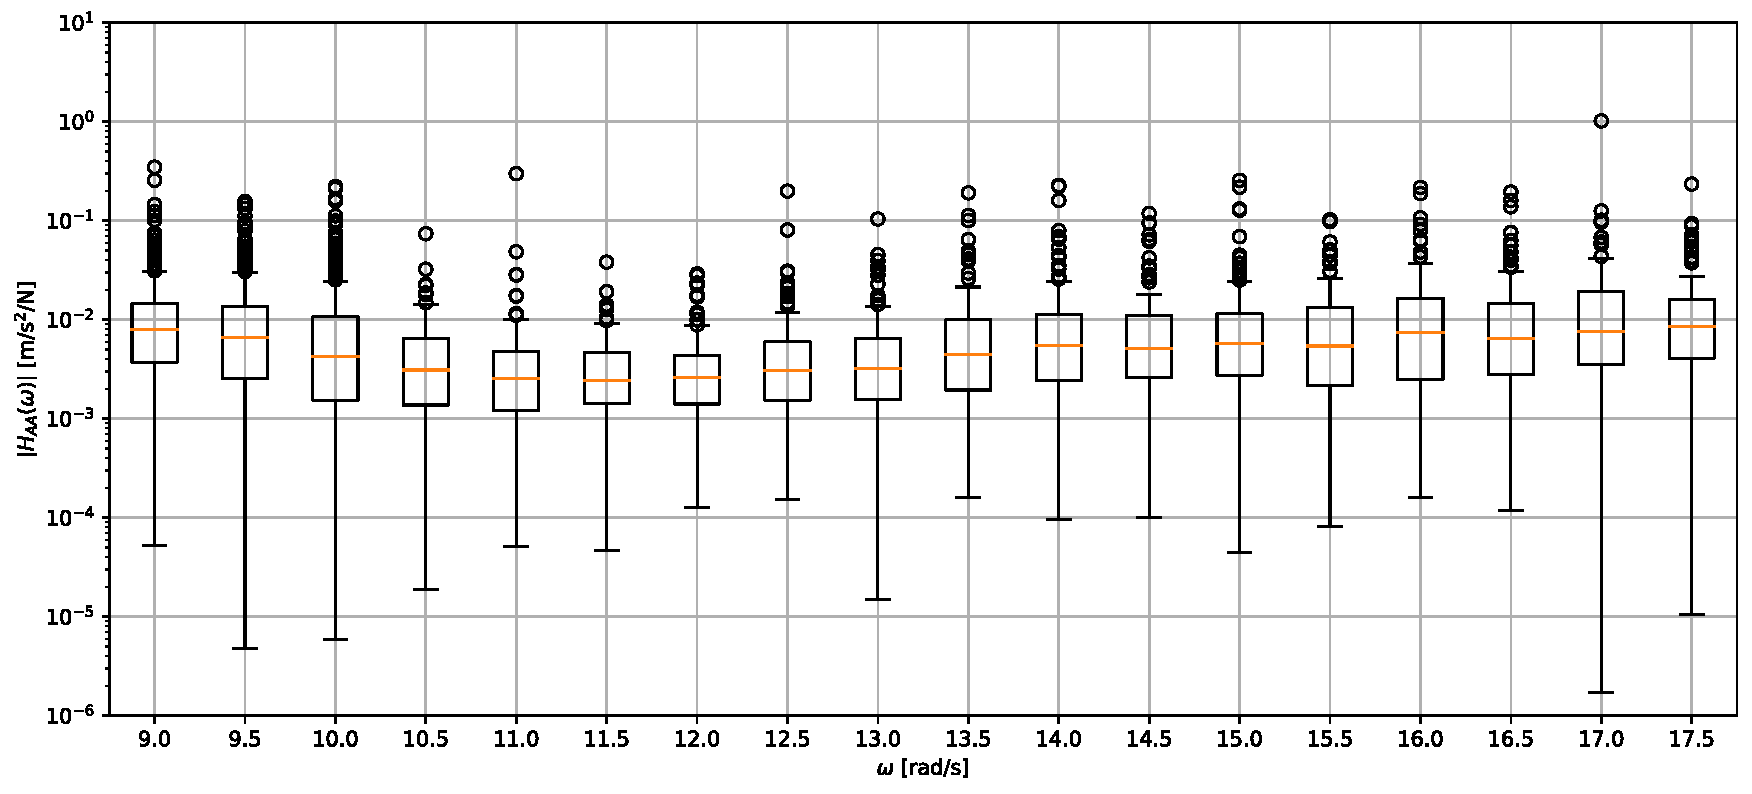
\includegraphics[width=1.0\textwidth]{
        plots/substructuring/plot_1_log.pdf
    }
    \caption{%
        $\left|H_{AA}\right|$ from Direct MCS of The Complete Plate Model with Outliers
    }
    \label{FRF_MC_A_A_log}
\end{figure}
First, the author analyzes the performance of the CUCB method.
Figure \ref{e_emp CUCB_A_A} shows the median relative empirical errors for the method in each frequency in the above range using three different numbers of internal modes.
The medians come from the bootstrapping method with a $1000$ number of resamplings.
\begin{figure}[H]
    \centering
    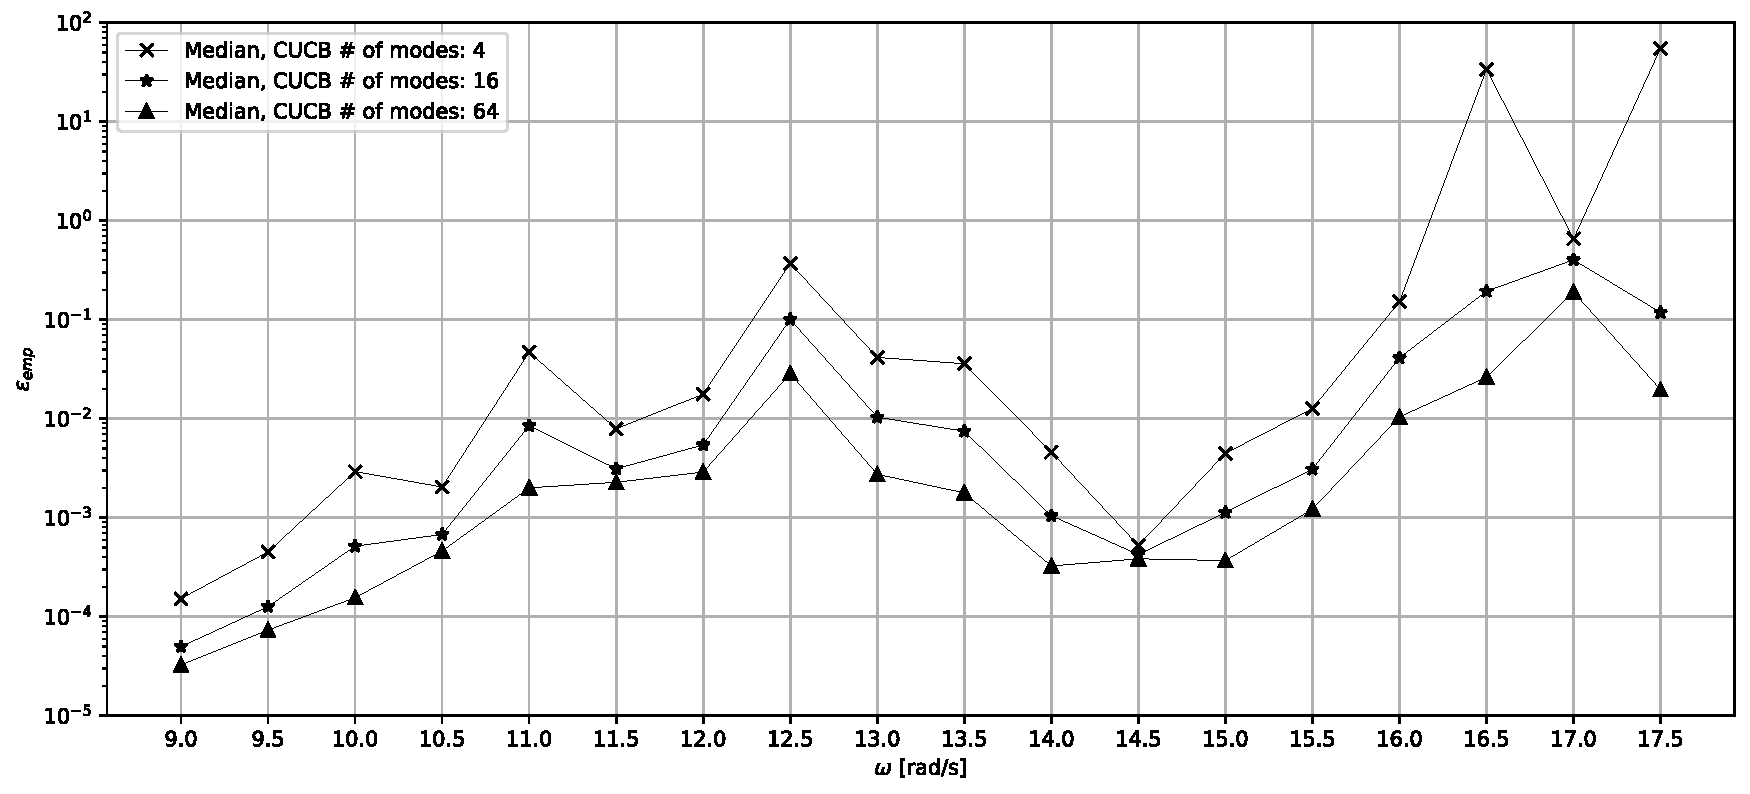
\includegraphics[width=1.0\textwidth]{
        plots/substructuring/plot_2.pdf
    }
    \caption{%
        Relative Empirical Errors of $H_{AA}$ for The CUCB Method
    }
    \label{e_emp CUCB_A_A}
\end{figure}
In deterministic dynamic substructuring, errors decrease as the number of internal modes increases.
When all internal modes are present in the model, the assembled components are equivalent to the complete structure in a mathematical sense.
Figure \ref{e_emp CUCB_A_A} exhibits the same trend for dynamic structuring using the CUCB method: as the number of internal modes increases, the relative empirical errors decrease.
However, the relative empirical errors exceeds $10^{-1}$ at $\omega=17.0$ rad/s even when using $64$ internal modes.
Therefore, the mean square errors are in the same order of magnitude as the FRFs' variance at this frequency.

Subsequently, the author analyzes the performance of the HUCB method.
Figure \ref{e_emp HUCB_A_A} shows the medians and $95\%$ confidence intervals of the relative empirical errors for the crude and hybrid UCB methods.
Figure \ref{e_emp HUCB_A_A} shows that the relative empirical errors from the HUCB method do not exceed $10^{-2}$ in this example and in most frequencies in the range lie below $10^{-3}$.
The computational cost of the HUCB method is higher than that of the CUCB method because of the evaluation of the boundary modes for each input parameter's realization.
However, it leads to lower overall relative empirical errors and, in some frequencies, reduces the errors by up to two orders of magnitudes.
\begin{figure}[H]
    \centering
    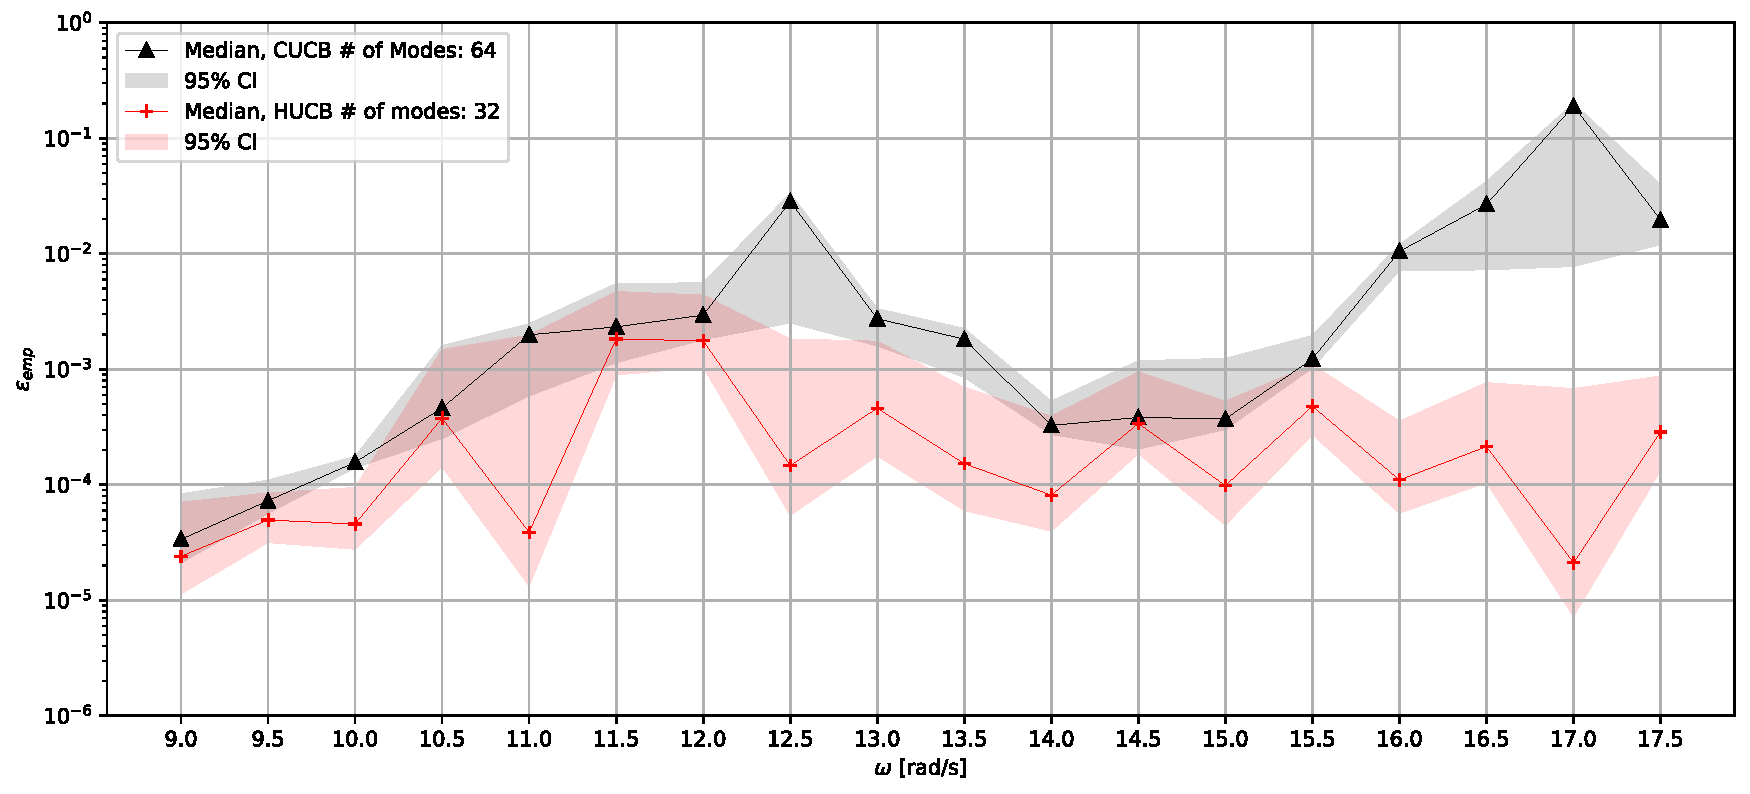
\includegraphics[width=1.0\textwidth]{
        plots/substructuring/plot_3.pdf
    }
    \caption{%
        Relative Empirical Errors of $H_{AA}$ for The CUCB and HUCB Methods
    }
    \label{e_emp HUCB_A_A}
\end{figure}

To dive deeper into the difference between the crude and hybrid UCB methods, the author evaluates the relative mean and variance errors.
Figure \ref{e_mean CUCB_A_A} shows the median relative mean errors of the FRFs' magnitudes for the CUCB method using three different numbers of internal modes.
\begin{figure}[H]
    \centering
    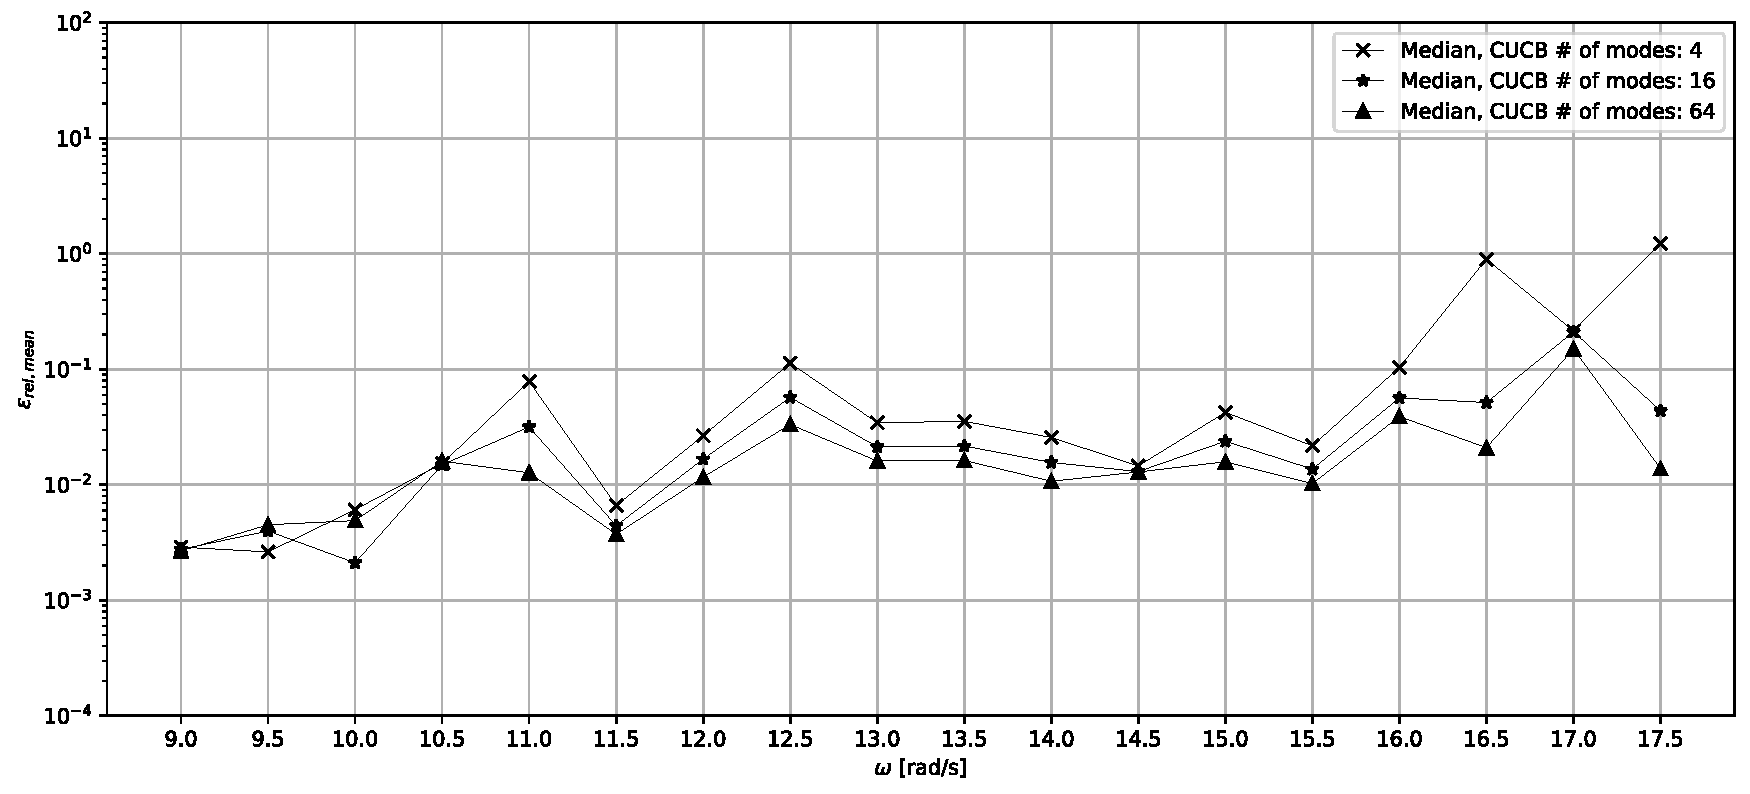
\includegraphics[width=1.0\textwidth]{
        plots/substructuring/plot_4.pdf
    }
    \caption{%
        Relative Mean Errors of $\left|H_{AA}\right|$ for The CUCB Method
    }
    \label{e_mean CUCB_A_A}
\end{figure}
Figure \ref{e_var CUCB_A_A} shows the median relative variance errors of the FRFs for the CUCB method using three different numbers of internal modes.
\begin{figure}[H]
    \centering
    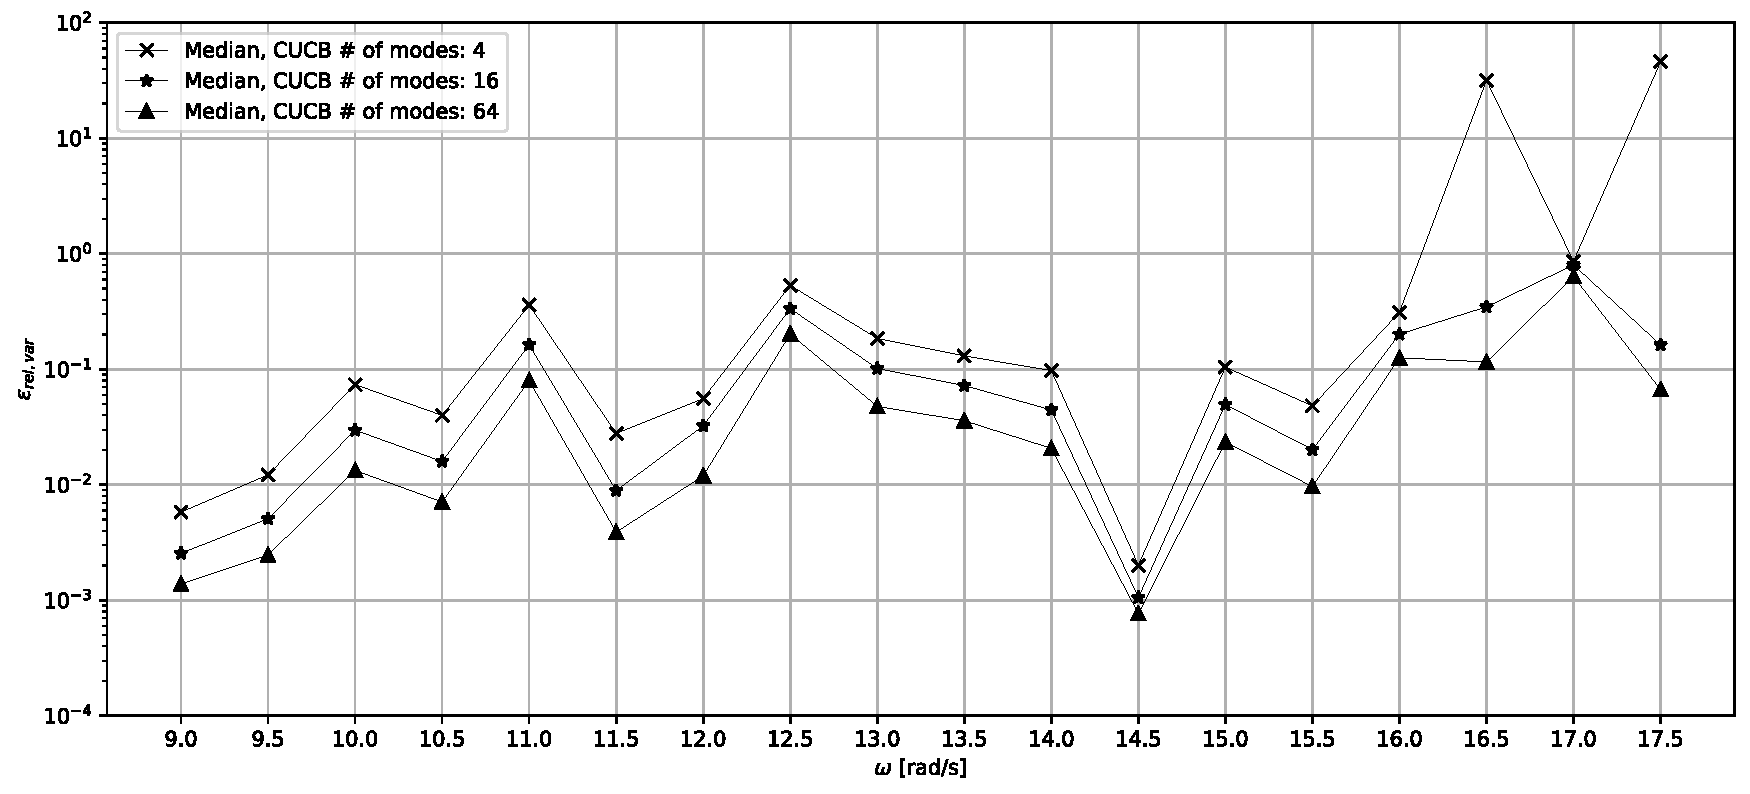
\includegraphics[width=1.0\textwidth]{
        plots/substructuring/plot_5.pdf
    }
    \caption{%
        Relative Variance Errors of $H_{AA}$ for The CUCB Method
    }
    \label{e_var CUCB_A_A}
\end{figure}
The two figures above exhibit similar trends with figure \ref{e_emp CUCB_A_A}: the relative mean errors decrease as the number of internal modes increases, with an exception at $\omega=9.5$ rad/s for the relative mean errors.
Overall, the relative mean errors and relative variance errors primarily lie between $10^{-3}$ and $10^{0}$.

Subsequently, the author compares the relative mean errors and relative variance errors for the CUCB method and the HUCB method.
Figure \ref{e_mean HUCB_A_A} shows the medians and $95\%$ confidence intervals of the relative mean errors of the FRFs' magnitudes in each frequency in the above range for the crude and hybrid UCB methods.
\begin{figure}[H]
    \centering
    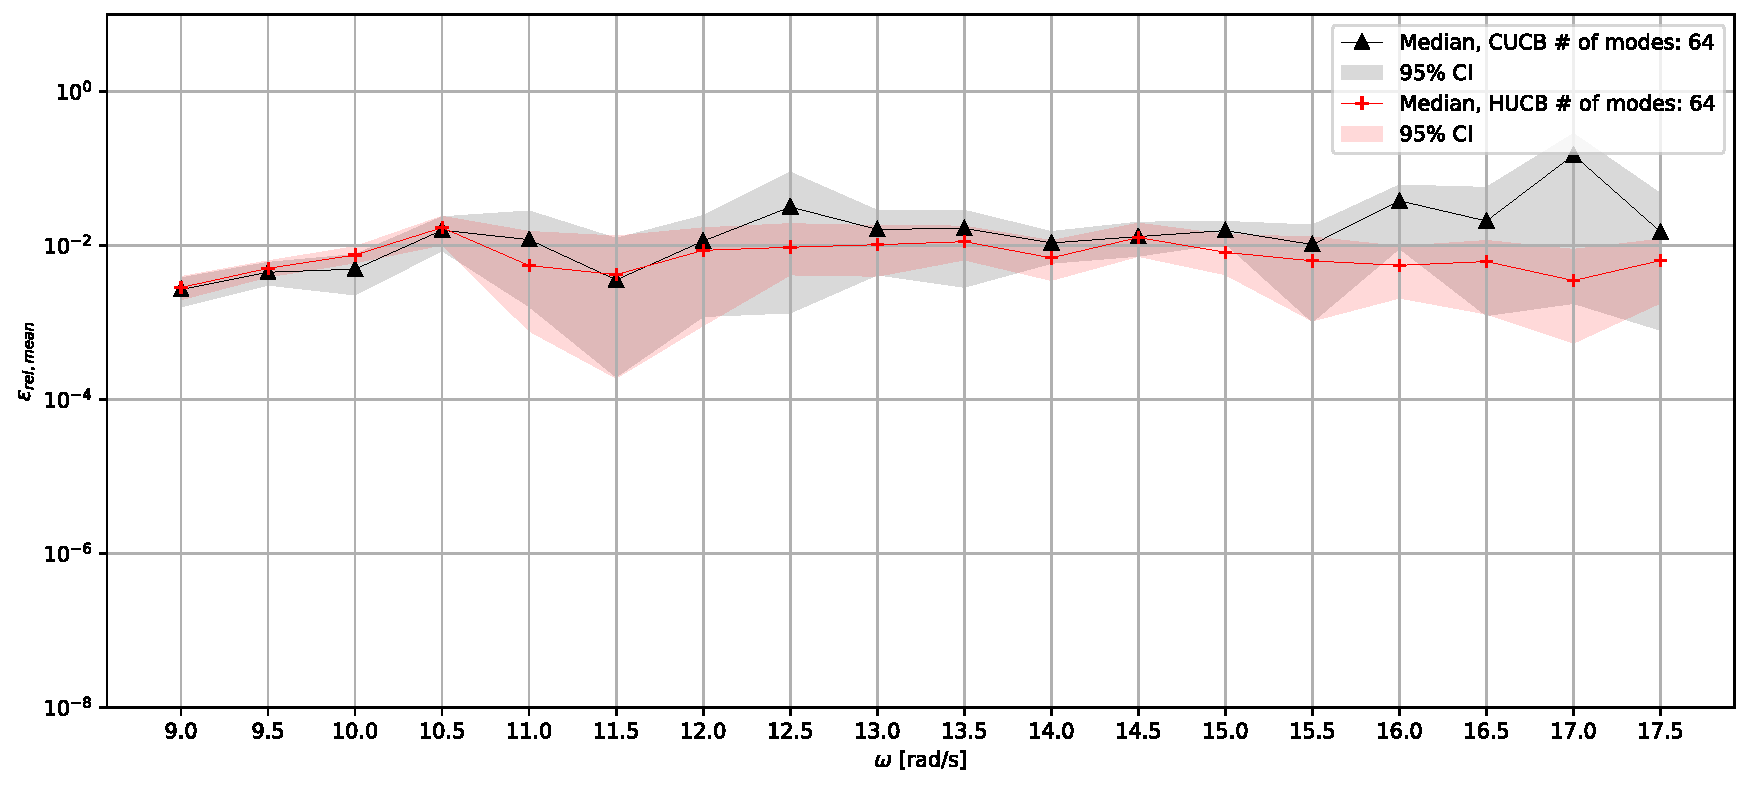
\includegraphics[width=1.0\textwidth]{
        plots/substructuring/plot_6.pdf
    }
    \caption{%
        Relative Mean Errors of $\left|H_{AA}\right|$ for The CUCB and HUCB Methods
    }
    \label{e_mean HUCB_A_A}
\end{figure}
Figure \ref{e_var HUCB_A_A} shows the median and $95\%$ confidence interval of the relative variance error for the FRFs' magnitudes in each frequency in the above range using the crude and hybrid UCB methods.
\begin{figure}[H]
    \centering
    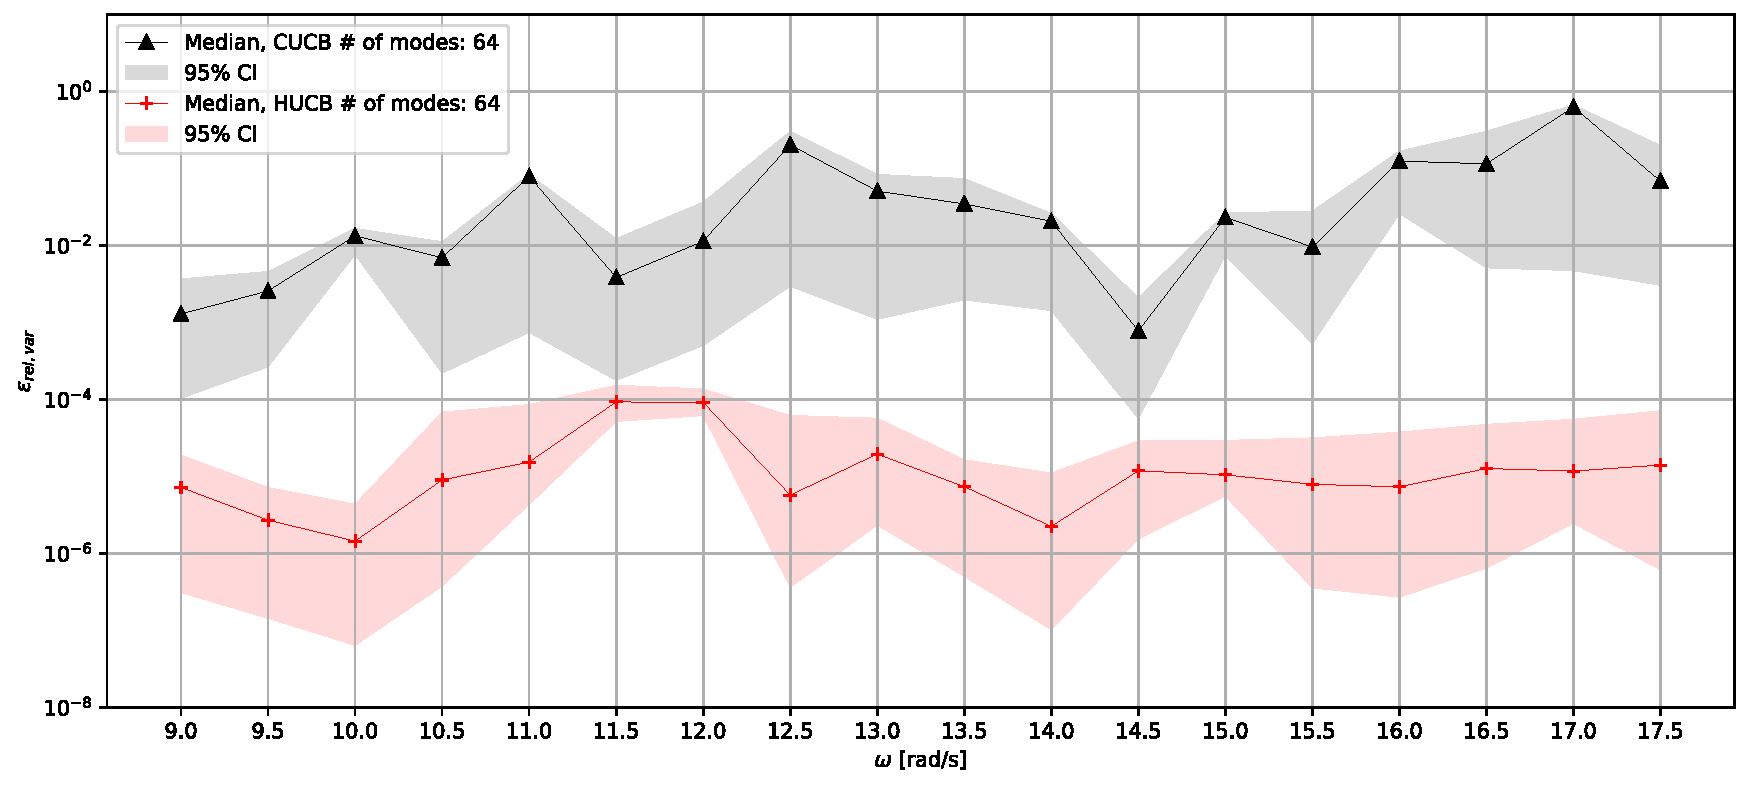
\includegraphics[width=1.0\textwidth]{
        plots/substructuring/plot_7.pdf
    }
    \caption{%
        Relative Variance Errors of $H_{AA}$ for The CUCB and HUCB Methods
    }
    \label{e_var HUCB_A_A}
\end{figure}
The two figures above show that while the relative mean errors from the two approaches are comparable, the HUCB method better approximates the FRFs' variabilities, thus leading to lower overall relative empirical error.
% -----------------------------------------------------------------------------
% Master thesis in the study program computational mechanics
%
% B.Sc. Rezha Adrian Tanuharja - 03751261
% M.Sc. Felix Schneider (supervisor)
%
% chapters/discussion/substructuring/point_B.tex
% Last edited 03 November 2023
% -----------------------------------------------------------------------------

\subsection{Vertical Acceleration at Node B}
\label{ssec: cms point B}

Figures \ref{FRF_MC_B_A_linear} and \ref{FRF_MC_B_A_log} show the vertical acceleration magnitudes at node B when a unit vertical force is present at node A.
\begin{figure}[H]
    \centering
    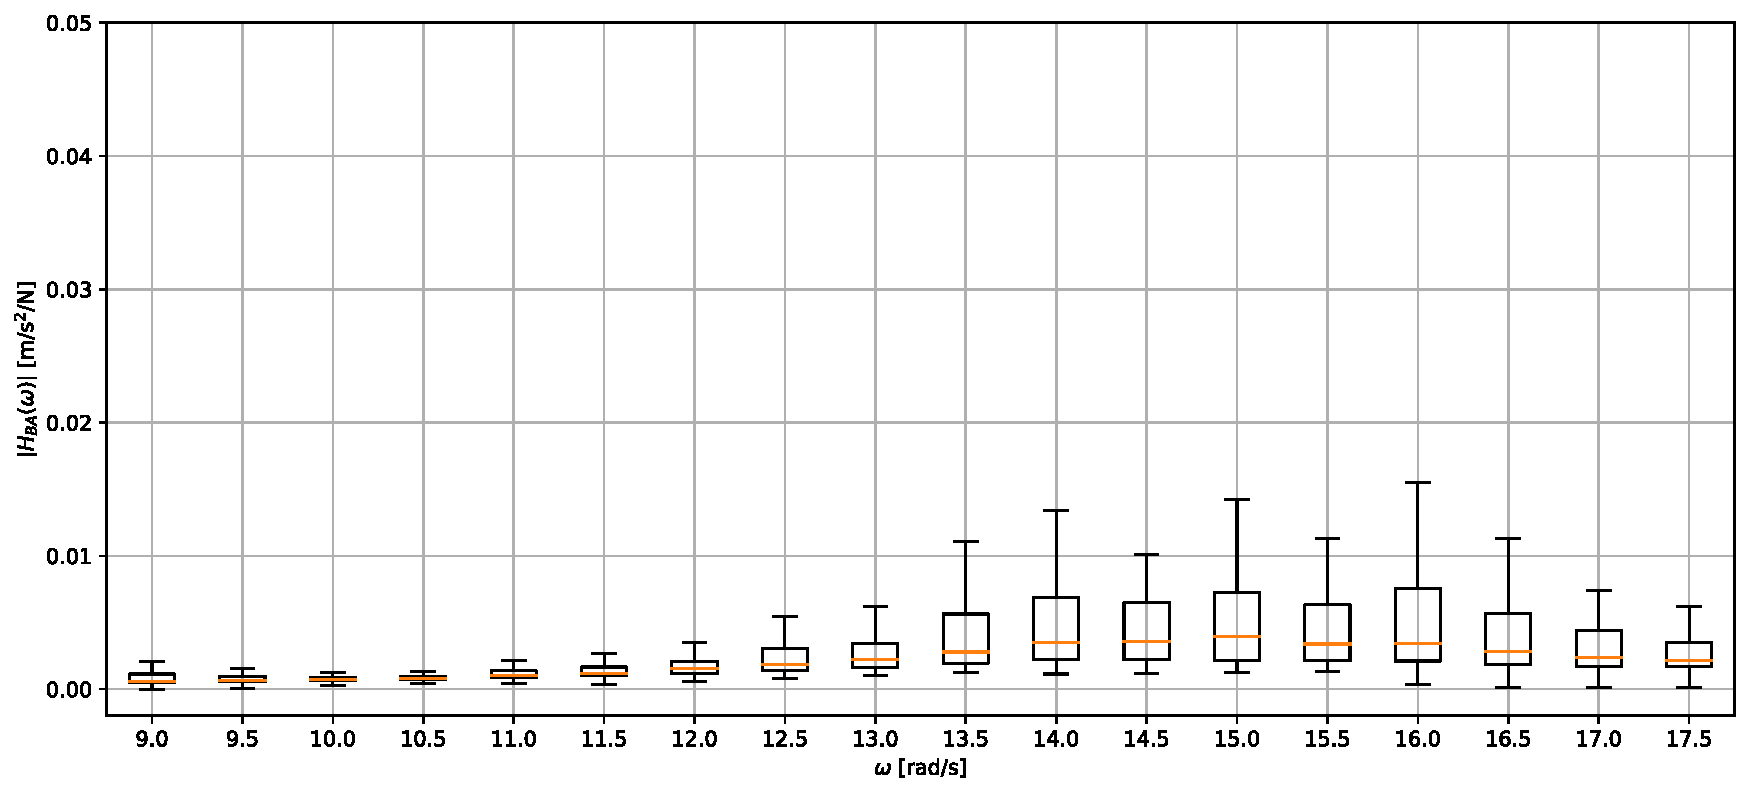
\includegraphics[width=1.0\textwidth]{
        plots/substructuring/plot_8_linear.pdf
    }
    \caption{%
        $\left|H_{BA}\right|$ from Direct MCS of The Complete Plate Model
    }
    \label{FRF_MC_B_A_linear}
\end{figure}
\begin{figure}[H]
    \centering
    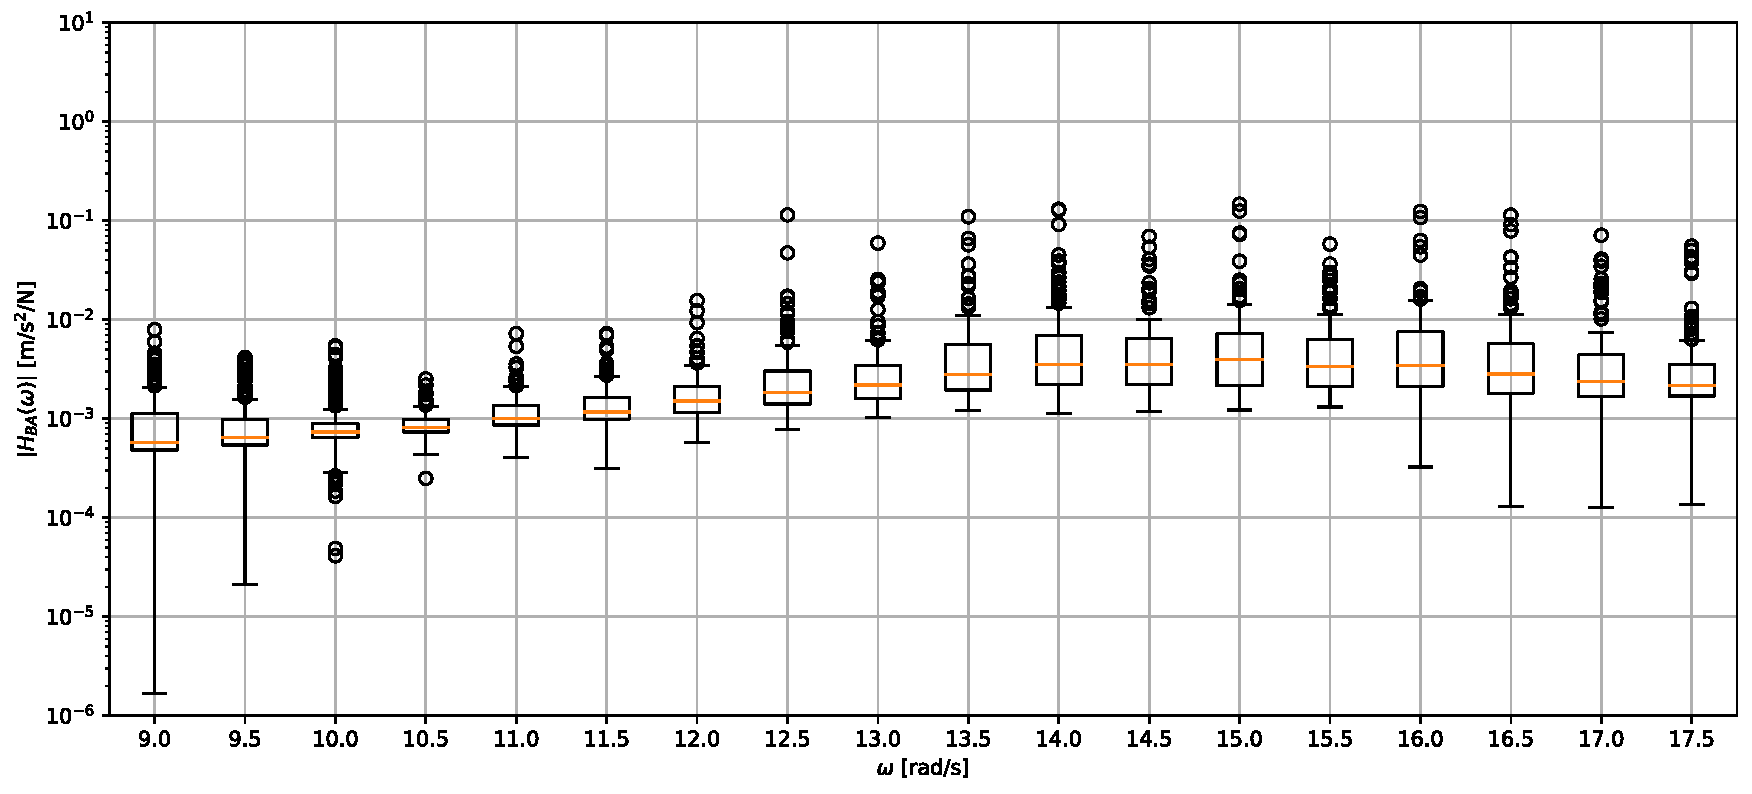
\includegraphics[width=1.0\textwidth]{
        plots/substructuring/plot_8_log.pdf
    }
    \caption{%
        $\left|H_{BA}\right|$ from Direct MCS of The Complete Plate Model with Outliers
    }
    \label{FRF_MC_B_A_log}
\end{figure}
Figure \ref{e_emp CUCB_B_A} shows the median relative empirical errors for the FRFs in each frequency in the above range using three different numbers of internal modes.
The figure exhibits a similar trend with figure \ref{e_emp CUCB_A_A}: as the number of internal modes increases, the relative empirical errors decrease.
\begin{figure}[H]
    \centering
    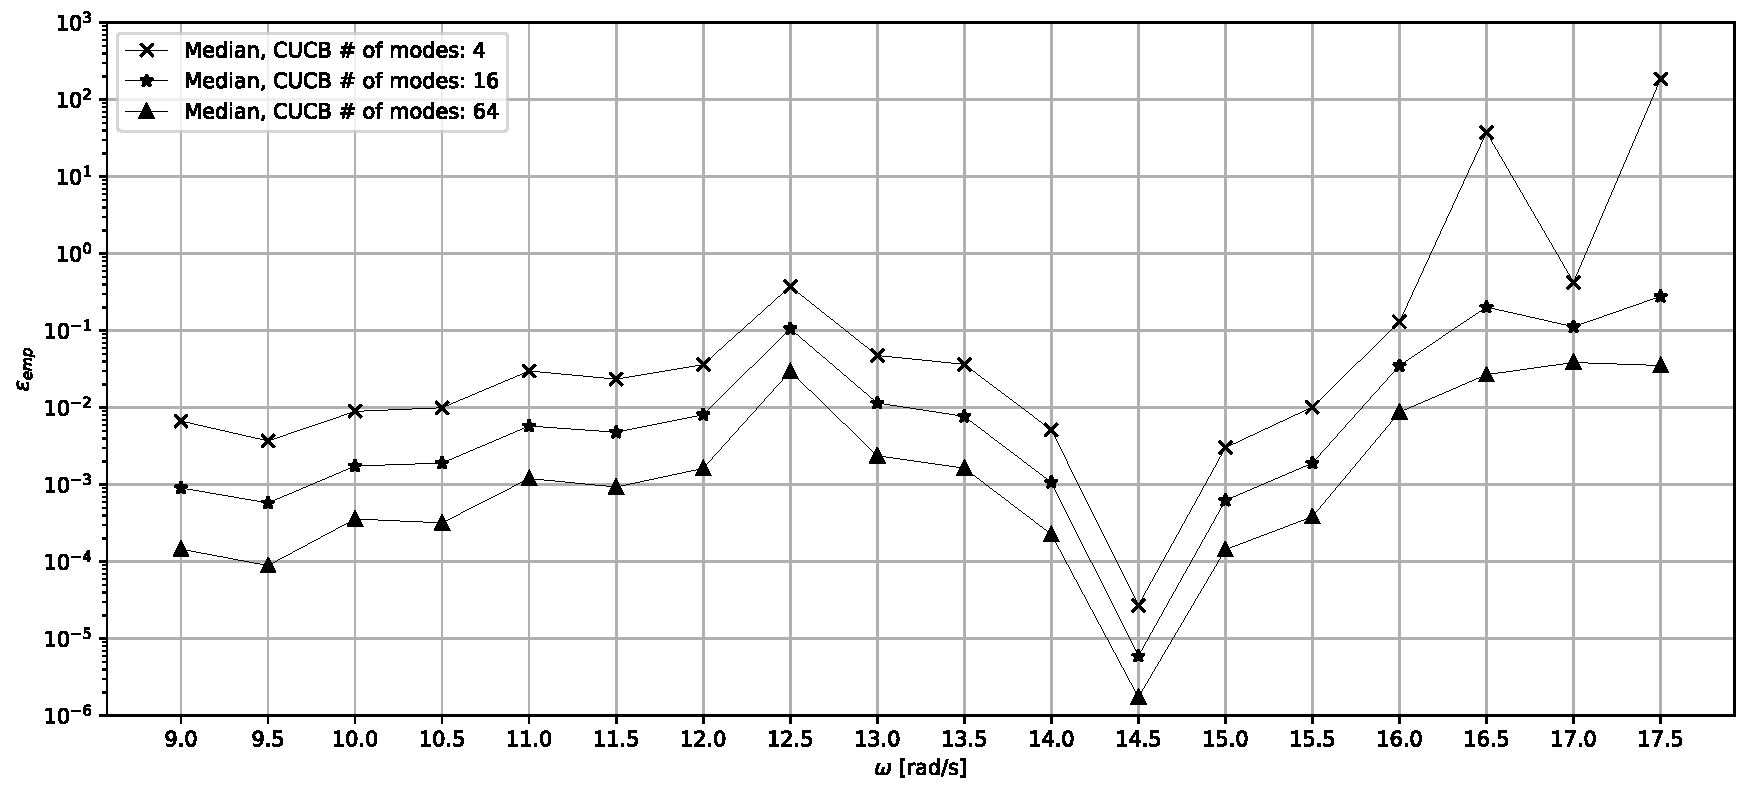
\includegraphics[width=1.0\textwidth]{
        plots/substructuring/plot_9.pdf
    }
    \caption{%
        Relative Empirical Errors of $H_{BA}$ for The CUCB Method
    }
    \label{e_emp CUCB_B_A}
\end{figure}

Figure \ref{e_emp HUCB_B_A} shows the medians and $95\%$ confidence intervals of the relative empirical errors of the FRFs' magnitudes for the crude and hybrid UCB methods.
\begin{figure}[H]
    \centering
    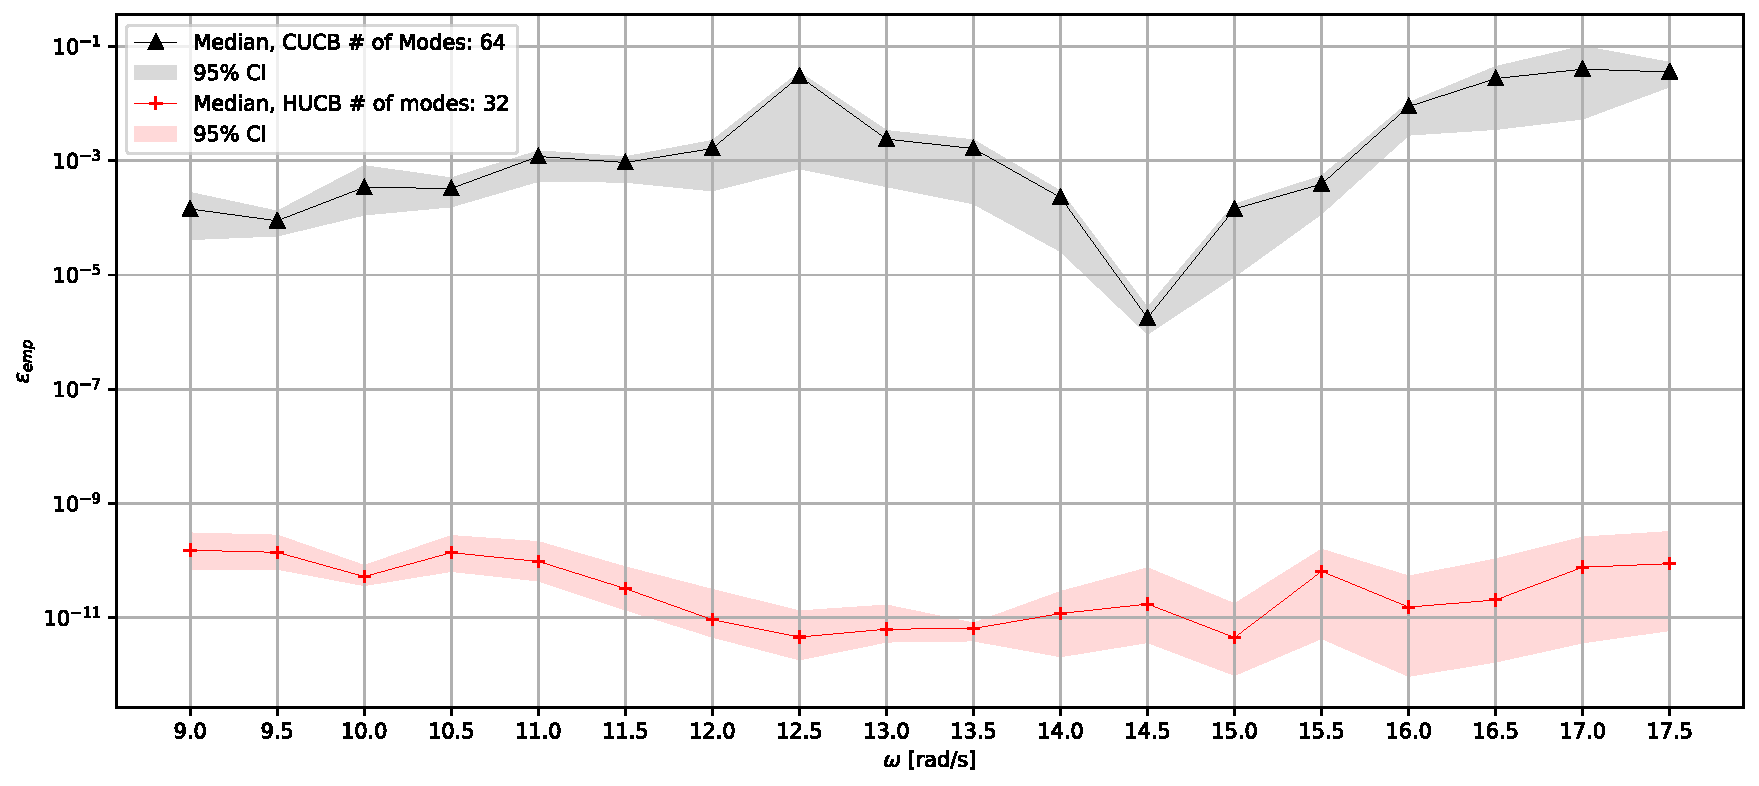
\includegraphics[width=1.0\textwidth]{
        plots/substructuring/plot_10.pdf
    }
    \caption{%
        Relative Empirical Errors of $H_{BA}$ for The CUCB and HUCB Methods
    }
    \label{e_emp HUCB_B_A}
\end{figure}
Comparing figure \ref{e_emp HUCB_A_A} with figure \ref{e_emp HUCB_B_A}, the benefit of the HUCB method over the CUCB method is more pronounced when the force and the response are at two different points or two different components.

Figure \ref{e_mean CUCB_B_A} shows the median relative mean errors of the FRFs' magnitudes for the CUCB method using three different numbers of internal modes.
\begin{figure}[H]
    \centering
    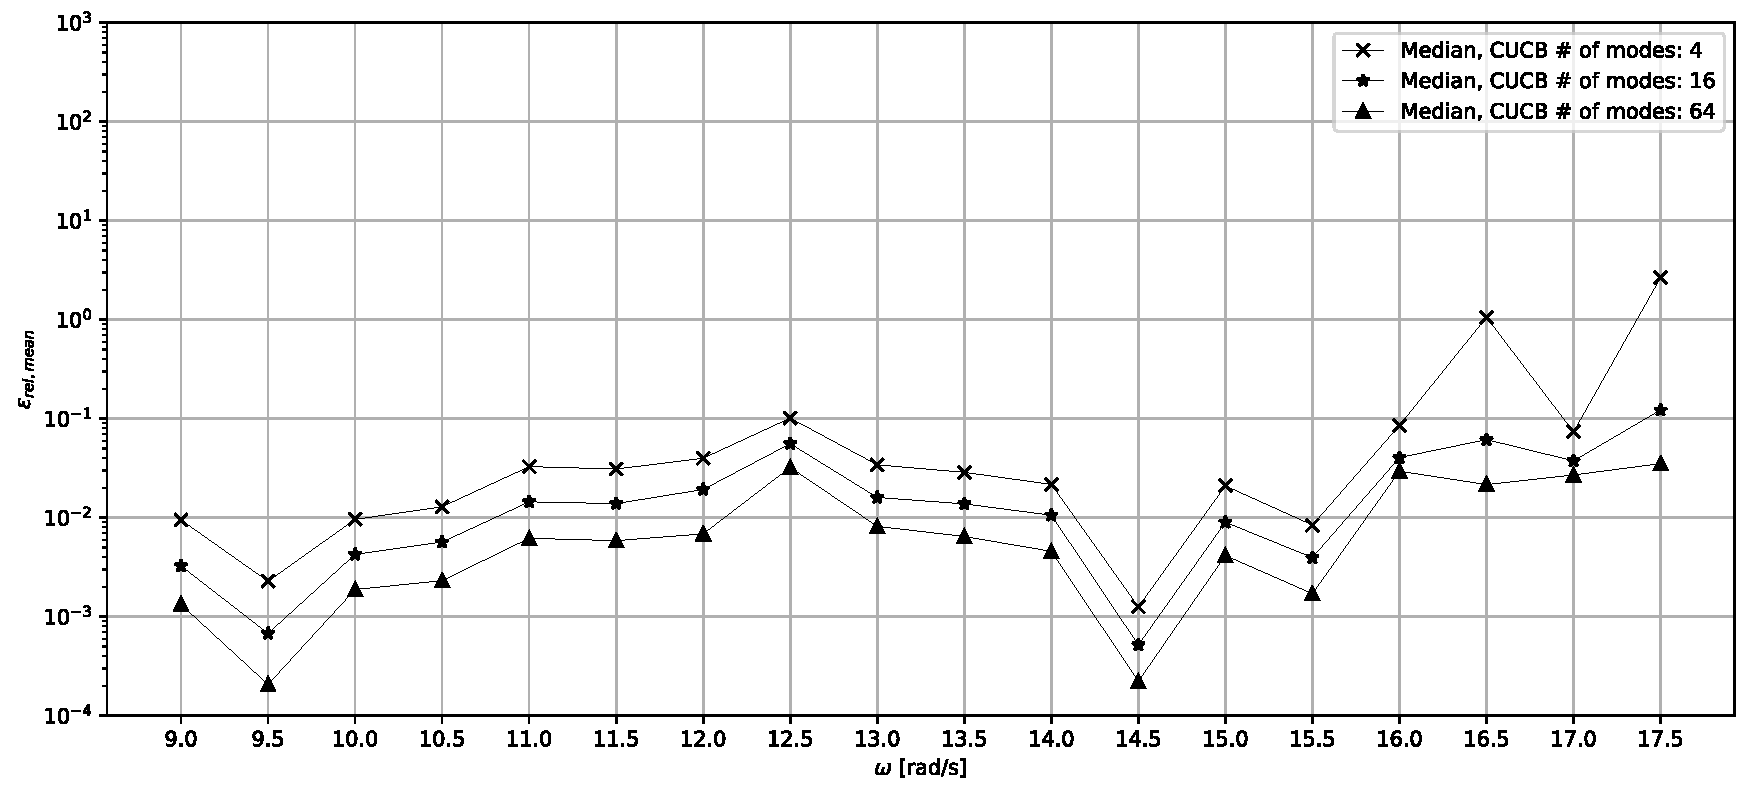
\includegraphics[width=1.0\textwidth]{
        plots/substructuring/plot_11.pdf
    }
    \caption{%
        Relative Mean Errors of $\left|H_{BA}\right|$ for The CUCB Method
    }
    \label{e_mean CUCB_B_A}
\end{figure}
Figure \ref{e_var CUCB_B_A} shows the median relative variance errors of the FRFs' magnitudes for the CUCB method using three different numbers of internal modes.
\begin{figure}[H]
    \centering
    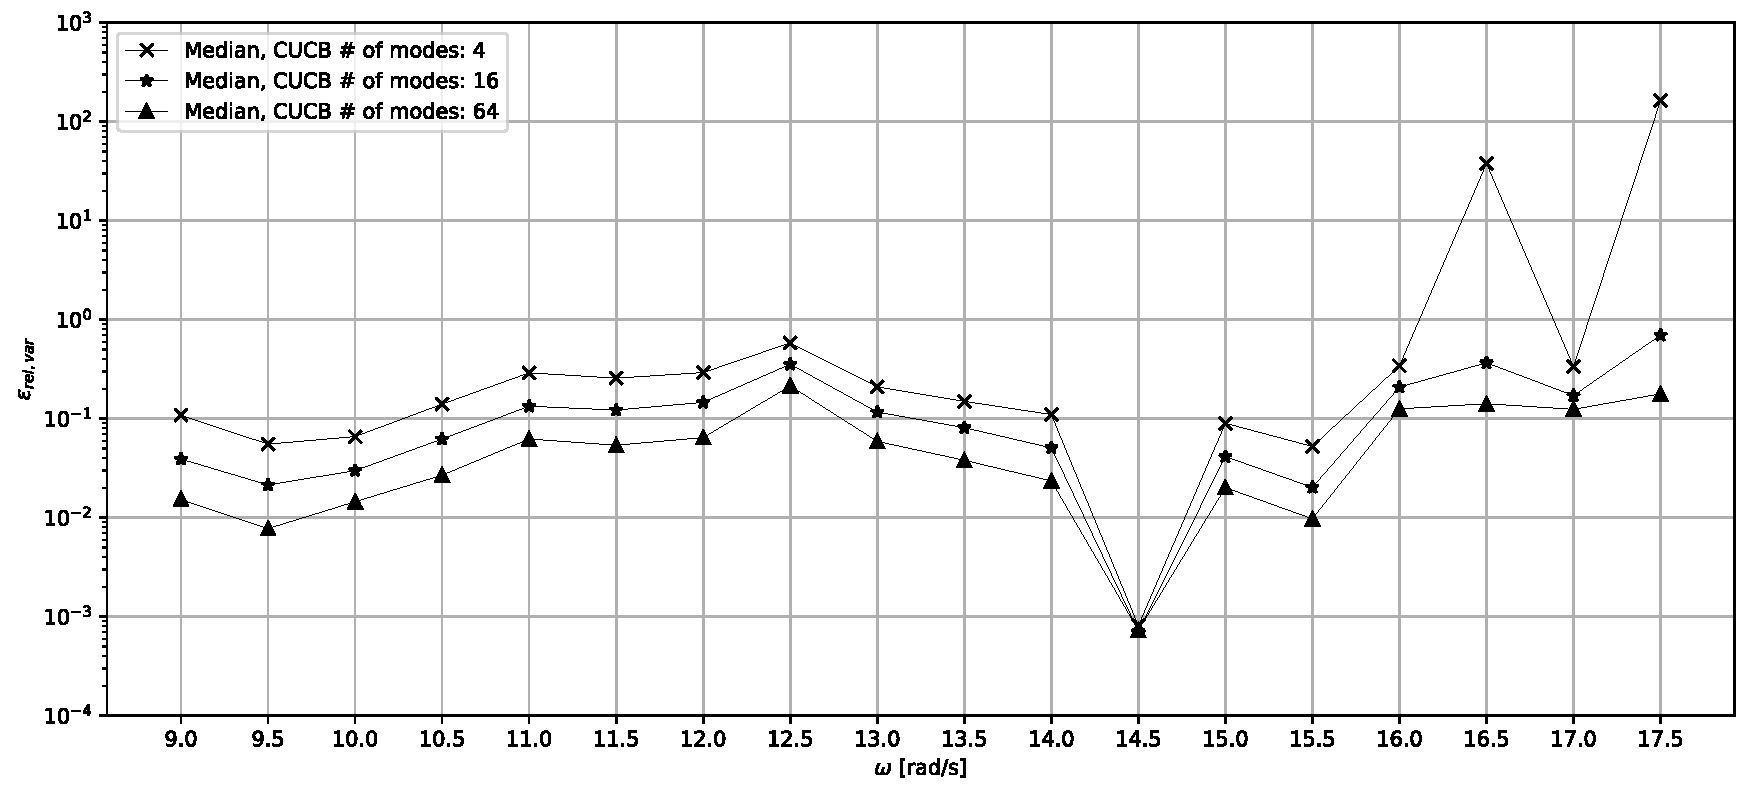
\includegraphics[width=1.0\textwidth]{
        plots/substructuring/plot_12.pdf
    }
    \caption{%
        Relative Variance Errors of $H_{BA}$ for The CUCB Method
    }
    \label{e_var CUCB_B_A}
\end{figure}
The two figures above exhibit similar trends with figure \ref{e_emp CUCB_B_A}: the relative mean errors decrease as the number of internal modes increases.
Overall, the relative mean errors are lower than the relative variance errors.

Figure \ref{e_mean HUCB_B_A} shows the medians and $95\%$ confidence intervals of the relative mean errors for the crude and hybrid UCB methods.
\begin{figure}[H]
    \centering
    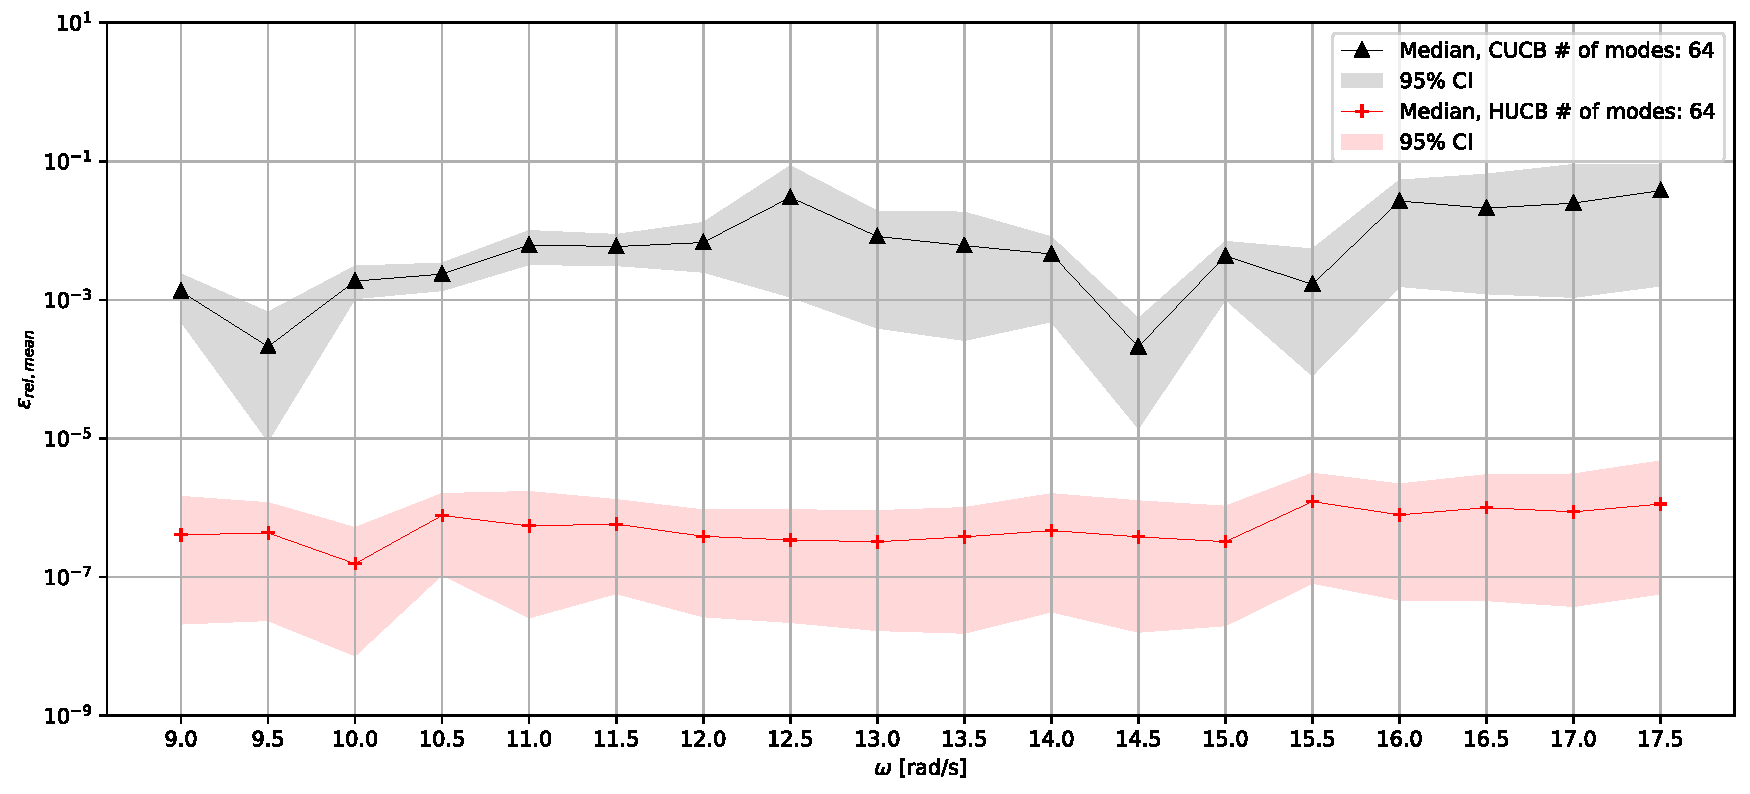
\includegraphics[width=1.0\textwidth]{
        plots/substructuring/plot_13.pdf
    }
    \caption{%
        Relative Mean Errors of $\left|H_{BA}\right|$ for The CUCB and HUCB Methods
    }
    \label{e_mean HUCB_B_A}
\end{figure}
Figure \ref{e_var HUCB_B_A} shows the medians and $95\%$ confidence intervals of the relative variance errors for the crude and hybrid UCB methods.
\begin{figure}[H]
    \centering
    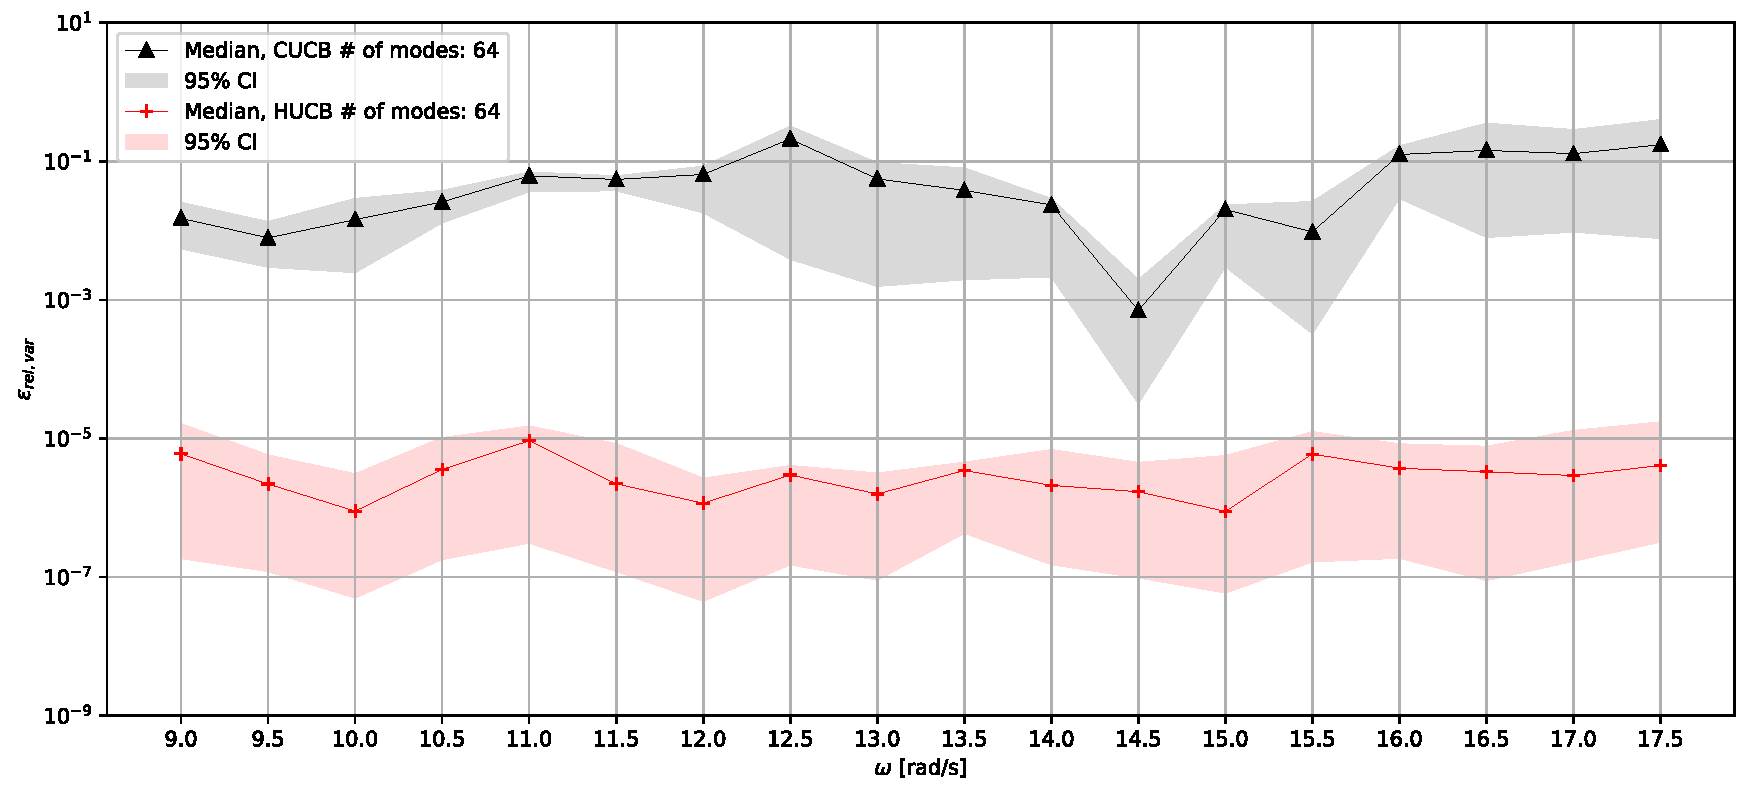
\includegraphics[width=1.0\textwidth]{
        plots/substructuring/plot_14.pdf
    }
    \caption{%
        Relative Variance Errors of $H_{BA}$ for The CUCB and HUCB Methods
    }
    \label{e_var HUCB_B_A}
\end{figure}
The two figures above show that both the relative mean errors and relative variance errors are lower when using the hybrid UCB method by several orders of magnitude.
% -----------------------------------------------------------------------------
% Master thesis in the study program computational mechanics
%
% B.Sc. Rezha Adrian Tanuharja - 03751261
% M.Sc. Felix Schneider (supervisor)
%
% chapters/conclussion.tex
% Last edited 03 November 2023
% -----------------------------------------------------------------------------

\chapter{Summary and Conclusion}
\label{ch: conclusion}

This study has developed a novel framework for uncertainty quantification of large and complex structures by combining the well-established CB method with the recently developed surrogate model, the NI-RPCE model.

The first part of the proposed framework consists of the hybrid UCB method: a modified CB method for models with varying input parameters.
The hybrid UCB method avoids computing the components' internal modes for each realization of input parameters.
The transformation of the structure's equation of motion uses invariant reference internal modes instead.
Consequently, one only needs to solve a generalized eigenproblem for each component, thus reducing the computational cost.

The second part of the proposed framework consists of the sparse NI-RPCE model.
A newly developed procedure selectively removes bases from the model, thus leading to a sparse model.
The sparse RPCE model yields smaller errors compared to the original RPCE model when training data sizes are small.
Consequently, a lower number of evaluations of the structures' dynamic response is necessary, thus further reducing the overall computational cost.

The proposed framework combines the hybrid UCB method with the sparse NI-RPCE models.
It uses the former to generate training data at a lower computational cost, trains the latter using the data, and uses the sparse NI-RPCE models to estimate the structure's dynamic responses.
Consequently, the framework offers two advantages: lower computational cost to generate each training data and reduce the required number of training data.
This study has demonstrated the framework using a case study: a plate clamped at both of its ends, in which the performance of the new framework is satisfactory.

\backmatter

\begin{spacing}{1.0}
  \inputencoding{latin2}
   \bibliography{decorators/literature}
  \inputencoding{utf8}
\end{spacing}

\end{document}